\documentclass[crop=false,class=book]{standalone}
%---------------PREAMBLE------------%
%---------------------------Packages----------------------------%
\usepackage{geometry}
\geometry{b5paper, margin=1.0in}
\usepackage[T1]{fontenc}
\usepackage{graphicx, float}            % Graphics/Images.
\usepackage{natbib}                     % For bibliographies.
\bibliographystyle{agsm}                % Bibliography style.
\usepackage[french, english]{babel}     % Language typesetting.
\usepackage[dvipsnames]{xcolor}         % Color names.
\usepackage{listings, lstlinebgrd}      % Verbatim-Like Tools.
\usepackage{mathtools, esint, mathrsfs} % amsmath and integrals.
\usepackage{amsthm, amsfonts}           % Fonts and theorems.
\usepackage{tabularx}
\usepackage{tcolorbox}                  % Frames around theorems.
\usepackage{upgreek}                    % Non-Italic Greek.
\usepackage{paracol}                    % Two-column styling.
\usepackage{wrapfig}                    % Wrap text around figure.
\usepackage{fmtcount, etoolbox}         % For the \book{} command.
\usepackage[newparttoc]{titlesec}       % Formatting chapter, etc.
\usepackage{titletoc}                   % Allows \book in toc.
\usepackage[nottoc]{tocbibind}          % Bibliography in toc.
\usepackage[titles]{tocloft}            % ToC formatting.
\usepackage{multicol, enumitem}         % Multi-column/enumerate.
\usepackage{import}                     % Import external files.
\usepackage{pgfplots, tikz}             % Drawing/graphing tools.
\usetikzlibrary{
    calc,                   % Calculating right angles and more.
    angles,                 % Drawing angles within triangles.
    arrows.meta,            % Latex and Stealth arrows.
    quotes,                 % Adding labels to angles.
    positioning,            % Relative positioning of nodes.
    decorations.markings,   % Adding arrows in the middle of a line.
    patterns,
    arrows,
    shapes,
    shapes.geometric,
    cd,
    hobby,
    babel
}                                       % Libraries for tikz.
\pgfplotsset{compat=1.9}                % Version of pgfplots.
\usepackage[font=scriptsize,
            labelformat=simple,
            labelsep=colon]{subcaption} % Subfigure captions.
\usepackage[font={scriptsize},
            hypcap=true,
            labelsep=colon]{caption}    % Figure captions.
\usepackage{hyperref}                   % Allows for hyperlinks.
\hypersetup{
    colorlinks=true,
    linkcolor=blue,
    filecolor=magenta,
    urlcolor=Cerulean,
    citecolor=SkyBlue
}                           % Colors for hyperref.
\usepackage[toc,acronym,nogroupskip]{glossaries} % Glossaries and acronyms.
\usepackage[subpreambles=false]{standalone}      % Complileable sub files.

% Various font stuff from kiwi.
% Use this for Times text and Computer Modern math
%\usepackage{times}

% Quite nice
%\usepackage[charter, greekfamily=, greekuppercase=italicized]{mathdesign}
%\usepackage[utopia, greekuppercase=italicized]{mathdesign}    % Math is narrower

% Use this for Times text and math
%\usepackage{newtxtext}
%\usepackage[libertine,cmintegrals]{newtxmath}
%\usepackage{fix-cm}

%\usepackage{txfontsb}
% or
%\usepackage{mathptmx}

%\usepackage[scaled=0.92]{helvet}
%\renewcommand{\rmdefault}{ptm}

%\usepackage{mathpazo}    % add possibly `sc` and `osf` options
%\usepackage{eulervm}

%\usepackage{fourier}
%\renewcommand{\rmdefault}{ptm}
%\usepackage{mathptm}

%\usepackage{fontspec}
%\setmainfont{lmodern}

%\usepackage[varg]{txfonts}
%\usepackage{fouriernc}
%\usepackage{mathpazo}

%\usepackage{bookman}
%\usepackage[scaled]{uarial}
%\usepackage[scaled]{helvet}
%\renewcommand*\familydefault{\sfdefault}
%\usepackage[math]{anttor}

%\newcommand\fgeorgia{\fontfamily{jvn}\selectfont}
%\newcommand\ftimes{\fontfamily{ptm}\selectfont}
%\newcommand\fhelvetica{\fontfamily{phv}\selectfont}
%\newcommand\fcourier{\fontfamily{pcr}\selectfont}
%\newcommand\fbookman{\fontfamily{pbk}\selectfont}
%\newcommand\fnewcentury{\fontfamily{pnc}\selectfont}
%\newcommand\fpalatino{\fontfamily{ppl}\selectfont}
%\newcommand\favantgarde{\fontfamily{pag}\selectfont}
%\newcommand\fnormal{\normalfont}
%\newcommand\fsize[1]{\ifnum#1>0\fontsize{#1}{#1}\selectfont\else\normalsize\fi}
%------------------------Theorem Styles-------------------------%
% Define theorem style for default spacing and normal font.
\newtheoremstyle{normal}
    {\topsep}               % Amount of space above the theorem.
    {\topsep}               % Amount of space below the theorem.
    {}                      % Font used for body of theorem.
    {}                      % Measure of space to indent.
    {\bfseries}             % Font of the header of the theorem.
    {}                      % Punctuation between head and body.
    {.5em}                  % Space after theorem head.
    {}

% Define theorem style for default spacing with italicized font.
\newtheoremstyle{normalit}{\topsep}{\topsep}
                {\itshape}{}{\bfseries}{}{.5em}{}

% Italic header environment.
\newtheoremstyle{thmit}{\topsep}{\topsep}{}{}{\itshape}{}{0.5em}{}

% Define italicized environments.
\theoremstyle{normalit}
\newtheorem{theorem}{Theorem}[section]
\newtheorem{lemma}{Lemma}[section]
\newtheorem{corollary}{Corollary}[section]
\newtheorem{proposition}{Proposition}[section]
\newtheorem*{theorem*}{Theorem}

% Define environments with italic headers.
\theoremstyle{thmit}
\newtheorem*{solution}{Solution}
\newtheorem*{fsolution}{Solution}

% Define default environments.
\theoremstyle{normal}
\newtheorem{example}{Example}[section]
\newtheorem{definition}{Definition}[section]
\newtheorem{problem}{Problem}[section]
\newtheorem{question}{Question}[section]
\newtheorem{remark}{Remark}[section]
\newtheorem{properties}{Properties}[section]
\newtheorem{notation}{Notation}[section]
\newtheorem{axiom}{Axiom}[section]
\newtheorem*{properties*}{Properties}
\newtheorem*{remark*}{Remark}
\newtheorem*{definition*}{Definition}
\theoremstyle{plain}

% Define framed environment.
\tcbuselibrary{most}
\newtcbtheorem[use counter*=theorem]{ftheorem}{Theorem}%
    {colback=green!5,colframe=green!35!black,
     fonttitle=\bfseries\upshape}{th}

\newtcbtheorem[use counter*=example]{fdefinition}{Definition}%
    {fonttitle=\bfseries\upshape,
     colback=blue!5!white,colframe=blue!75!black}{def}

\newtcbtheorem[use counter*=example]{fexample}{Example}%
    {fonttitle=\bfseries\upshape,
     colback=red!5!white,colframe=red!75!black}{ex}

\newtcbtheorem[use counter*=notation]{fnotation}{Notation}%
    {fonttitle=\bfseries\upshape,
     colback=SeaGreen!5!white,colframe=SeaGreen!75!black}{ex}

\newtcbtheorem[use counter*=corollary]{fcorollary}{Corollary}%
    {fonttitle=\bfseries\upshape,
     colback=Orchid!5!white,colframe=Orchid!75!black}{ex}

\newenvironment{bproof}{\textit{Proof.}}{\hfill$\square$}
\tcolorboxenvironment{bproof}{blanker,breakable,left=5mm,
                             before skip=10pt,after skip=10pt,
                             borderline west={1mm}{0pt}{red}}
\tcolorboxenvironment{fsolution}
    {enhanced jigsaw,colframe=cyan,interior hidden,breakable}

%--------------------Declared Math Operators--------------------%
\DeclareMathOperator{\Refl}{Refl}           % Reflection operator.
\DeclareMathOperator{\Span}{Span}           % Span of a set of vectors.
\DeclareMathOperator{\Card}{Card}           % Cardinality of set.
\DeclareMathOperator{\Ord}{Ord}             % Ordinal of ordered set.
\DeclareMathOperator{\Tr}{Tr}               % Trace of matrix.
\DeclareMathOperator{\adjoint}{adj}         % Adjoint of matrix.
\DeclareMathOperator{\rk}{rk}               % Rank of operator.
\DeclareMathOperator{\nul}{nul}             % Null space of operator.
\DeclareMathOperator{\sgn}{sgn}             % Sign of a number.
\DeclareMathOperator{\multideg}{mutlideg}   % Multi-Degree (Graphs).
\DeclareMathOperator{\GCD}{GCD}             % Greatest common denominator.
\DeclareMathOperator{\LM}{LM}               % Leading monomial
\DeclareMathOperator{\LC}{LC}               % Leading coefficient.
\DeclareMathOperator{\LT}{LT}               % Leading term.
\DeclareMathOperator{\LCM}{LCM}             % Least common multiple.
\DeclareMathOperator{\Mon}{Mon}             % Monomial.
\DeclareMathOperator{\Spec}{Spec}           % Spectrum.
\DeclareMathOperator{\proj}{proj}           % Projection.
\DeclareMathOperator{\comp}{comp}           % Component.
\DeclareMathOperator{\sinc}{sinc}           % Sinc function.
\DeclareMathOperator{\Ima}{Im}              % Image of operator.
\DeclareMathOperator{\Prin}{Prin}           % Principal value.
\DeclareMathOperator{\Mod}{mod}             % Modulus.
%------------------------New Commands---------------------------%
\DeclarePairedDelimiter\norm{\lVert}{\rVert}
\DeclarePairedDelimiter\ceil{\lceil}{\rceil}
\DeclarePairedDelimiter\floor{\lfloor}{\rfloor}
\newcommand*\diff{\mathop{}\!\mathrm{d}}
\newcommand*\Diff[1]{\mathop{}\!\mathrm{d^#1}}
\renewcommand{\mod}{\ \Mod}
\renewcommand*{\glstextformat}[1]{\textcolor{RoyalBlue}{#1}}
\renewcommand{\glsnamefont}[1]{\textbf{#1}}
\renewcommand\labelitemii{$\circ$}
\renewcommand\thesubfigure{\arabic{chapter}.\arabic{figure}}
\renewcommand\thesubfigure{%
    \arabic{chapter}.\arabic{figure}.\arabic{subfigure}}
\addto\captionsenglish{\renewcommand{\figurename}{Fig.}}
%------------------------Book Command---------------------------%
\makeatletter
\renewcommand\@pnumwidth{1cm}
\newcounter{book}
\renewcommand\thebook{\@Roman\c@book}
\newcommand\book{%
    \if@openright
        \cleardoublepage
    \else
        \clearpage
    \fi
    \thispagestyle{plain}%
    \if@twocolumn
        \onecolumn
        \@tempswatrue
    \else
        \@tempswafalse
    \fi
    \null\vfil
    \secdef\@book\@sbook
}
\def\@book[#1]#2{%
    \ifnum \c@secnumdepth >-3\relax
        \refstepcounter{book}%
        \addcontentsline{toc}{book}{
            \bookname\ \thebook:\hspace{1em}#1
        }
    \else
        \addcontentsline{toc}{book}{#1}%
    \fi
    \markboth{}{}%
    {\centering
     \interlinepenalty \@M
     \normalfont
     \ifnum \c@secnumdepth >-2\relax
       \huge\bfseries \bookname\nobreakspace\thebook
       \par
       \vskip 20\p@
     \fi
     \Huge \bfseries #2\par}%
    \@endbook}
\def\@sbook#1{%
    {\centering
     \interlinepenalty \@M
     \normalfont
     \Huge \bfseries #1\par}%
    \@endbook}
\def\@endbook{
    \vfil\newpage
        \if@twoside
            \if@openright
                \null
                \thispagestyle{empty}%
                \newpage
            \fi
        \fi
        \if@tempswa
            \twocolumn
        \fi
}
\newcommand*\l@book[2]{%
    \ifnum \c@tocdepth >-2\relax
        \addpenalty{-\@highpenalty}%
        \addvspace{2.25em \@plus\p@}%
        \setlength\@tempdima{3em}%
        \begingroup
            \parindent \z@ \rightskip \@pnumwidth
            \parfillskip -\@pnumwidth
            {
                \leavevmode
                \Large \bfseries #1\hfil \hb@xt@\@pnumwidth{
                    \hss #2
                }
            }
            \par
            \nobreak
            \global\@nobreaktrue
            \everypar{\global\@nobreakfalse\everypar{}}%
        \endgroup
    \fi}
\newcommand\bookname{Book}
\renewcommand{\thebook}{\texorpdfstring{\Numberstring{book}}{book}}
\providecommand*{\toclevel@book}{-2}
\makeatother
\titlecontents{chapter}[0pt]
    {\bfseries}
    {\chaptername\ \thecontentslabel:\quad}
    {}
    {\hfill\contentspage}
\titleformat{\part}[display]
    {\Large\bfseries}
    {\partname\nobreakspace\thepart}
    {0mm}
    {\Huge\bfseries}
    \titlecontents{part}[0pt]
    {\large\bfseries}
    {\partname\ \thecontentslabel: \quad}
    {}
    {\hfill\contentspage}
\newcommand{\MarkRightAngle}[4][.3cm]
    {\coordinate (tempa) at ($(#3)!#1!(#2)$);
     \coordinate (tempb) at ($(#3)!#1!(#4)$);
     \coordinate (tempc) at ($(tempa)!0.5!(tempb)$);%midpoint
     \draw (tempa) -- ($(#3)!2!(tempc)$) -- (tempb);}
%--------------------------LENGTHS------------------------------%
% Spacings for the Table of Contents.
\addtolength{\cftsecnumwidth}{1ex}
\addtolength{\cftsubsecindent}{1ex}
\addtolength{\cftsubsecnumwidth}{1ex}
\addtolength{\cftfignumwidth}{1ex}
\addtolength{\cfttabnumwidth}{1ex}

% Spacing for multi-column and enumerate environments.
\setlength{\multicolsep}{6pt}
\setlist[enumerate]{itemsep=0pt,topsep=3pt}

% Indent and paragraph spacing.
\setlength{\parindent}{0em}
\setlength{\parskip}{0em}
%---------------GLOSSARY------------%
\makeglossaries
\loadglsentries{../../glossary}
\loadglsentries{../../acronym}
%--------------Title Page-----------%
\begin{document}
\chapter{Miscellaneous Materials}
\section{Naif Toolkit}
\subsection{Tutorials}
\subsubsection{Tutorial 1: Introduction}
The objective of this tutorial is to provide an overview of the SPICE system. Information on Fortran, C, IDL, and MATLAB will also be included throughout. The topics of Kernel production and Archiving SPICE data is not addressed in much detail. Math skills, an innate sense of spatial orientation, and familiarity with your computer's OS, a code editor, and a compiler will help. 
\subsubsection{Tutorial 2: Motivation}
Scientists would like to use common tools and methods throughout a project's lifecycle and understand the calculations and transformations used to produce observation geometry data. They'd also like to produce custom geometry calculations themselves. Prior to SPICE was SEDR (Supplemental Experiment Data Record). This was built and operated at JPL. Late or post-launch updates were difficult and expensive to accommodate. Thus, scientists can't get better ancillary data if/when better inputs (Spacecraft trajectory/orientation) are determined. Then came SPICE. SPICE has greater flexibility in deciding what observation geometry parameters are computed, at what times or what frequency for what time span these parameters are computed, and when to re-do parameter computations using new inputs. The downside is there are non-trivial programming requirements needed to read SPICE data and compute whatever is needed. 
\subsubsection{Tutorial 3: Overview}
The original focus of SPICE was on ancillary data needed by planetary scientists for initial science data analysis, science archive preparation, and post-mission data analysis. SPICE now covers the full mission lifecycle and archive uses. It is also used in Heliophysics, Earth Science, observations from terrestrial observatories, and national defense. Ancillary data includes reference frames, positions, orientations, sizes/shapes, pointing, and time conversions. These help determine where the spacecraft is located, and what was the location, size, shape, and orientation of the target being observed. Ancillary data comes from the spacecraft, from the mission control center, from spacecraft and instrument builders, and from science organizations. SPICE is used to organize and package these data in a collection of stable file types called 'Kernels.' Knowing observation geometry and events is an important element of space mission design, selection of observation opportunities, analysis of returned science data from the instruments, mission engineering activities, and preparation o science data archives. SPICE is comprised of the following components:
\begin{enumerate}
\begin{multicols}{3}
    \item Ancillary data files
    \item Software
    \item Documentation
    \item Tutorials
    \item Programming Lessons
    \item Training Classes
    \item User consultation
\end{multicols}
\end{enumerate}
SPICE stands for Spacecraft Planet Instrument C-matrix (Camera matrix) Events. SPICE Data consists of the folowing:
\begin{enumerate}
    \item SPK files deal with the spacecraft and the planets involved. This includes the ephemerides.
    \item PcK files detail the target bodies size, shape, and orientation.
    \item IK files have the instrument field-of-view size, shape, and orientation.
    \item CK files contain the orientation of the space vehicle or any articulating structure on it.
    \item EK (ESP, ESQ, ENB) files contain event information (Science plan, sequence, experiment's notebook).
    \item FK files have reference frame specifications.
    \item LSK is leap seconds tabulation.
    \item SCLK has spacecraft clock coefficients.
    \item DSK has digital shape models.
\end{enumerate}
\begin{figure}[H]
	\centering
	\begin{subfigure}[b]{0.49\textwidth}
	    \includegraphics[width=\textwidth]{NAIF_1}
    \end{subfigure}
    \begin{subfigure}[b]{0.49\textwidth}
        \includegraphics[width=\textwidth]{NAIF_2}
    \end{subfigure}
	\begin{subfigure}[b]{0.49\textwidth}
	    \includegraphics[width=\textwidth]{NAIF_3}
    \end{subfigure}
    \begin{subfigure}[b]{0.49\textwidth}
        \includegraphics[width=\textwidth]{NAIF_4}
    \end{subfigure}
        \caption{Figures from NAIF}
        \label{fig:first_naif_image_more_stuff_4}
\end{figure}
The SPK files contain the space vehicle ephemeris, or trajectory. It also contains the ephemerides of the target planet, satellites, comets, and asteroids. More generally it contains the position of something relative to something else. The PcK files have planet, satellite, comet, and asteroid orientations, shapes, and sizes. Other similar constants such as parameters for gravitational models, atmospheric models, or ring models may also be contained in these. IK files have the instrument field-of-view size, shape, and orientation. Additional information such as internal timing may also exist. CK files have the instrument platform attitude (Or spacecraft attitude). More generally, the orientation of something relative to a specified reference frame. EK files have events broke into three components: ESP, science observation plans; ESQ, spacecraft and instrument commands; ENB, experiment notebooks and ground data system logs. FK files contain the frames. These are definitions and specifications of relationships between reference frames. Both fixed and dynamics frames are available. LSK files contain leap seconds tabulation. Used for converting between UTC and TDB (ET). SCLK files contain spacecraft clock coefficients. Used for converting from SCLK to TDB (ET). DSK files have shape models (Digital elevation model and tesselated planet model). SPICE is available in Fortran 77, C, IDL, MATLAB, and Python. It is also available for Linux, Windows, OSX, and Solaris. An example of using SPICE is as follows: The kernels are selected and incorporated into the User's own modules and SPICE Toolkit library modules. The end result may be an evaluation of a planned orbit, instrument pointing plane, observation geometry visualization, and analysis of expected communications link performance. Instrument data, derived observation geometry, and instrument calibration data may then be analyzed by the user and lead to wonderful science results. SPICE can be used for:
\begin{enumerate}
    \item Evaluation of a planned trajectory
    \item Mission engineering analysis
    \item Planning an instrument pointing profile
    \item Observation geometry visualization
    \item science data archiving and analysis
\end{enumerate}
Many observation geometry parameters at selected times may be computed such as positions, velocities, size, shape, and orientation of planets, satellites, comets, asteroids, and spacecraft. The instrument field-of-view location on a planet's surface or atmosphere may also be computed. Times when a certain geometric event or condition occurs may be found such as eclipses, occultations, conjunctions, and oppositions.
\subsubsection{Tutorial 4: Fundamental Concepts}
\begin{definition}
An Epoch is an instant in time specified by some singular event.
\end{definition}
\begin{example}
Passage of a star across one's zenith meridian.
\end{example}
\begin{example}
Eclipse of a spacecraft signal as it passes behind a solid body.
\end{example}
\begin{remark}
Clocks count epochs specified by events such as "Regular," osciallation of a pendulum, quartz crystal, or electromagnetic radiation from a specified source, measured from an agreed upon reference epoch.
\end{remark}
\begin{definition}
Time Systems are agreed upon standards for naming epochs, measuring time, and synchronizing clocks.
\end{definition}
\begin{definition}
International Atomic Time (TAI) is a statistical time scale based on data from $\sim200$ atomic clocks in over $50$ national laboratories. The unit of a second is the duration of 9,192,631,770 periods of the radiation corresponding to the transition between two hyperfine levels of the ground state of the Cesium $133$ atom. TAI is expressed as a count of atomic seconds past the astronomically determined instant of midnight January 1, 1958 00:00:00.
\end{definition}
\begin{definition}
Coordinate Universal Time (UTC) is the civil time in Greenwich, England ($\sim$GMT).
\end{definition}
\begin{equation}
TAI=UTC+10\ \textrm{seconds}+\textrm{number of leap seconds}
\end{equation}
\begin{remark}
This equation is only valid after January 1, 1972.
\end{remark}
\begin{definition}
Astronomical Time (UT1) is an hour representation of the angle between the plane containing the Greenwich Zenith Meridian (The Prime Meridian) and the plane containing the computed mean sun.
\end{definition}
\begin{remark}
UTC noon and UT1 noon should occur simultaneously. The Earth's rotation is not uniform, and eventually UTC noon and UT1 noon become out of sync. When the mismatch is greater than $0.9$ atomic seconds, a leap second is added or removed from the end of a designated UTC day. Normally June 30 or December 31. The variations in the Earth's rotation that cause this are not predictable.
\end{remark}
\begin{definition}
Barycentric Dynamical Time (TDB) is a mathematical idea used in the equations of motion and is used as the independent time variable for many SPICE subroutine interfaces. It is related to Barycentric Coordinated Time (TCB) by an offset and a scale factor. 
\end{definition}
\begin{definition}
Terrestrial Dynamical Time is the ideal time (Proper time) on Earth at sea level. The IAU calls this Terrestrial Time (TT).
\end{definition}
\begin{equation}
TDT=TAI+32.184\ \textrm{seconds}
\end{equation}
\begin{remark}
TDB and TDT have the same reference epoch, but advance at different rates. Variations are small ($\sim 1.6$ ms) and are almost periodic with a period of 1 sidereal year (To first order). Below describes the variations due to relativistic effects:
\begin{equation}
TDB=TDT+0.001657\sin\big(E+0.01671\sin(E)\big)
\end{equation}
\end{remark} 
Spacecraft have onboard clocks to control scheduling of observations, maneuvers, and attitude adjustments and are used to time stamp data. The fundamental unit of time for these is the tick, which is the smallect increment possible for a spacecraft clock. Nominal tick duration is spacecraft clock dependent. SCLK string formats vary for different spacecraft. 
\begin{definition}
A reference frame is an ordered set of three mutually orthogonal, and possibly time dependent, unit direction vectors, coupled with a location called the frame's origin.
\end{definition}
\begin{definition}
The ordered set of axes of a reference frame is called a basis.
\end{definition}
\begin{definition}
A coordinate system is the method of locating points in a given reference frame.
\end{definition}
\begin{example}
Cartersian coordinate systems and Spherical coordinate systems are very common for $\mathbb{R}^3$ (3-dimensions).
\end{example}
\begin{remark}
A reference frame's center is an ephemeris object whose location is coincident with the origin of the frame. The center of the a body is the center of mass of the body. The center of any inertial frame is the solar system barycenter (In SPICE).
\end{remark}
The origin cancels in vector arithmetic, so choice of center is somewhat unimportant. Choice of axes is more important. The center is used in computing light time to centers of non-inertial frames.
\begin{definition}
An inertial reference frame is a reference frame that satisfies the following conditions:
\begin{enumerate}
    \item It is non-rotating with respect to fixed stars.
    \item The origin is non-accelerating.
\end{enumerate}
\end{definition}
\begin{remark}
The velocity of the origin is typically non-zero, and the actual acceleration is negligible.
\end{remark}
\begin{example}
J2000 (Also called ICRF) and B1950 are inertial reference frames.
\end{example}
\begin{definition}
A non-inertial reference frame is a reference frame that is not an inertial reference frame.
\end{definition}
\begin{example}
Body-fixed reference frames, those centered at a body center or topocentric, are non-inertial (Unless the body is the Sun or the galactic center, etc.) The reference frame of an instrument is non-inertial. Dynamic frames (Frames defined by time-dependent vectors) are non-inertial as well.
\end{example}
\begin{definition}[\textbf{J2000 Frame}]
The J2000 frame is defined by the Earth's equator and equinox, determined from observations of planetary motions and other data. 
\begin{enumerate}
    \item The $x-$axis is the line of intersection between Earth's mea equatorial plane and the ecliptic plane on January 1, 2000 12:00:00 TDB, or JD 2451545.0 TDB.
    \item The $z-$axis is the line normal to the mean equatorial plane which contains the Earth's core on January 1, 2000 12:00:00 TDB. It is approximately equal to the Earth's spin axis orientation at that epoch.
    \item The $y-$axis is defined as the line that contains the intersection of the $x$ and $z$ axis and is parallel to $\hat{\mathbf{z}}\times \hat{\mathbf{x}}$, where $\hat{\mathbf{z}}$ and $\hat{\mathbf{x}}$ are unit vectors for the $z$ and $x$ axes, respectively.
\end{enumerate}
\end{definition}
\begin{figure}
    \centering
    \includegraphics[width = \textwidth]{NAIF_5}
    \caption{Example of the J2000 Frame}
    \label{fig:naif_j200_figure}
\end{figure}
Body-fixed frames are tied to a named body and rotate with it. The most common bodies are hard-coded in SPICE "IAU\_Body Name"
\begin{example}
IAU\_MARS, IAU\_SATURN
\end{example}
The rotation state (Orientation at time T) is determined using a SPICE text PCK. 
\begin{remark}
IAU\_EARTH and IAU\_MOON exist, but should NOT be used. See "lunar-earth\_pck-fk" for the best frames for these bodies.
\end{remark}
\begin{definition}
Topocentric frames are reference frames attached to the surface of a body. The $z-$axis lies parallel to the gravity gradient. That is, it points "Up."
\end{definition}
\begin{example}
We can take a point on Earth's surface and say that $\hat{\mathbf{z}}$ points to the zenith, $\hat{\mathbf{x}}$ points North, and thus $\hat{\mathbf{y}}$ points West.
\end{example}
\begin{definition}
Planetocentric coordinate systems are systems such that the origin lies at the center of a given body. $\hat{\mathbf{z}}$ lies parallel to the North Pole.
\end{definition}
\begin{remark}
Dwarf Planets (Pluto, Ceres, Eris, Haumea, Makemake) and other small objects spin in the right hand sense about their "North Pole."
\end{remark}
\begin{definition}
The state of an object is its position and velocity relative to a given object.
\end{definition}
\begin{remark}
In SPICE, these objects are referred to as target and observer. In the SPK subsystem, a state is a six dimensional vector. A state is specified relative to a reference frame.
\end{remark}
\begin{figure}[H]
    \centering
    \begin{subfigure}[b]{0.49\textwidth}
        \centering
        \includegraphics[width=\textwidth]{NAIF_6}
    \end{subfigure}
    \begin{subfigure}[b]{0.49\textwidth}
        \centering
        \includegraphics[width=\textwidth]{NAIF_7}
    \end{subfigure}
    \caption{Aberration Corrections}
    \label{fig:naif_aberration_corrections}
\end{figure}
To perform algebraic operations on states, they must be in the same reference frame. If two reference frames are both right-handed, we may convert between the two via a rotation matrix:
\begin{equation}
P_{B}(t)=R(t)P_{A}(t)
\end{equation}
As both references frames may be time dependent, the rotation matrix may be time dependent. The velocity frame transformation is the time derivative:
\begin{equation}
\frac{dP_{B}(t)}{dt}=\frac{dR(t)}{dt}P_{A}(t)+R(t)\frac{dP_{A}(t)}{dt}
\end{equation}
We have the following transformation between states:
\begin{equation}
\begin{pmatrix}P_{B_{x}}(t)\\P_{B_{y}}(t)\\P_{B_{z}}(t)\\ \frac{dP_{B_{x}}(t)}{dt}\\ \frac{dP_{B_{y}}(t)}{dt}\\ \frac{dP_{B_{z}}(t)}{dt}\end{pmatrix}=
\begin{pmatrix}R_{11}(t)&R_{12}(t)&R_{13}(t)&0&0&0\\R_{21}(t)&R_{22}(t)&R_{23}(t)&0&0&0\\R_{31}(t)&R_{32}(t)&R_{33}(t)&0&0&0\\\frac{dR_{11}(t)}{dt}&\frac{dR_{12}(t)}{dt}&\frac{dtR_{13}}{dt}&R_{11}(t)&R_{12}(t)&R_{13}(t)\\\frac{dR_{21}(t)}{dt}&\frac{dR_{22}(t)}{dt}&\frac{dtR_{23}}{dt}&R_{21}(t)&R_{22}(t)&R_{23}(t)\\
\frac{dR_{31}(t)}{dt}&\frac{dR_{32}(t)}{dt}&\frac{dtR_{33}}{dt}&R_{31}(t)&R_{32}(t)&R_{33}(t)\end{pmatrix}
\begin{pmatrix}P_{A_{x}}(t)\\P_{A_{y}}(t)\\P_{A_{z}}(t)\\ \frac{dP_{A_{x}}(t)}{dt}\\ \frac{dP_{A_{y}}(t)}{dt}\\ \frac{dP_{A_{z}}(t)}{dt}\end{pmatrix} 
\end{equation}
Where $R_{ij}(t)$ is the $i^{th}$ row $j^{th}$ column of the rotation matrix $R(t)$. The SPICELIB routine SXFORM and PXFORM return state transformation and position transformation matrices, respectively. Within the SPICE System, Aberration Corrections are adjustments made to state vectors and time-dependent reference frames to accurately reflect the apparent (As opposed to actual) state and attitude of a target object as seen from a specified observer at a specified time. Actual uncorrected states from an ephemeris are called geometric states. Aberration corrections are need to accurately answer the following:
\begin{enumerate}
    \item Which direction must a remote sensing instrument point to observe a target of interest?
    \item For a given pointing direction and observation time, what target body surface location would be observed by a remote sensing instrument?
    \item Which direction must an antenna be pointed to transmit a signal to a specified target?
\end{enumerate}
\subsubsection{Tutorial 5: Conventions}
\begin{enumerate}
    \item SPICE - The name of this ancillary information system.
    \item NAIF - The name of the team of people at KPL who lead development of the SPICE system.
    \item SPICE Toolkit - The principal collection of software produced by NAIF as part of the SPICE information system.
    \item Toolkit - The Fortran 77 version of the SPICE Toolkit.
    \item Kernel - A SPICE data file.
    \item SPICELIB - The principal user library found within the Fortran versions of the SPICE Toolkit.
    \item CSPICE - The C Toolkit, and the principal user library within C versions of the SPICE Toolkit.
    \item Icy - An IDL interface to CSPICE.
    \item Mice - A MATLAB interface to CSPICE.
    \item Text Kernel - Kernels consisting entirely of ASCII information, each line terminated using the local OS convention.
    \item Binary Kernel - Any kernel type using a binary file format. Binary types are SPK, binary PcK, CK, DBK, and DSK.
    \item Transfer format kernel - A hexadecimal (ASCII) version of a binary kernel.
    \item Command File - An input file containing program directives, and sometimes input data.
    \item Found Flag - Boolean output that informs your program whether or not data were found that match your request.
    \item Database Kernel (DBK) - A kernel that provides a self-contained SQL-like database capability.
    \item Coverage - The period of time for which a time-based kernel contains data.
    \item Deprecated software - Code that has been superseded with a new and presumably better version.
    \item Toolkit Version Naming -``Nxxxx", e.g. N0065 is Version 65.
    \item Satellite - A natural satellite, never a spacecraft.
    \item Run-time - Occurs when you execute a program.
\end{enumerate}
SPICE imposes some restrictions on kernel files names. No white space allowed and a maximum of 255 characters. NAIF suggests names conform to PDF standard: "36.3." Below lists common SPICE Kernel File Name Extensions. All reference frames used within SPICE are right-handed systems. That is, $\hat{\mathbf{x}} = \hat{\mathbf{y}}\times \hat{\mathbf{z}}$. SPICE also uses quaternions in C-kernels. There are different definitions of quaternions based on the order of the quaternion elements, the multiplication formula, and the convention for associating quaternions with rotation matrices. The two commonly used styles are SPICE, which is Hamilton's original formulation, and MSOP, which is used in attitude control and other aerospace applications.
\begin{table}[H]
    \centering
    \resizebox{\textwidth}{!}{
    \begin{tabular}{|ccl|ccl|ccl|}
        \hline
        SPK&&&SCLK&&&PcK&&\\
        \hline
        &.bsp&Binary SPK file.&&.tsc&Text SCLK file.&&.tpc&Text PcK file.\\
        &.xsp&Transfer format SPK file.&&&&&.bpc&Binary PcK file.\\
        &&&&&&&.xpc&Transfer format PcK file.\\
        \hline
        MK&&&IK&&&DSK&&\\
        \hline
        &.tm&Text meta-kernel file.&&.ti&Text IK file.&&.bds&Binary DSK file.\\
        \hline
        FK&&&LSK&&&CK&&\\
        \hline
        &.tf&Text FK file.&&.tls&Text LSK file.&&.bc&Binary CK file.\\
        &&&&&&&.xc&Transfer format CK file.\\
        \hline
        ESP&&&ESQ&&&ENB&&\\
        &.bep&Binary science plan EK file.&&.bes&Binary sequence component EK file.&&.ten&Text experimenter's notebook EK file.\\
        &.xep&Transfer format science plan EK file.&&.xes&Transfer format sequence component EK file.&&&\\
        \hline
        DBK&&&DBK&&&&&\\
        &.bdb&Binary database kernel.&&.xdb&Transfer format database kernel.&&&\\
        \hline
    \end{tabular}}
    \caption{List of Kernel File Types}
    \label{tab:naif_list_of_kernel_file_types}
\end{table}
\begin{remark}
Pluto is a special case. Pluto is treated as a planet when speaking about ephemerides (SPK). Pluto is treated as a dwarf planet when speaking about orientation and rotational state (PCK).
\end{remark}
\subsubsection{Tutorial 6: IDs}
SPICE uses IDs and names to identify physical objects and reference frames. An ID is an integer number and a name is a string. Names are used primarily as input and output arguments in SPICE software interfaces (APIs). User's deal mostly with names. Physical object IDS are used in kernels as data identifies. Physical object names are used in the high-level user APIs as input and/or output arguments. 
\begin{enumerate}
    \item Spacecraft are negative numbers.
    \begin{itemize}
    \begin{multicols}{3}
        \item $-6$ is PIONEER 6
        \item $-64$ is OSIRIS-REX
        \item $-82$ is Cassini
    \end{multicols}
    \end{itemize}
    \item DSN Ground Stations are $399000+\textrm{Station Number}$
    \begin{itemize}
    \begin{multicols}{2}
        \item $399005$ is DSS-05
        \item $399066$ is DSS-66
    \end{multicols}
    \end{itemize}
    \item Non\_DSN stations are $39800+$ an integer between $0$ and $999$: $398990$ is New Norcia
    \item The sun is $10$ and the Solar System Barycenter is $0$.
    \item The planet barycenters are $1-9$
    \begin{itemize}
    \begin{multicols}{3}
        \item[] $1$ - Mercury Barycenter
        \item[] $2$ - Venus Barycenter
        \item[] $3$ - Earth-Moon Barycenter
        \item[] $4$ - Mars Barycenter
        \item[] $8$ - Neptune Barycenter
        \item[] $9$ - Pluto Barycenter
    \end{multicols}
    \end{itemize}
    \item Satellites are the planet barycenter number multiplied by a number between $1$ and $98$.
    \begin{itemize}
    \begin{multicols}{4}
        \item $301$ - The Moon
        \item $401$ - Phobos
        \item $402$ - Deimos
        \item $501$ - Io
    \end{multicols}
    \end{itemize}
    \item Periodic comets are $1000000 +$ sequence number.
    \begin{itemize}
    \begin{multicols}{2}
        \item $1000001$ - Arend
        \item $1000002$ - Agen-Regaux
        \item $100036$ - Halley
        \item $100132$ - Hale-Bopp
    \end{multicols}
    \end{itemize}
    \item Numbered Asteroids are $2000000+$ IAU asteroid number.
    \begin{itemize}
    \begin{multicols}{3}
        \item $2000001$ - Ceres
        \item $2000004$ - Vesta
        \item $2009969$ - Braille
    \end{multicols}
    \end{itemize}
    \item Science instruments are the spacecraft number times $1000$, minus the instrument number.
    \begin{itemize}
    \begin{multicols}{2}
        \item $-82760$ - Cassini MIMI CHEMS
        \item $-82001$ - Cassini SRU-A
    \end{multicols}
    \end{itemize}
\end{enumerate}
\subsubsection{Tutorial 8: Introduction to the Family of SPICE Toolkits}
\begin{figure}[H]
    \centering
    \includegraphics[width=0.9\textwidth]{NAIF_9}
    \caption{Methods of using the toolkit}
    \label{fig:naif_toolkit_and_wrappers}
\end{figure}
``Toolkit," is the Fortran 77 toolkit. Developed first and in use since February 1990. $CSPICE$ is the C-language Toolkit. Designed to duplicate the functionality of the Fortran Toolkit. Icy is the IDL Toolkit. Provides and IDL-callable ``Wrapper," interface for many CSPICE wrapper routines. Mice is the Matlab Toolkit. Mice provides a MATLAB-callable ``Wrapper," interface for many CSPICE wrapper routines. Computations are identical in all languages. 
\subsubsection{Tutorial 9: Icy}
Icy operates as an extension to the IDL language regime and supports more than 300 CSPICE routines. Icy also has some capability not available in CSPICE such as vectorization. The IDL environment includes an intrinsic capability to use external routines. Icy functions as an IDL Dynamically Loadable Module (DLM). A DLM consists of a shared object library (icy.so/.dll) and a DLM text definition file. Using Icy from IDL requires you to register the Icy DLM with IDL to access interface routines. The next question is how does it work. IDL calls the interface routine in the shared object library, linked against CSPICE, which performs its function and returns the result to IDL. A user may occasional encounter an IDL math exception:
\begin{lstlisting}[language=bash,basicstyle=\footnotesize]
% Program caused arithmetic error: Floating underflow
\end{lstlisting}
This warning occurs most often as a consequence of CSPICE math operations. CSPICE assumed numeric underflow as zero, so in all known cases this can be ignored.
\begin{remark}
There is a possible irritant in loading kernels using the cspice\_furnsh function. Kernels are loaded into your IDL session, not into your IDL scripts. This means loaded binary kernels remains accessible (Active). Data from loaded text kernels remain in the kernel pool throughout your IDL session. A consequence is that some kernel data may be available to one of your scripts even though it was not intended to be so. You could get incorrect results. There are two fixes for this:
\begin{enumerate}
    \item Load all needed SPICE kernels for your IDL session at the beginning, paying careful attention to the files loaded and the loading order.
    \item At the end of every IDL script, write cspice\_kclear to remove all kernel data from the kernel pool.
\end{enumerate}
\end{remark}
\subsubsection{Tutorial 12: Introduction to Kernels}
\begin{definition}
A kernel is a file that contains ancillary data. Specifically, low level ancillary data that may be used to determine higher level observation geometry parameters.
\end{definition}
\begin{table}[H]
    \centering
    \resizebox{\textwidth}{!}{
    \begin{tabular}{|cl|cl|cl|}
        \hline
        SPK&&FK&&IK&\\
        &Spacecraft and Planetary Ephemeris&&Reference frame specifications&&Instrument\\
        \hline
        SCLK&&LSK&&CK&\\
        &Spacecraft clock correlation data&&Leapseconds&&Points (C-Matrix)\\
        \hline
        PCK&&DSK&&DBK&\\
        &Planetary constants (orientation, size, shape)&&Digital shape kernel (Tesselated plate, digital elevation models)&&Database mechanism\\
        \hline
        EK&&EK&&EK&\\
        &ESP: Science Plan&&ESQ: Sequence&&ENB: Experimenter's Notebook\\
        \hline
        MK&&MK&&&\\
        &Meta-Kernel&&Mechanism for loading kernel files&&\\
        \hline
    \end{tabular}}
    \caption{Caption}
    \label{tab:my_label}
\end{table}
\begin{definition}
A text kernel is a plain text file of ASCII data, containing assignments of the form $variable=value$
\end{definition}
\subsubsection*{Text Kernel Formatting}
\begin{enumerate}
    \item[]KPL/$<$kernel type$>$
    \begin{enumerate}
        \item[] Tells SPICE what kind of kernel it is.
    \end{enumerate}
    \item[] \textbackslash begindata and \textbackslash begintext
    \begin{enumerate}
        \item[] Markers which set off the beginning of data and meta-data blocks, respectively.
    \end{enumerate}
    \item[] $<$LF$>$ for Unix/Linux/Mac, $<$CR$><$LF$>$ for Windows.
    \begin{enumerate}
        \item[] End of line marker. Must be present on EVERY line in the text kernel.
    \end{enumerate}
    \item[] Max line length, including white space, is 132 characters.
\end{enumerate}
Text kernels may be produced using any text editor. Text kernels must contain human-readable text only. TAB characters are allowed but HIGHLY DISCOURAGED. Text kernels must have each line terminated with the end-of-line indicator (See above). Binary kernels are made using Toolkit utility programs, or by using Toolkit APIs built into your own application program.
\subsubsection{Using Kernels}
To make kernels available to a program they must be loaded. When you load a text kernel, the file is opened, the kernel contents are read into memory, and then the file is closed. When you load a binary kernel, the file is opened, for SPK, CK, and binary PCK, no data are read until a read request is made by Toolkit software. For ESQ files, the schema description is read, checked, and stored in memory at load time, but no data are read until a query/fetch is made. For all practical purposes the binary file remains open unless specifically unloaded by you. Use the FURNSH routine to load all kernels (Text and binary).
\begin{lstlisting}[language=bash,basicstyle=\footnotesize]
IDL> cspice_furnsh, 'name.ext'
\end{lstlisting}
Best practice: Don't hard code filenames, list these in a meta-kernel and load the meta-kernel using FURNSH. Binary kernels, whether or not in native binary format, may be read by any of the toolkits. Text kernels may be read by any of the C, IDL, and MATLAB toolkits.
\subsubsection{Meta-Kernels}
\begin{definition}
A meta-kernel is a file that lists names and locations of a collection of SPICE kernels that are to be used together in a SPICE-based application.
\end{definition}
\begin{remark}
You can simply load the meta-kernel, causing of the kernels listed in it to load.
\end{remark}
Using a metal-kernel makes it easy to manage which SPICE files are loaded into your program. A meta-kernel is implemented using the SPICE text kernel standards.
\begin{example}
Example of a meta-kernel
\begin{lstlisting}[language=bash,basicstyle=\footnotesize]
KPL/MK
 \begindata
  KERNELS_TO_LOAD = (
   '/home/mydir/kernels/lowest_priority.bsp',
   '/home/mydir/kernels/next_priority.bsp',
   '/home/mydir/kernels/highest_priority.bsp',
   '/home/mydir/kernels/leapseconds.tls',
   '/home/mydir/kernels/sclk.tsc',
   '/home/mydir/kernels/c-kernel.bc',
   '/home/mydir/kernels+?,
   '/custom/kernel_data/p_constants.tpc?,
                     )
\end{lstlisting}
Example of a meta-kernel using the PATH\_VALUES and PATH\_SYMBOLS.
\begin{lstlisting}[language=bash,basicstyle=\footnotesize]
KPL/MK
\begindata  
        PATH_VALUES     = ( '/home/mydir/kernels' )
        PATH_SYMBOLS    = ( 'KERNELS'             )
        KERNELS_TO_LOAD = (                       )
            '$KERNELS/lowest+priority.bsp',
            '$KERNELS/next_priority/bsp',
            '$KERNELS/leapseconds.tls',
            '$KERNELS/sclk.tsc',
            '$KERNELS/c-kernel.bc',
            '$KERNELS/custom/kernel_data/p_constants.tpc'
                            )
\end{lstlisting}
\end{example}
The order in which SPICE kernels are loaded at run-time determines their priority when requests for data are made. For binary kernels, data from a higher priority file will be used in the case when two or more files contain data overlapping in time for a given object. For SPKs, CKs, and binary PCKs , the file loaded last takes precedence and has highest priority. Priority doesn't apply to ESQ files. If two or more text kernels assign values to a single keyword using $=$, the data value associated with the last loaded occurrence of the keyword are used. Orientation data from a binary PCK always supersedes orientation data obtained from a text PCK, no matter the order in which the kernels are loaded. The unloading of kernels is essential for Icy and Mice scripts. Because of the way IDL and MATLAB interact with external shared object libraries, any kernels loaded during an IDL or MATLAB session will stay loaded until the end of the session unless they are specifically unloaded. The routines KCLEAR and UNLOAD may be used to unload kernels containing data you wish to be no longer available in your program. KCLEAR unloads all kernels and clears the kernel pool. UNLOAD unloads specified kernels.
\begin{figure}
    \centering
    \includegraphics[width=0.6\textwidth]{NAIF_13}
    \caption{Data structure hierarchy}
    \label{fig:naif_data_structure_hierarchy}
\end{figure}
\subsubsection{Tutorial 13: Comments in SPICE Kernels}
\begin{definition}
Kernel comments, also called meta-data, are information that describe the context of kernel data.
\end{definition}
Comments are provided inside kernels as plain text. Binary kernels have a reserved comment area to hold comments. Text kernels have comments interleaved with the data. Comments may be inserted between blocks of data as follows:
\begin{lstlisting}[language=bash,basicstyle=\footnotesize]
\begintext
	Some Comments
\begindata
	Some data
\end{lstlisting}
To view comments in binary kernels, use either $commnt$ or $spacit$ utility program. To view text kernels, use any text file utility such as more, cat, vi, emacs, Notepad, TextEdit, BBEdit, Word, etc.
\begin{example}
\begin{lstlisting}[language=bash,basicstyle=\footnotesize]
;An example for a binary kernel.
IDL> commnt -r de421.bsp | more
;An example for a text kernel.
IDL> more naif0008.tls
\end{lstlisting}
\end{example}
\subsubsection{Tutorial 14: Using Module Headers}
NAIF uses module headers to provide detailed information describing how to use the module. In FORTRAN, C, and MATLAB, the headers are comment blocks in the source code. For IDL, the headers are independent files. All distributions include plain text and HTML versions. (HTML version is hyperlinked with other NAIF documentation). 
\subsubsection{Tutorial 15: Time Conversions and Time Formats}
Time inputs to and outputs from a user's programs are usually strings representing epochs in the following time systems:
\begin{enumerate}
    \item Ephemeris Time (ET)
    \item Coordinated Universal Time (UTC)
    \item Spacecraft Clock (SCLK)
\end{enumerate}
Time stamps in kernel files, time inputs to SPICE routines, and time outputs from SPICE routines are double precision numbers representing epochs in the following time systems:
\begin{enumerate}
    \item Numeric Ephemeris Time (TDB), expressed as ephemeris seconds past J2000.
    \item Encoded Spacecraft Clock, expressed as clock ticks since the clock start.
\end{enumerate}
SPICE provides routines to convert between these string and numeric representations.
\begin{enumerate}
    \item Convert UTC, TDB, or TDT to ET (Requires LSK kernel): STR2ET(string, ET)
    \item Spacecraft clock string to ET (Requires SLK and :SL kernel): SCS2E(scid,string,ET)
    \item ET to local solar time string (SPK kernel): ET2LST(et,body,long,type,HR,MN,SC,Time,AMPM)
    \item ET to planetocentric longitude of the Sun (SPK, PCK kernel): LSPCN(body,et,abcorr)
    \item ET to Calendar, DOY, Julian, TDB, or TDT string (LSK kernel): TIMOUT(et,fmtpic,STRING)
    \item ET to spacecraft clock string (LSK, SCLK kernel): SCE2S(scid,et,SCLKCH)
\end{enumerate}
\subsubsection{Tutorial 16: Leapseconds and Spacecraft Clock Kernels}
LSK is the leapseconds kernel which is used in conversions between ephemeris time and coordinated universal time. SCLK is the spacecraft clock kernel and is used in conversions between spacecraft clock time and ephemeris time. The leapseconds kernel contains a tabulation of all of the leapseconds that have occured, plus additional terms. It is used in $ET\Leftrightarrow UTC$ and $ET\Leftrightarrow SCLK$ conversions. Use FURNSH to load it. NAIF updates the LSK when a new leap second is announced by the International Earth Rotation Service.
\begin{lstlisting}[language=bash,basicstyle=\footnotesize]
KPL/LSK
...<comments>...
\begindata

DELTET/DELTA_T_A    =   32.184
DELTET/K            =    1.657D-3
DELTET/EB           =    1.671D-2
DELTET/M            = (  6.239996D0  1.99096871D-7 )

DELTET/DELTA_AT     = ( 10,    @1972-JAN-1
                        11,    @1972-JUL-1
                        12,    @1973-JAN-1
                        13,    @1974-JAN-1
                        14,    @1975-JAN-1

                    ...<more leapsecond records>...

                        35,    @2012-JUL-1
                        36,    @2015-JUL-1
                        37,    @2017-JAN-1  )
\begintext
\end{lstlisting}
To the left is an example of an LSK File. The spacecraft clock kernel contains data used in conversions by Toolkit utilities and routines that utilize SCLK time. Use FURNSH to load it. This kernel may be updated frequently, so make sure you have the correct one. On the right is an example of an SCLK File. SCLK time is represented in two ways: A character string, or a double precision number called ticks. A character string is composed of one or more cascading integer numbers, similar to a digital clock. An SCLK value encoded as a double precision number is used within SPICE because it's easy to convert this to other time systems, such as ET.
\begin{lstlisting}[language=bash,basicstyle=\footnotesize]
KPL/LSK
...<comments>...
\begindata

SCLK_KERNEL_ID          =   (   @2009-12-07/18:03:04.00 )
SCLK_DATA_TYPE_74       =   (   1   )
SCLK01_TIME_SYSTEM_74   =   (   2   )
SCLK01_N_FIELDS_74      =   (   2   )
SCLK01_MODULI_74        =   (   4294967296  )
SCLK01_OFFSETS_74       =   (   0   0   )
SCLK01_OUTPUT_DELIM_74  =   (   1   )

SCLK_PARTITION_START_74 =   (   0.0000000000000E+00
                        ...<more partition start records>...
                                1.0995116277750E+12 )

SCLK_PARTITION_END_74       (   2.0692822929300E+11
                        ...<more partition end records>...
                                1.0995116277750E+12 )

SCLK01_COEFFICIENTS_74  =   (
    0.0000000000000E+10    -6.3119514881600E+08    1.0000000000000E+10
    1.2098765056000E+10    -5.8393434781600E+08    1.0000000000000E+10
                    ...<more coefficient records>...
    2.4179319365000E+11     3.1330950356800E+08    9.9999997500000E+-01 )
\begintext
\end{lstlisting}
\begin{example}
The Cassini Orbiter SCLK time string consists of three fields separated by delimiters. For example: $1/1609504792.123$. The partition (The $/$ symbol) accounts for clock resets or counter roll-over. The Most significant clock field (The values between $/$ and $.$) range from $0$ to $2^{32}-1$. Nominally, 1 second increment. The dot is the clock field delimiter, and is not a decimal point. This ranges from $0$ to $255$, nomially $1/256^{th}$ of a second increment.
\end{example}
\subsubsection{Tutorial 17: Frames and Coordinate Systems}
One of the largest challenges to documenting and understanding observation geometry is understanding reference frames and coordinate systems. Differences in definitions, lack of concise definitions, evolution of the frames subsystem within SPICE, and the substantial frame management capabilities contribute to this. 
\begin{definition}
A reference frame is an ordered set of three mutually orthogonal, possibly time dependent, unit-length direction vectors.
\end{definition}
\begin{definition}
A coordinate system for a given reference frame is a mechanism for specifying the location of points in that frame.
\end{definition}
All reference frames used in SPICE are right handed, so $\hat{\mathbf{x}}\times \hat{\mathbf{y}} = \hat{\mathbf{z}}$. A reference frame's center must be a SPICE ephemeris object whose location is coincident with the origin $(0,0,0)$ of the frame. The center of any inertial frame is always the solar system barycenter. The center of a body-fixed frame is always the center of the body. The center of a topocentric, spacecraft, or instrument frame is also specified by an SPK file. The location of the origin cancels when doing vector arithmetic, but the center is used in computing light time to the center of any non-inertial frame being used.
\begin{definition}
An inertial reference frame is a reference frame that is non-rotating with respect to stars and has a non-accelerating origin.
\end{definition}
\begin{example}
J2000, ECLIPJ2000.
\end{example}
\begin{definition}
A non-inertial reference frame is a reference frame that is not an inertial reference frame.
\end{definition}
\begin{example}
Accelerating or rotating frames, body-fixed (Other than the sun), topocentric, spacecraft, instrument, and dynamic frames are all non-inertial. 
\end{example}
\begin{definition}[\textbf{J2000 Frame}]
The J2000 frame is defined by the Earth's equator and equinox, determined from observations of planetary motions and other data. 
\begin{enumerate}
    \item The $x-$axis is the line of intersection between Earth's mea equatorial plane and the ecliptic plane on January 1, 2000 12:00:00 TDB, or JD 2451545.0 TDB.
    \item The $z-$axis is the line normal to the mean equatorial plane which contains the Earth's core on January 1, 2000 12:00:00 TDB. It is approximately equal to the Earth's spin axis orientation at that epoch.
    \item The $y-$axis is defined as the line that contains the intersection of the $x$ and $z$ axis and is parallel to $\hat{\mathbf{z}}\times \hat{\mathbf{x}}$, where $\hat{\mathbf{z}}$ and $\hat{\mathbf{x}}$ are unit vectors for the $z$ and $x$ axes, respectively.
\end{enumerate}
\end{definition}
Body-fixed frames are tied to a named body and rotate with it. The rotation state is usually determined using a SPICE text PCK containing data published by the IAU. Spacecraft and instrument frames are defined for spacecraft and items attached to a spacecraft, such as antennas, solar arrays, scan platforms, instruments, and moving parts of an instrument. For frames that are time varying, the frame name is usually defined in an FK and the orientation is provided by a CK. For frames that are not moving (Fixed offset), both the frame name and the actual data defining the fixed orientation of the frame are in an FK. Topocentric frames are located at or near to a surface of a body. One axis is normal to the reference spheroid (Or normal to the gradient of the gravitational field.) Examples of these are frames used for telecommunication stations, or for landers/rovers. In a dynamic frame, the orientation changes with time.
\begin{enumerate}
    \item[] Families: Two-vector, Euler, and Of-date.
    \item[] Dynamic frames exclude frames for which the orientation is determined by a PCK or CK.
\end{enumerate}
\begin{figure}[H]
    \centering
    \includegraphics[width = 0.8\textwidth]{NAIF_20}
    \caption{Geocentric Solar Ecliptic}
    \label{fig:naif_geocentric_solar_ecliptic}
\end{figure}
\subsubsection{Coordinate Systems}
A coordinate system specifies the method used to locate a point in a particular reference frame. Cartesian and Spherical Coordinates are two common systems. In the planetary science discipline there are many coordinate systems in use. Some of these have well accepted standard definitions, while others do not. For planets and their satellites, the positive $z$ axis is always taken to be the north side of the invariable plane. For the solar system, this is the plane whose normal vector is the angular momentum vector for the solar system. Planetocentric longitude increases positively eastward $(-\pi, \pi)$ and positively northward $(-\frac{\pi}{2},\frac{\pi}{2})$. Dwarf planets (Ceres, Eris, Haumea, Makemake, Pluto) spin in the right hand sense about their positive pole. The relevant APIs are LATRC, RECLAT, DRDLAT, and DLATDR. Planetodetic longitude is the same as planetocentric longitude. Increases positively eastward. Planetodetic latitude is tied to a reference ellipsoid. For a point $P$ or a reference ellopsoid, angle is measured from the $xy-$plane to the surface normal at the point of interest. Increases positively northward. Toolkit planetodetic APIs are GEOREC, RECGEO, DRDGEO, and DGEODR. For planet and satellite planetographic coordinate systems, planetographic longitude is usually defined such that the sub-observer longitude increases with time as seen by a distant, fixed observer. The Earth, Moon, and Sun are exceptions to this, however. Planetographic latidude is planetodetic latidude. Toolkits planetographic APIs are PGRREC, RECPGR, DRDPGR, and DPGRDR. For dwarf planets, asteroids, and comets there are multiple, inconsistent standards (USNO, IAU, PDS). NAIF strongly suggests only using planetocentric or planetodetic coordinates for these objects. 
\begin{figure}[H]
    \centering
    \begin{subfigure}[b]{0.49\textwidth}
    \includegraphics[width=\textwidth]{NAIF_23}
    \end{subfigure}
    \begin{subfigure}[b]{0.49\textwidth}
    \includegraphics[width=\textwidth]{NAIF_24}
    \end{subfigure}
    \caption{Examples of Coordinate Systems}
    \label{fig:naif_coordinate_stuff}
\end{figure}
\begin{enumerate}
    \item Using RA-DEC as intermediary: convert rectangular to RA-DEC using RECRAD, where the range for RA is $[0,2\pi]$. Then map RA-DEC to whatever is the AZ-EL convention you are using.
    \item Using LAT-LON as intermediary: Convert rectangular to LAT-LON using RECLAT, where the range for LON is $[-\pi,\pi]$. Then map LAT-LON to whatever is the AZ-EL convention you are using.
    \item Using full state vector transformation API: Transform velocities from rectangular to spherical coordinates using the SPICE Jacobian matrix routines. The SPICE calls are:
    \begin{enumerate}
        \item CALL SPKEZR( TARG, ET, REF, CORR, OBS, STATE, LT )
        \item CALL XFMSTA( STATE, 'RECTANGULAR', SPHERICAL', '', OUTSTATE )
    \end{enumerate}
    \item Using velocity-only (Jacobian) APIs:
    \begin{enumerate}
        \item CALL SPKEZR( TARG, ET, REF, CORR, OBS, STATE, LT )
        \item CALL DSPHDR( STATE(1), STATE(2), STATE(3), JACOBI )
        \item CALL MXV( JACOBI, STATE(4), SPHVEL )
    \end{enumerate}
    After these calls, the vector SPHVEL contains the velocity in the spherical coordinates: specifically the derivatives: (d(r)/dt, d(colatitude)/dt, d(longitude)/dt)
\end{enumerate}
\begin{table}[H]
    \centering
    \resizebox{\textwidth}{!}{
    \begin{tabular}{|c|c|c|c|}
        \hline
        Coordinate Systems&APIs for Position Transformation&APIs for Velocity Transformation&Notes\\
        \hline
        Latitudinal to/from Rectangular&LATREC, RECLAT&DRDLAT, DLATDR&More commonly called planetocentric. Use for Azimuth/Elevation as well.\\
        \hline
        R.A./Dec to/from Rectangular&RADREC, RECRAD&DRDLAT,DLATDR&Same as for latitudinal except for range of LON and RA when converting.\\
        \hline
        Planetographic to/from Rectangular&PGRREC, RECPGR&DRDPGR, DPGRDR&Best restricted to plantes, satellites and the sun. Uses PCK.\\
        \hline
        Geodetic to/from Rectangular&GEOREC, RECGEO&DRDGEO,DGEODR&\\
        \hline
        Cylindrical to/from Rectangular&CYLREC, RECCYL&DRDCYL, DCYLDR&\\
        \hline
        Spherical to/from Rectangular&SPHREC, RECSPH&DRDSPH, DSPHDR&Shape must be a true sphere.\\
        \hline
        AZ-EL to/from Rectangular&none&none&See earlier chart.\\
        \hline
    \end{tabular}}
    \caption{List of Coordinate Systems and Conversion Methods}
    \label{tab:naif_list_of_coordinate_systems}
\end{table}
\subsubsection{Tutorial 18: Ephemeris Subsystem SPK}
An SPK file contains ephemeris (Trajectory) data for ephemeris objects. Ephemeris means position and velocity as a function of time.
\begin{definition}
The $6-$tuple $(p_{x},p_{y},p_{z},\dot{p}_{x},\dot{p}_{y},\dot{p}_{z})$, where $p_{i}$ and $\dot{p}_{i}$ are the position and velocity components in the $i^{th}$ direction, is referred to as a state of an object.
\end{definition}
\begin{definition}
Ephemeris objects are spacecraft, planets, satellites, comets, and asteroids, as well as the solar system barycenter, a planetary barycenter, a rover on the surface of a body, a camera on top of a mast on a lander, a transmitter cone on a spacecraft, and a DSN antenna on Earth.
\end{definition}
An SPK file can contain data for many ephemeris objects.
\begin{figure}[H]
    \centering
    \begin{subfigure}[b]{0.49\textwidth}
        \includegraphics[width=\textwidth]{NAIF_28}
    \end{subfigure}
    \begin{subfigure}[b]{0.49\textwidth}
        \includegraphics[width=\textwidth]{NAIF_34}
    \end{subfigure}
    \begin{subfigure}[b]{0.49\textwidth}
        \includegraphics[width=\textwidth]{NAIF_35}
    \end{subfigure}
    \begin{subfigure}[b]{0.49\textwidth}
        \includegraphics[width=\textwidth]{NAIF_36}
    \end{subfigure}
    \caption{Various Information from the NAIF Tutorials}
    \label{fig:naif_information_stuff}
\end{figure}
The following meta-data is attached to complete the segment: What is the object the ephemeris is for (The target), what is the ID of the reference frame in which the data is given, what is the center of motion of the target (The observer), and what are the start and stop times $(epoch_1, epoch_2)$. Each segment can contain a different type of ephemeris data. For example, discrete state vectors, Chebyshev polynomials, and Difference Lines. Each segment has the SPK type stored in its meta-dat record. SPICE Toolkit software knows how to evaluate each type. See below for some examples. The segments in an SPK file need not be ordered according to time or body, but segment order does imply priority. If using two or more SPK files, segments from SPK files loaded later have higher priority. 
\begin{definition}
The time period over which an SPK file provides data for an ephemeris object is called the time coverage for that object.
\end{definition}
All ephemeris data have an associated reference frame. The frame specification is provided by the SPK producer. There are many SPK data types. Below are the widely used one:
\begin{enumerate}
    \item Type 1 - Modified Divided Difference Arrays
    \item Type 2 - Chebyshev Polynomials for Position.
    \item Type 3 - Chebyshev Polynomials for Position and Velocity.
    \item Type 5 - Weighted Two-Body Extrapolation.
    \item Type 10 - Space Command Two-Line Elements.
    \item Type 9 and 13 - Sliding-Window Lagrange and Hermite Interpolation of Unequally-Space States.
    \item Type 18 and 19 - Sliding Window Hermite or Lagrange Interpolation.
\end{enumerate}
A planet and its satellites orbit the system's barycenter. Mercury and Venus have no satellites, so their barycenters coincide with their centers of mass. Mars has Phobos and Deimos, but since they are so small the barycenter is taken to be the center of mass of Mars. (Starting in 2013, the JPL ephemeris DE430 has the actual Barycenter which is 20 cm different). Planet system barycenters and the sun orbit the solar system barycenter. Below is an example of generic SPK file contents.
\begin{figure}[H]
    \centering
    \begin{subfigure}[b]{0.49\textwidth}
        \includegraphics[width=\textwidth]{NAIF_37}
    \end{subfigure}
    \begin{subfigure}[b]{0.49\textwidth}
        \includegraphics[width=\textwidth]{NAIF_38}
    \end{subfigure}
    \caption{More Things from the NAIF Tutorials}
    \label{fig:naif_more_things}
\end{figure}
An SPK file may contain positions of tracking stations, observatories, rovers, etc. The object may be stationary or moving. These SPKs usually contain ephemeris data given in the body-fixed reference frame. To retrieve position or state vectors of ephemeris objects one normally needs two kinds of SPICE kernels, an SPK and an LSK (Ephemeris and Leap second). LSK is used to convert between UTC and TDB or ET. State vectors retrieved from an SPK file are of the form $(x,y,z,dx,dy,dz)$, position vectors are $(x,y,z)$.
\begin{enumerate}
    \item Tell your program which SPICE files to use:
    \begin{enumerate}
        \item cspice\_furnsh 'SPK\_FILE\_NAME'
        \item cpsice\_furnsh 'LSK\_FILE\_NAME'
    \end{enumerate}
    \item Convert UTC to ET
    \begin{enumerate}
        \item cspice\_str2et 'UTC\_STRING', tdb
    \end{enumerate}
    \item Retrieve state vector from the SPK file at your requested time.
    \begin{enumerate}
        \item cspice\_spkezr (target, tdb, 'frame', 'correction' observer, state, light time)
    \end{enumerate}
\end{enumerate}
We now go over the arguments of SPKEZR
\begin{enumerate}
    \item Target and Observer: Character names of NAIF IDs for the end point and origin of the state vector to be returned.
    \item TDP: The time at the observer at which the state vector is to be computed.
    \item FRAME: The SPICE name for the reference frame in which the output state vector is to be given.
    \item CORRECTION: Specification of what kind of aberration corrections to apply in computing the output state vector.
    \item STATE: This is the Cartesian state vector that is outputted. It is in the form $(x,y,z,dx,dy,dz)$. 
    \item LIGHT TIME: The one-way light time between the position of target and the observer at the specified epoch.
\end{enumerate}
\begin{example}
\
\begin{lstlisting}[language=bash,basicstyle=\footnotesize]
IDL> cspice_furnsh, 'NAIF0010.TLS'
IDL> cspice_furnsh, 'CASSINI_MERGED.BSP'
IDL> cspice_str2et, '2004 NOV 21 02:40:21.3', TDB
IDL> cspice_spkezr, 'Titan', TDB, 'J2000', 'LT+S', 'CASSINI', STATE, LT
\end{lstlisting}
\end{example}
\section{Notes}
\subsection{Mathematics Seminar}
Wolfram Alpha uses the same technologies as siri, little fun fact. Mathematica can use wolfram alpha. This allows for standard english input that can be translated into the wolfram languages.
Non-mathematical inputs can also be used, such as 'Current stock price of Google.'
Mathematica notebook has a classroom assistant that allows for easy input of mathematical expressions. There is also extensive documentation in the Help drop menu. There are three rules to the Wolfram language:
\begin{enumerate}
    \item Functions in Mathematica are capitalized.
    \item Use [] around function arguments.
    \item Use \{\} to denote lists and ranges.
\end{enumerate}
Manipulate is useful for making models interactive: Manipulate[Plot[Sin[yx],\{x,0,2$\pi$\}],\{y,0,2\}]
Other examples such as Pascal's triangle are also possible. Image processing is also possible within the manipulate function. Manipulates can be nested inside of each other to create large and complex models. The wolfram demonstration project has 11,000 premade models for demonstration. Wolframalpha can be used to teach math. Yeah.
C and Python can be run from inside of Mathematica.
\subsection{Miscellaneous}
\begin{enumerate}
    \item NASA Funding called PDART (Data Archiving and Reduction Tools)
    \item Reproduce plot of actual image of Saturn's rings vs. an occultation observation of Saturn's rings.
    \item Make plot of ring opening angle vs. time.
    \begin{enumerate}
        \item Highest level of introduction. ``Here's where were have data"
    \end{enumerate}
    \item Picture of the geometry of Saturn over time for several ring opening angles.
    \begin{enumerate}
        \item CORSS\_8xxx\_lien\_resolution
        \item /CORSS\_8001/
        \begin{enumerate}
            \item /CATALOG
            \item /Document
            \item /EASYDATA, 
        \end{enumerate}
    \end{enumerate}
    \item How to get from start to finish of the pipeline.
    \begin{enumerate}
        \item Make sure intermediate files of process are used in pipeline.
        \item Make sure user can easily use.
    \end{enumerate}
    \item Look at threshold optical depth. Figure it out.
    \item Use terminal mkdir command rather than make a directory with finder.
    \item Figure out where power spectra should go.
\end{enumerate}
\subsection{E-Mails}
\footnotesize
\subsubsection{\footnotesize RE: Follow-Up Conversation}
\href{https://nssdc.gsfc.nasa.gov/nmc/datasetDisplay.do?id=PSPA-00411}{Voyager Raw Radio Science Data from Saturn}\\
\href{https://pds-rings.seti.org/voyager/rss/index.html}{Processed Data from the Radio Science Subsystem of Voyager}\\
\href{https://pds-rings.seti.org/volumes/VG_28xx_peer_review/VG_2803/S_RINGS/EASYDATA/DATAINFO.TXT}{A description of the easydata files}\\
\href{https://pds-rings.seti.org/volumes/VG_28xx_peer_review/VG_2803/S_RINGS/EDITDATA/DATAINFO.TXT}{Description of data files that include diffraction-affected and diffraction-corrected data}\\
\href{https://pds-rings.seti.org/volumes/VG_28xx_peer_review/VG_2803/S_RINGS/EDITDATA/RS1D1XUI.LBL}{Uncorrected file from Voyager}\\
\href{https://pds-rings.seti.org/volumes/VG_28xx_peer_review/VG_2803/S_RINGS/GEOMETRY/GEOMINFO.TXT}{Information about converting between time and ring plane radius}\\
The last file specifies the geometry of occultation needed to determine the time-dependent distance $D$ between the spacecraft and the rings. This is used to compute the Fresnel scale $\sqrt{\lambda D}$.
\subsubsection{\footnotesize RE: Planning Ahead!}
Goals for Team Cassini:
\begin{enumerate}
    \item Develop an archive of Cassini RSS data to be submitted to NASA's Planetary Data System
    \item Develop an open-source code to perform the diffraction reconstruction of selected RSS data
    \item Use these results to explore RSS-specific science topics, in collaboration with rest of RSS team, ideally leading to publication
\end{enumerate}
Dick:
\begin{enumerate}
    \item Develop prototype software for diffraction reconstruction and preprocessing RSR data and prepare input for diffraction reconstruction.
    \item Develop a realistic work plan for the summer and year.
    \item Identify a science task, once we have confidence in our ability to retrieve ring profiles from Cassini data.
\end{enumerate}
Glenn:
\begin{enumerate}
    \item Develop robust code to prepare Cassini RSS data for diffraction reconstruction
    \item Start with RSS Data User's Guide:
    \begin{enumerate}
        \item Read RSS data from RSR to extract phase and intensity, comparing several approaches (Paul Schinder code, phase-locked loop, etc.).
        \item Use Cassini geometry to predict frequency variations with time over the course of an occultation, based on reconstructed trajectories
        \item Normalize the data in intensity, and compute phase
        \item Estimate noise properties of each data set and specify appropriate averaging to be performed in each ring region
        \item Use Ryan's diffraction-removal code to generate diffraction-corrected profiles to compare with User's Guide results
    \end{enumerate}
    \item Design overall pipeline processing to be performed, from pre-processing to final data in format to be submitted to PDS Rings Node
    \item Translate IDL code to Python, with documentation appropriate for public release software
    \item Work with TC17 and RSS team members to analyze RSS ring data for publication
\end{enumerate}
Ryan:
\begin{enumerate}
    \item Develop an understanding of diffraction reconstruction (Including limitations from noise and computation)
    \item Development of diffraction-reconstruction code based on MTR86
    \item Derive key results from MTR86 that are not derived in the paper
    \item Justify mathematically the choices of signs, etc., in the FFTs of the convolution functions, etc.
    \item Reproduce tables and sample results in MTR86 based on Voyager data
    \item Incorporate possibility of choices of filters and filter widths, resolution, etc., and optimize the choices to be used for each ring region
    \item Generalize codes into IDL/Python routines to characterize data quality and approach for each data set, based on ring region and SNR
    \item Design interface to perform diffraction reconstruction on RSS data that have been preprocessed by Glenn's program (below)
    \item Develop set of standard plots, tables, results for each event, to be included in PDS archive
    \item Test results using RSS Data Users Guide and comparison of our diffraction results with existing online RSS results
    \item Help design pipeline processing for Cassini RSS data
    \item Translate IDL code to Python, with documentation appropriate for public release software
    \item Work with TC17 and RSS team members to analyze RSS ring data for publication
\end{enumerate}
Jolene:
\begin{enumerate}
    \item Primary task: Develop data base containing our results, to be submitted to NASA's Planetary Data System
    \item Design and populate a data base of all of the Cassini RSS raw data, including:
    \begin{enumerate}
        \item Tables and example plots summarizing the each of the RSS occultations
        \item Incorporate diffraction-corrected ring profiles as they become available from TC17
        \item Incorporate RSS operations-team-produced documentation for each event
        \item Compare TC17-produced diffraction-corrected profiles with those on PDS
    \end{enumerate}
    \item Work with NASA PDS Rings Node to submit selected high-resolution profiles of ring regions
    \item Incorporate the results of our team's work in revised RSS Data User's Guide for ring analysis
    \item Test the pipeline processing of Cassini RSS data, once we have established a working code, first in IDL and then in Python
    \item Work with TC17 and RSS team members to analyze RSS ring data for publication
    \item Learn IDL, familiarity with Saturn's rings, familiarity with NASA PDS rings node data formats, and porting of data from PDS
\end{enumerate}
\subsubsection{\footnotesize RE: SPICE Toolkit \& MATLAB Installation}
The SPICE toolkit is used to compute orbital and spacecraft geometry. This JPL website describes how to use SPICE: https://naif.jpl.nasa.gov/naif/toolkit.html
The toolkit is available in C, Fortran, IDL, MATLAB, and Python. To get SPICE to work on MATLAB, do the following:
\begin{enumerate}
    \item rsync your local disk from cosmos
    \item Edit the following file:
    \begin{enumerate}
        \item[] $\sim$/Documents/MATLAB/startup.m
    \end{enumerate}
    To include the following lines:
    \begin{enumerate}
        \item[] addpath /Volumes/rmaguire001/Research/TC2017/mice/src/mice
        \item[] addpath /Volumes/rmaguire001/Research/TC2017/mice/lib
    \end{enumerate}
    \item Start MATLAB and type
    \begin{enumerate}
        \item[] $>>$ which startup
    \end{enumerate}
    Then type:
\begin{enumerate}
    \item[] $>>$cspice\_pi
\end{enumerate}
    It should respond with $3.1416$
    \item Add the mice documentation to your bookmarks on your default browser:
    \begin{enumerate}
        \item[] cdtc
        \item[] cd mice/doc/html
        \item[] open index.html
    \end{enumerate}
\end{enumerate}
\subsubsection{\footnotesize RE: Jupyter Notebook Example of Spiceypy and Cassini Trajectory}
Try to get the Cassini trajectory found in the following example using a Jupyter notebook:\\
http://spiceypy.readthedocs.io/en/master/exampleone.html\\
The example code on the web includes many unnecessary kernels. If Jupyter fails to load, there may be a bug from the last Mac OS. To amend this, add the following line to your .cshrc file:
\begin{enumerate}
    \item[] setenv BROWSER '/Applications/Google\ Chrome.app/Contents/MacOS/Google\ Chrome'
\end{enumerate}
Open a terminal and do the following:
\begin{enumerate}
    \item[] ryan$@$macbook$>$ Jupyter notebook
\end{enumerate}
You should get the following message:\\
Copy/paste this URL into your browser when you connect for the first time, to login with a token:\\
http://localhost:8888/?token=a3d117f8db33eee348d454f38ba754bba21192576f884bc6\\
Open Chrome and copy and paste this link into the URL window
\subsubsection{\footnotesize RE: Dick Simpson's RSR-Reading Programs (Fortran and MATLAB)}
The goal of this is to be able to run Dick Simpson's code that reads RSR files and generates plots of the results using MATLAB. Try the following:
\begin{enumerate}
    \item Download the attached rsr.tar file into your Downloads folder.
    \item Double click the rsr.tar to produce a folder called rsr/
    \item Copy this folder to your personal TC2017 folder on your external hard disk:
    \begin{enumerate}
        \item[] cd $\sim$/Downloads
        \item[] mv rsr /Volumes/rmaguire001/Research/TC2017/rmaguire
    \end{enumerate}
    \item Examine Contents:
    \begin{enumerate}
        \item[] cd /Volume/rmaguire001/Research/TC2017/rmaguire/rsr
        \item[] ls -l
    \end{enumerate}
    \item Make sure you have \href{http://www.wellesley.edu/lts/office365\#38MbQkK5QQom6URk.97}{MS Word} and type:
    \begin{enumerate}
        \item[] open aareadme.docx
    \end{enumerate}
    \item Don't try to recompile the software. DO NOT TYPE make program\_name FOR ANY OF THE PROGRAMS YET!
    \item Try running the sample programs as described in the aareadme.docx file.
    \item Install MATLAB: 'http://www.wellesley.edu/lts/techsupport/macs\#OyZifeYOQ4rso8ep.97'
    \item Run the MATLAB codes to produce plots and create a one-page PDF of results by inserting figures in the MS-word template file.
    \item Next, try to compile the Fortran programs by performing the following steps:
    \begin{enumerate}
        \item[] rsr/src
        \item[] which make
        \item[] \#This should respond /usr/bin/make. If it responds make: Command not found, you need to install XCode developter tools.
        \item[] which gfortran
        \item[] \# If this responds with gfortran: Command Not Found, see Professor French.
        \item[] make clean
        \item[] make all
    \end{enumerate}
    \item Look at the Fortran code that does all of this work:
    \begin{enumerate}
        \item[] more *.f
        \item[] \# Look at rsrhpr.f and get\_rsrhdr.f and compare with IDL code.
    \end{enumerate}
    \item Take a look at the MATLAB routines in the rsr/src directory:
    \begin{enumerate}
        \item[] rsr\_hist.m, rsr\_look.m, rsr\_powr.m
    \end{enumerate}
    \item Try using these for the RSR data for Rev-7E in the User's Guide.
\end{enumerate}
\subsubsection{\footnotesize RE: Rev 282}
The files for Rev 282 are on cosmos: /Volumes/dione\_raid2/Research/TC2017/data/s100-rev282-SR-data/OCC/RSR\\
Take a look at this occultation observation:
\begin{enumerate}
    \item Go to your rsr/data directory (The one with Dick Simpson's sample).
    \item Set up symbolic links to all RSR data in the above directory.
    \item Run Dick Simpson's Fortran and MATLAB programs to plot the data vs. time.
    \item Save the figures with names that indicate which wavelength and DSN were used.
\end{enumerate}
\subsubsection{\footnotesize RE: Today's Project for Glenn}
The goal is to reproduce the plot of power vs. time for Rev-7E as shown in the RSS Data User's Guide. That is, the plot the attempts to represent the variation of the 'Free space,' signal that would have been observed if the rings were not present. This is used to normalize the light curve and uses spline interpolation. First write an IDL program that plots the Rev-7E power vs. orbital radius. This can be done using rip\_calc. Then go to MATLAB and try to make a plot that looks like the RSS User's Guide figure. First make the axes similar and identify differences. Read up on the MATLAB spline routines to figure out how to connect the sparse regions of free space in the actual occultation profile with a continuous spline curve that resembles the one Essam used. Next plot the observing frequency.
\subsubsection{\footnotesize RE: Jolene's Task - Elevation Angle Plot for any RSR File}
This task is a prototype for other calculations needed to document the geometry of occulations:
\begin{enumerate}
    \item Make an elavation plot for Rev-7E for the DSN used in this observation and for the time span of the RSR files for that event.
    \item Write a procedure that returns an array giving the elevation angle vs time for the DSN and observation time span in the RSR file.
    \item Use this to plot the elevation vs time for Rev-7E, with titles and labels.
    \item You may initially assume that you know the DSN and time ranges independently of reading the RSR file.
    \item Once this is working we'll build a script that will let you make a combined elevation plot for all files/DSN stations for a given event.
\end{enumerate}
\subsubsection{\footnotesize RE: Tasks for Ryan}
\begin{enumerate}
    \item Document what is involved in going from the diffraction pattern that we observe to the actual ring optical depth profile
    \item Learn how to use the NAIF toolkit and learn how to read and plot Cassini trajectory files.
    \item Plot the geometry of the Voyager RSS encounter.
    \item Use the NAIF toolkit to plot the ring intercept point (rip) for Voyager and Cassini.
    \item Make derivations of the various formulae of Marouf et. al.
\end{enumerate}
\subsubsection{\footnotesize RE: Work Plan for Coming Week (July 14)}
The overall near-term goal is to be able to reproduce the RSS Data Users Guide figures of Power vs Time and Frequency vs Time for Rev-7E. Ultimately we wish to refine the determination of the intensity and phase of the received signal as accurately as possible. These are the inputs to the diffraction-correction scheme needed to process all of the data.
\begin{enumerate}
    \item Reproduce Power vs Time for Rev-7E. Sort out how to correct for varying background level to produce a normalized intensity curve in which the signal goes from zero (Infinite ring opacity) to 1.0 (Free space signal).
    \item Learn about cubic splines and least-squares spline fits. Learn how to use least squares splines in MATLAB. Understand what "Knots," are.
    \item Learn about IDL routine that reads RSR file headers (From professor French).
    \item Modify the 3D-IDL routine to show the Voyager flyby.
    \item Implement and document the interpolation scheme to normalize the occultation curve and summarize the status of the various ways of normalizing the power curve.
    \item Acquire a detailed understanding of how to read RSR files, including how to calculate the sky frequency.
    \begin{enumerate}
        \item First compare the contents of the RSR header as determined from Dick Simpson's code with the IDL RSR header reader. Document any differences found.
        \item Follow the documentation in the JPL document that describes the RSR files to compute the sky frequency and phase of the RSR file. This uses polynomials that are stored in the RSR file. Plot these for Rev-7E and compare the results with the RSS Data User's Guide.
        \item Learn about the MATLAB phase unwrapping routine, implement and test an IDL implementation of the routine.
    \end{enumerate}
    \item Use the NAIF tutorial presciption for calculating the ring intercept radius.
\end{enumerate}
\subsubsection{\footnotesize RE: Jolene's Task for July 17-21}
Short term goal is to reproduce the geometry plots from the EASYDATA document from the PDS for Rev007E. Update lab notebook and work log with figures and text. Get Voyager trajectory files and modify your Cassini trajectory plotting routine to work for Voyager. Show Ryan how to use Ripcalc. Learn how to use the AXIS routine in IDL and the IDL RSR file header reader. Implement the NAIF tutorial procedure for calculating the ring intercept radius during a Cassini occultation. Compare results with ripcalc. 
\subsubsection{\footnotesize RE: rgf\_read\_rsr\_hdr.pro routine}
This routine reads and RSR header and returns the first SFDU in a structure. All header keywords can be unpacked from this structure. It also returns the number of SFDU records and the bytes per record. This can be used to compute the duration of the file.
\subsubsection{\footnotesize RE: Good Reference}
\href{https://reference.wolfram.com/applications/eda/}{https://reference.wolfram.com/applications/eda/}
\subsubsection{\footnotesize RE: Ring Occultation Terminology}
\href{https://pds-rings.seti.org/holdings/volumes/COVIMS\_8xxx\_lien\_resolution/COVIMS\_8001/DOCUMENT/Occultation\_Keywords.pdf}{https://pds-rings.seti.org/holdings/volumes/COVIMS\_8xxx\_lien\_resolution \\ 
/COVIMS\_8001/DOCUMENT/Occultation\_Keywords.pdf}
\subsubsection{\footnotesize RE: Updating Icy}
\begin{lstlisting}[language=bash,basicstyle=\footnotesize]
# rsync from cosmos to computer, then in command line:
cd $IDL_DIR/bin/bin*
sudo mv icy.so icy.so~
sudo mv icy.dlm icy.dlm~
sudo cp /Volumes/rmaguire001/Research/TC2017/IDL_software/icy/lib/icy
\end{lstlisting}

\subsubsection{\footnotesize RE: rdcol}
\begin{lstlisting}[language = bash]
;USE RDCOL
a    = rdcol(file, rec1, rec2, cols)
rec1 = beginning row of file to read
rec2 = end row of file, can just set to a large number
cols = column indices that you?re interested in 
\end{lstlisting}
\subsubsection{\footnotesize RE: Conversation with Paul Schinder}
\begin{enumerate}
\item Uses Hanning (Not Hamming) fitler.
\item Does not use $I$ and $Q$ for phase.
\item Pads by $x20$, takes $FFT$, applies Hanning filter, and identifies frequency max.
\item Does CFT to find location of peak.
\item Uses information in RSR header to convert to sky frequency.
\item This is the Earth received frequency. Use Doppler equation and reconstructed trajectory to compute USO frequency.
\end{enumerate}
\subsubsection{\footnotesize RE: Spline References}
\begin{enumerate}
\item http://www.cs.mtu.edu/$\sim$shene/COURSES/cs3621/NOTES/INT-APP/CURVE-APP-global.html
\item http://demonstrations.wolfram.com/GlobalBSplineCurveFittingByLeastSquares/
\item http://www.infogoaround.org/JBook/LeastSquaresApprx.pdf
\item https://docs.scipy.org/doc/scipy-0.15.1/reference/generated/scipy.interpolate.splrep.html
\item http://pages.cs.wisc.edu/$\sim$deboor/
\item de Boor: A practical guide to splines (I just ordered a copy)
\end{enumerate} 
\subsubsection{\footnotesize RE: interpolation/averaging code to convert RSR data in SPM to averaged data in uniform radius}
Please look at TC2017/programs/IDL/rgf\_spm2uniform\_rho\_km.pro. This function returns an array averaged over evenly spaced bins in radius, given an input data array evenly spaced in time and input arrays of evenly-spaced SPM, the data array evaluated at those SPM, an array of rho\_km evaluated at those SPM, and an array of the desired evenly-spaced radius bins. A typical calling sequence might be:
\begin{lstlisting}[language=IDL]
I_corr_vals=rgf_spm2uniform_rho_km(I_corr_SPM_vals,SPM_vals,rho_km_SPM_vals,rho_km_vals)
\end{lstlisting}
where:
\begin{itemize}
    \item SPM\_vals the array of SPMs corresponding the raw input RSR data
    \item I\_corr\_SPM\_vals would be the phase-corrected array of I values at these SPM\_vals
    \item rho\_km\_SPM\_vals would be the radii corresponding to these SPM\_vals,
    rho\_km\_vals would be the radii of the desired averaged input data (spaced evenly in radius)
\end{itemize}
This routine accounts for fractional time bins and assumes the input radial resolution is higher than the output radial resolution. Give it a try. Be aware that when computing phases you do NOT want to average over the input phases, but instead average separately over the individual I and Q values  and THEN compute the average phase from atan (avgQ,avgI). You might want to compare the results of averaging over the phase instead of averaging over I and Q to see if my conjecture is correct. Similarly, you can either compute the average power by averaging over the individual power values, or instead compute the average I and the average Q and form the average power from (avgI\textsuperscript{2} + avgQ\textsuperscript{2}).
\subsubsection{\footnotesize RE: Nice article about Cassini}
\href{https://www.washingtonpost.com/national/health-science/how-to-steer-a-spacecraft-into-saturn/2017/09/09/ce6a8d18-74af-11e7-8839-ec48ec4cae25_story.html?utm_term=.4aad5c52355d}{Nice Article about Cassini} (Washington Post, How to steer a spacecraft into Saturn.)
\subsubsection{\footnotesize RE: stability of the USO}
Here are the numbers for the typical stability of the USO at various integration times. We'll need to add these numbers to the PDS archive somewhere.
\begin{itemize}
    \item $7.588367324486\times 10^{-13}$\hfill [1 Second Integration Time]
    \item $1.087943735011\times 10^{-13}$\hfill [10 Second Integration Time]
    \item $9.344696016571\times 10^{-14}$\hfill [100 Second Integration Time]
    \item $2.603035874178\times 10^{-13}$\hfill [1000 Second Integration Time]
\end{itemize}
\subsubsection{\footnotesize RE: rev7I reconstruction}
Redid the processing for rev7I and found that the portspectrum file that gave us phase somehow got corrupted. There’s still the halfbin radial offset problem that we saw in rev7E, and also a vertical scaling in the reconstructed power (which may be due to normalization).
\begin{figure}[H]
    \centering
    \includegraphics[trim = {1cm 1cm 2cm 2cm},clip,width = 6in]{re_rev7I_reconstruction.pdf}
    \caption{Graphic attached to the e-mail '\textnormal{RE: rev7I reconstruction}'}
\end{figure}
\subsubsection{\footnotesize RE: RE: rev7I reconstruction}
The portspectrum file may have been partially overwritten. Check to see if the radius scale is off by exactly one half bin or by some other amount. One possibility is that Essam used the CORRECTED radius scale for the reconstruction, rather than the raw radius scale. Look into the size of the radius correction in the vicinity of the Maxwell ringlet for Rev 07I and 07E.
\subsubsection{\footnotesize RE: RSR Power and Phase Extraction Comparison}
I'd like to compare our team's approaches to estimating power and phase from RSS RSR recordings of ring occultations, so that we can optimize the retrieval of high-resolution diffraction-corrected ring profiles. To that end, I've provided examples for observations of the F ring - a narrow ringlet isolated in free space. Given the complex signal (power and phase), the diffraction-corrected radial profile can be obtained by performing a Fresnel transform, but the quality of the retrieved profile depends strongly on the quality of the received signal as extracted from the RSR. I'd be very grateful if you would use your own algorithms to extract power and phase, and compare them to the results I've obtained. I estimate the power from the sum of the signal in the vicinity of the maximum signal in the power spectrum. This can probably be improved by performing a fit to the peak power rather than just adding adjacent samples, but I have not explored this part of things yet. I'm more concerned about extracting the phase. In this example, I've determined the phase simply by taking atan(<Q>,<I>), where <I> and <Q> are the time-averaged I and Q values directly from the RSR, and the final phase is computed by unwrapping the phase and removing the local drift. That is, I do NOT use any frequency information directly, and I suspect that the phase retrieval can be made more robust and require less fiddling if I use another approach. This folder contains the results of attempts to retrieve the power and phase of the RSS X-band signal in the vicinity of the F ring from the Rev 123E X63 observations. 16 KHz data on the PDS Atmosphere node can be found \href{https://pds-atmospheres.nmsu.edu/cgi-bin/getdir.pl?volume=cors_0302&dir=SROC10_359/RSR}{here}, S56SROE2009360\_0145NNNX63RD.2A2
1 KHz is on the SOPC: /data/RS\_Share/s56-rev123-rsr-data/S56SROE2009360\_0145NNNX63RD.2A1
I've centered on the data interval 50 to 70 sec after 17047 sec past midnight on the day of the event. Contents of this folder:
\begin{itemize}
    \item README.txt - this file
    \item rsr\_info\_v3a\_20170518a.pdf - plot of Dick's retrieval, averaged to 0.02 sec res
    \item rsr\_info\_v3a\_20170518a.pdf - plot of Dick's retrieval, averaged to 0.02 sec res
    \item Case22.tab - table of Dick's retrieved power and phase, at 0.002 sec resolution.John Armstrong provided some estimates of power and phase as follows:
    \begin{itemize}
        \item I had a first look at the 1kHz RSR file and got the attached. The PLL parameters I used were at the limit of what my code allows (w/o some modification; actually:  a little beyond the limit, in that I allowed
        some aliasing of the freq(t) to try to get better time resolution).  I
        used a linear fit to the f(t) data at the nominal time +/- 2 minutes (shown in the attached) and then integrated the difference between the estimated RSR freq and the linear fit. More interesting is that, at the resolution my code allows, I see pretty significant freq variation from point to point — suggestive that I am *not* resolving the real variation in my analysis.
    \end{itemize}
    \item ringlet\_closeup.pdf - John Armstrong's retrieval using the 1 KHz file ringlet\_2min.pdf - John Armstrong's regional retrieval using the 1 KHz file.
\end{itemize}
When you have a chance, would you compare your results with my tabulated and plotted results, and describe the technique you used to estimate both power and phase? -Richard French\par
Hi Dick, I did my homework during the PSG and generated the attached plot. The only difference is that the top panel is raw data at 1KHz, the bottom panel is compressed at 10Hz (0.1s). I think they seem pretty similar to yours, I don’t expect any processing to do better than what you got already. Is this what you were expecting from us? -Paolo Tortora
\begin{figure}[H]
    \centering
    \includegraphics[page=1,trim={2cm 0 2cm 0},clip,width=6in]{RingletPhase2009.pdf}
    \caption{Attachment from Paulo Tortora}
\end{figure}
Hi Dick, I attach three things:  a plot of my estimated amplitude and phase, a plot with my estimates superimposed on the ones you sent in file “Case22.tab”, and a list of the points in my plot (SPM, amplitude (linear), and phase (cycles)).  The original data file was S56SROE2009360\_0145NNNX63RD.2A1 (X-band; DSS63; 1kHz). I ran my PLL (with, for my reference: fbw = 20; delt = 0.025, tagc = 0.025). I did a linear fit to the frequency +/- 1 minute from the ring and subtracted the fit, then integrated the result to get phase.  I subsequently smoothed the estimated amplitude and phase.  The smoothing is slightly different in each case because the PLL parameters can’t be adjusted to give exactly the same Fourier content at each output (due to the historical way the program was written, since I did not care about amplitude except to stabilize the input to the phase detector).   The intent was to get approximately the same Fourier content in the phase and amplitude in the final file. The output is at 0.025 second intervals in the attached file. My disclaimer is:  The procedures that Essam and you use are clearly far superior to what I did here.  I am using my code in a way that was not intended in the design and am concerned (in particular, relevant for your application) that the group delay in the processing for the phase and amplitude estimates may not (quite) be the same.  I offer the attached if this level of processing might be useful for the comparison you mentioned in your original e-mail. -John Armstrong
\begin{figure}[H]
    \centering
    \includegraphics[page=1,trim={2cm 0 2cm 0},clip,width=0.49\textwidth]{plot_amp_phase_jwa.pdf}
    \hfill
    \includegraphics[page=1,trim={2cm 0 1.5cm 0},clip,width=0.49\textwidth]{plot_amp_phase_compare.pdf}
    \caption{Attachments from John Armstrong}
\end{figure}
\subsubsection{\footnotesize RE: Radius Mismatch Task}
Here is a task for you that should help us determine where the problem is with our radius mismatch with Essam. So far, we've compared the radius mismatch of the reconstructed power and optical depth profiles. We have not done the same exercise with care with the input diffraction profiles themselves. Would you find the radius shift that gives the best match to the raw diffraction profiles for the Maxwell and Huygens ringlets and the A ring outer edge for Rev 007I and 007E? If you find it hard to determine by subtracting the two profiles and looking by eye, you may want to compute the rms residuals as a function of radial shift, plot it up, and look for a minimum in the rms - if the curve looks roughly parabolic, you could even fit a parabola to the rms curve and use the coefficients of the fit to find the minimum. That might be overkill, but the goal is to answer the question: do our raw power curves have the same radius mismatch as the final reconstructed power profiles? If so, then the problem is somehow related to how to we assign radius tags to time data, or perhaps how we assign time tags to I/Q values. If not, then the problem is with our diffraction reconstruction. 
\subsubsection{\footnotesize RE: Removing Long-Term Residual Trends From Phase}
Hi, Glenn and Ryan - We have two issues to resolve in the retrieval of phase. One is the SIGN of the phase, and the other is how best to remove residual long-term trends. We've already seen that there can be a radial shift in the retrieved ring profile if we have uncorrected slopes, and as I mentioned to Glenn today, that can really wreck our goal of decoding some of the wave features in the C and B ring based on lining up the phase of the waves, which need to be accurately registered to better than 100 meters. Ryan, it would be helpful if you could write up a simple equation to relate the magnitude of the uncorrected slope in phase (say in radians per 100 km) to the radial displacement of the retrieved power. Also, Glenn and I chatted about using high-pass filtering to remove the long-term drifts in the phase, after one first unwraps the phase. A good project will be for both of you to work together to explore how well our phase matches Essam, before and after you remove long-term drifts, and how the drift-removal affects the retrieved power (in shape and in radial location). At some point, you'll find that you have overdone it and have started to remove the real signature of diffraction, and the retrieved profile will begin to be distorted. It will be interesting to see if high-pass filtering works better than polynomial fitting in removing the background. Tuck away in the back of your head the question of how the S and Ka band phase drifts will look, compared to the X band, and the extent to which we can simply use the X band results and scale them to S and Ka bands. It's worth looking up some examples on the web for high-pass filtering using FFTs. It can be tricky if you fail to take into account the symmetry properties of FFTs. In some circumstances, you can't simply zero out the Fourier coefficients near the origin, but will also need to zap the symmetric ones at the other end of the FFT. You'll probably see a reference to this online. I suggest that you start with some synthetic data with noise - say, the sum of just a few sine and cosines with added random noise - and see how well your high-pass filter does in removing the low-frequency periodic signatures. Once you've done this to your satisfaction, you can try using the actual phase data.
\subsubsection{\footnotesize RE: Question About Time Tags for RSR Files}
In the process of developing a software pipeline for RSS ring data, a question has arisen about the exact meaning of time tags for RSR files. For simplicity, consider a 1 kHz file, starting at $1000$ SPM (seconds past minute) with $\Delta t$ between samples being $0.001$ sec. Three questions:
\begin{itemize}
    \item Does each sample     represent an average over $0.001$ sec, or some kind of instantaneous measurement?
    \item In the either case, should the time tag for the first bin be CENTERED  on the first bin - that is, between $1000.0000$ and $1000.0010$ (and thus be $1000.0005$)? or should it be $10000.0000$, or even $999.9995$ (in which case it would represent the average of the previous $0.001$ sec and be written out at $1000.0000$)?
    \item What do you gravity folks assume, Paolo and Luciano?
\end{itemize}
As a practical matter, this is not important, since the spacecraft location is not known to this level of precision, but when we document our code in detail, I'd like to know what the official answer is, and not just dismiss it as unimportant. -Richard French\par
The time tags are given by that RSR at the beginning of every second. What follows is all the samples at whatever sample rate. So the first time tag in your example should be $1000.000$, and this sample represents the first millisecond from $1000.000$ to $1000.001$. In order to make your own computations and time tag in the middle of an interval, you need to add half that interval, in this case $0.0005$. For example, one thousand milliseconds tagged by the RSR from $1000.000$ to $1000.999$: $1000.000,1000.001, \hdots, 1000.998,1000.999$, each covers one millisecond centered at $0.0005$: $1000.0005,1000.0015,\hdots,1000.9985,1000.9995$. The average works out to $1000.5$, which covers the second which began at $1000.000$. The time tag for the first second of data is placed at $1000.5$. -Danny Kahan
\subsubsection{RE: Power Profiles for Final Cassini Data}
Glenn, Would you run Dick Simpson's and Paul Schinder's codes on the final RSS data files and plot the results in dB to compare to Essam's? My simple RSR reader is not doing very well in matching the drop in signal level in dB. This is a really good test case for our RSR readers. Also see Essam's Ka-band frequency plot, which I hope we can compare to as well. -Richard French
\subsubsection{RE: Loss of Signal}
Dear Aseel, Many thanks for posting the Cassini EOM files on the SOPC.  We examined all of the files this afternoon. The results are consistent with the plots you emailed. In all cases, the signals continued to be detectable through the sidelobe(s) of the HGA after they  drifted out of the main lobe.  Attached are plots of signal power normalized to its free-space value versus time (top panel), and signal frequency versus time (bottom panel). To be objective about when a signal was lost, we adopted the criterion that a signal is lost if its level permanently falls below 3-sigma (99\% confidence level) the random fluctuations of the noise baseline following the signal disappearance (the horizontal red line in the attached S-band plot).  The corresponding LOS time (in SPM) is identified by the value listed next to the vertical red line. As Julie Webster correctly stated, Radio Science was the instrument that last heard from Cassini. LOS for the S-band signal (with 99\% confidence) is 42942.85 SPM, or 11:55:42.85 ERT UTC (2017-258). Here are LOS estimates for signals observed at DSS-43 and DSS-35 (the dynamic range, or Pc/No, were different for different stations, as your and the plots attached show ):
\begin{table}[H]
    \centering
    \begin{tabular}{c c c} 
    \hline
     & SPM      & ERT (UTC)    \\ 
    \hline
    S43: & 42942.85 & 11:55:42.85  \\
    X43: & 42934.70 & 11:55:34.70  \\
    K35: & 42931.81 & 11:55:31.81  \\
    X35: & 42931.12 & 11:55:31.12  \\
    X74: & 42930.06 & 11:55:30.06  \\
    \hline
\end{tabular}
\end{table}
-Essam Marouf\par
You may have seen the email exchanges between instrument teams competing for who got the last second of data, and then Julie Webster telling everyone that it was Radio Science! But before that started, I looked at the open-loop 1 KHz data. The times that I got for LOS were a few seconds earlier than the project's reported LOS times, which was expected based on what I saw in real-time. According to the ACE log, DSS-43 closed-loop X-band LOS was 258/11:55:39, which is surprising because it's after the open-loop LOS.  Their S-band LOS was a second earlier at 258/11:55:38.  There was a lot going on when these times were recorded in the log so it's possible there's a typo. Can you please look at the open-loop data and let me know what you get for LOS? DSS-43, DSS-35 and DSS-74 tracked end of mission. The data are on the SOPC in:
/data/RS\_Share/s101-rev293-SA-data/OCC/RSR. The data are on the rodan cluster in: /rssg/data/CAS/2017\_258/OCC/RSR. The filenames (on casrss2 and rodan cluster are):
\begin{itemize}
\begin{multicols}{2}
    \item 43X: SC1SAOI2017258\_0302XMMX43RD.2A1
    \item 43S: SC1SAOI2017258\_0302XMMS43RD.2B1
    \item 35X: SC1SAOI2017258\_0330XMMX35RV.1N1
    \item 35K: SC1SAOI2017258\_0330XMMK35RV.1N1
    \item 74X: SC1SAOI2017258\_0459XMMX74RP.3A1
\end{multicols}
\end{itemize}
My plots are attached. I think the official RSS LOS times should come from you, but I would check with Julie before distributing them since she called the project's times. -Aseel Amabtawi\par
Dear Aseel, I should have also added that starting at about 11:40, we see systematic increase in the signal frequency with the residual from its value away from LOS reaching a peak value of about 24 Hz at Ka-band close to LOS (see attached figure).  It’s also clearly detectable at X-band with peak residual of about 6 Hz. The peak frequency residual is hardly detectable at S-band. The frequency change is definitely not due to the ionosphere. The frequency scaling appears to be proportional to frequency (inversely proportional to wavelength) hence is likely due to neutral media or deviation of spacecraft velocity from trajectory prediction.  The frequency increase appears to eliminates the latter since atmospheric drag is expected to slightly slow down Cassini, hence decreasing not increasing the received Doppler shifted frequency. If true, it would appear that Cassini signals began to sense the upper neutral  atmosphere, but I’m not sure since Cassini altitude was too high.  Paul? -Essam Marouf\par
Let's see what we get for the final time for the loss of signal from our RSS data! High priority! I'll grab the data from the JPL computers as soon as I can. -Richard French
\subsubsection{\footnotesize RE: RSS LOS times}
For fun, our team computed the LOS times from the RSR files for Cassini's final dives. In all cases, our times agree with Essam's to better than 0.5 seconds. On the attached plot, the vertical magenta line is Essam's LOS time, nearly coincident with our vertical line. The dotted horizontal line is the 3-sigma noise level that defined our LOS detection limit.
\begin{table}[H]
    \centering
    \begin{tabular}{c c c} 
        \hline
        & SPM      & Difference (Seconds)    \\ 
        \hline
        S43: & 42942.355 & -0.496    \\
        X43: & 42934.517 & -0.184    \\
        K35: & 42932.106 & +0.297    \\
        X35: & 42930.832 & -0.289    \\
        X74: & 42929.897 & -0.160    \\
        \hline
    \end{tabular}
\end{table}
\begin{figure}[H]
    \centering
    \includegraphics[page=1,trim={2.5cm 2cm 2.5cm 2cm},clip,width=6in]{EOM_profiles_212_v2_rgf.pdf}
    \caption{Attachment from Richard French}
\end{figure}
\subsubsection{\footnotesize RE: Padding - RSR to Power/Frequency}
Thanks again, Paul, for all your help with this. I've been reading through your codes and doing a bit of reading about signal processing as well, so I am now in a position to ask some sensible questions. As a starting point, it would be helpful to go over with you - by phone or email:
\begin{enumerate}
    \item your recommended standard settings for the port.input file for 16kHz RSR data
    \begin{itemize}
        \item Depends on how big your data chunk is. If you’re using 64 x 512, then the frequency sampling is $\sim$ 1/4 Hz, which is good enough.  If it’s only 8, then it’s 2 Hz, which is too much. I’m currently running the S07 file you’re using, and I ran portspctrm with 8 1 1 with a pad of 20, so my port. input is:
        \begin{itemize}
            \item 0.86400. 1.22344945e+03 0. 0.0e0 1 20 1 1 0 0 5. RSR X.
        \end{itemize}
        20 is probably too much padding, though, so it’s taking a long time. -Paul Schinder
    \end{itemize}
    \item  Poca steering for the case of rsr data - do you use a steering file?
    \begin{itemize}
        \item Generally I’ve steered using two different methods for two different reasons.  Back in the Galileo days when all we could do was the ionosphere because of the low power, we’d steer using “Doppler steering”, simply by using a prediction of the frequency that should be received if the ray path is entirely in vacuum using the measured USO frequency, something like LMBTRK tries to do.  But the steering that was used on the s10sroe2005123\_0740nnnx43rd.2a2 file seems to have been a little off, so that it's about -13 Hz in vacuum.  Steering to Doppler will remove that offset, so that it’s 0 Hz in vacuum as intended.  The steering is done by adding a phase to the original data points, while recomputing the steering polynomials to reflect the adjustment.  In principle you could put them both together into a new RSR file, but I don’t do that. [The second method we’ve tried was a few years ago when one of the referees of our first Titan paper asked about diffraction at the surface.  The only way to backpropagate that was to steer to the atmosphere as we found it, so we just steered so that the original PSgalfreq.out we found from the data was zero Hz (steering the atmosphere out), and then backpropagated around that.] So after I steer my port.input will probably look like:
        \begin{itemize}
            \item 32000. 34000. 1.22344945e+03 0. 0.0e0 1 5 1 1 1 1 5. RSR X
        \end{itemize}
        and I’ll start saving individual spectra to look at and to visualize as a group.  We used to do that a lot for Galileo, and I did it again a few years ago when looking at Titan.  I think Essam has shown plots like this for ring data as well. -Paul Schinder
    \end{itemize}
    \item The meaning of beta.
    \begin{itemize}
        \item Beta was an attempt to predict where the signal was going.  We knew that when we dropped below the ionosphere and reached the top of Jupiter’s neutral atmosphere the frequency would take a sudden change in direction, but because we also lost the signal from the low gain antenna at that point we couldn’t see where the signal was going.  So we guessed, and hoped that we could eke out a bit more signal from the data.  It never really worked (we could fool ourselves a little, but not that much), and beta is no longer used. -Paul Schinder
    \end{itemize}
    \item How your continuous Fourier transform works?
    \begin{itemize}
        \item It’s a discrete FT: $\mathcal{F}(f) = \sum V_n e^{2\pi i n f t_n}$. Do the FFT, find the FFT frequency with the maximum power, go a little below and above that frequency (as you can see above, +/- 5 Hz), crawl along $\mathcal{F}(f)$ until you find the peak power $\norm{\mathcal{F}}$. -Paul Schinder
    \end{itemize}
    \item The consequences of using different window functions.
    \begin{itemize}
        \item As I remember when I played around with it long ago, using any window helps, not using one may produce artifacts.  But I don’t remember the details.  What I learned about windows I got from Numerical Recipes, and there’s a good discussion there. -Paul Schinder
    \end{itemize}
    \item whether you ever try to fit a model function to the fft peak in order to refine the frequency
    \begin{itemize}
        \item Yes, and some of that is still in the code, although maybe not in a working state.  When we started using a discrete FT, we stopped trying to do that, since it serves the same purpose. -Paul Schinder
    \end{itemize}
\end{enumerate}
I'm going to create a data.out and poca.out file for a small snippet of the Rev 007E X43 RSR file that corresponds to the ringlet that Essam used as an example in his Data User's Guide, to see how the power vs time and phase vs time compare, using a variety of input parameters. Once I understand your code better, I think I may try to write a special-purpose version of it for ring data as a pre-processor before I tackle diffraction corrections - but before doing that, I need to understand  some of the above issues. If some of them require detailed discussion we can do that by phone. -Richard French
\begin{figure}[H]
    \centering
    \includegraphics[page=1,width=3in]{non_copy.pdf}
    \hfill
    \includegraphics[width=3in]{non.png}
    \caption{Attachment from Paul Schinder}
\end{figure}
\subsubsection{\footnotesize RE: 1 KHz vs 16 KHz files}
We're trying to finalize our data pipeline for ring analysis, and I still have some questions about the best way to extract power and phase at high time resolution (say, at 100 Hz). 
\begin{enumerate}
    \item I had the naive idea that we ought to be able to get identical results when we analyze the 1 kHz files and the 16 kHz files, but I'm finding that the noise floor I derive for the 16 kHz files is larger than for the 1kHz files, which I'm not sure I understand. 
    \begin{itemize}
        \item Yes, you do get more noise because you’re using a wider bandwidth.  You’re not cutting off the noise above 500 Hz or below -500 Hz the way you do with 1 kHz.  You’ll see the same thing if you analyze 50 kHz or 100 kHz files. -Paul Schinder
    \end{itemize}
    \item Given a 1kHz and 16 kHz file from the same DSN for the same event, would you expect to get very similar/identical results from portspctrm for the two data files? If so, what changes to the input parameters would you need to make to ensure that equivalence (targeted to trying to get high time resolution for the derived power and phase).
    \begin{itemize}
        \item Yes, they should be very similar, but I don’t think you can ever guarantee they’re identical.  I just checked some files from S169 I have lying around and they’re within  mHz of each other when the signal is strong, but not identical. -Paul Schinder
    \end{itemize}
    \item For example, I analyzed the end of mission files with the command line parameters 1 1 1 (use 512 points per frequency point, skip 512 points per timestep) which at 1kHz gives a time resolution of 0.512 s.  If  we’d had 16 kHz and needed a better estimate of LOS, I probably would have used 8 1 1 (use 8*512 points, skip 512) which at 16 kHz is 0.512/16 s resolution, but with the caveat that there might be some unwanted correlations or smearing of the power drop off right at the end because of the chunking together of 8 * 512.  I’d probably pad that to get the frequency resolution up, too.
    \begin{itemize}
        \item Another question is this - does padding affect primarily the frequency resolution of your derived result (my supposition), or does it also affect the power estimation? -Paul Schinder
    \end{itemize}
\end{enumerate}
The intent is simply to increase the frequency resolution.  Since you’re adding zero power, it shouldn’t affect the power.  I’ll have to double check to make sure, though. -Richard French\par
Thanks, Paul - we'll play around with this and see if we can make sense of it all. We are at the point now where we can get close to the same results that Essam gets for our estimates of power and phase, but we are not using any FFTs to do so - we are simply averaging the 1 kHz I and Q values and then taking $I^{2} + Q^{2}$ of the 0.25 km resolution sums for the power, and effectively atan(Q,I) for the phase, which we then adjust by removing the drift in frequency due to the imperfection of the predicts calculation. The problem with this approach is that the raw I and Q have noise in them that, for longer integration times, can be filtered out using FFT's by isolating the power peak in the FFTs, and getting a good frequency estimate from padding the FFT. Then the phase can in principle be recovered by integrating over $\delta freq\cdot dt$. What I'm trying to sort out is whether we can do better by using FFTs with the 16 kHz files to compute the power and frequency/phase at, say, 0.25 km resolution, than the method we are using now: just take the 1 kHz raw I and Q, compute $I^{2} + Q^{2}$ for power, atan(Q,I) for phase, and then correct for the phase drift with time of the predicts error. Our results in hand are not too bad, so if necessary we can proceed with our straightforward approach, but it relies on using the 1 kHz files at the moment, which are not part of the PDS archive. Ideally, we would use the 16 kHz files, even if computationally slower, so that we don't have to archive the 1 kHz RSR files, too. -Richard French
\subsubsection{\footnotesize RE: Time History of the Power Spectrum}
\href{https://www.youtube.com/watch?time_continue=2&v=s-Xw6i61N9o}{Here} is the time-history of the power spectrum - you'll see X band at the top and S band at the bottom - and the sidelobes coming in and out. Go to approximately 6:00. -Richard French
\subsubsection{\footnotesize RE: Fig 4 MTR86}
Hi, Ryan - Would you take a new look at trying to reproduce Fig 4 of MTR86? This may not answer all of our questions, but at some point I was able to come quite close to reproducing the figure, which makes use of the cubic and quartic approximations for the Voyager trajectory. If we can get this to the point where we trust it, it might give us some insight into the circumstances of individual Cassini observations when we might need to move beyond the quadratic approximation.
A second point is that MTR in some cases performed the integration directly without the use of the convolution theorem - I think this is the matched-filter case - and we can try that as well as a point of comparison with the FFT versions. -Richard French
\subsubsection{RE: SNR Ideas for the Record}
\begin{enumerate}
    \item Write to Dick Simpson and Dave Hinson and ask them to compute thermal noise level for Rev007E 1 kHz file
    \item I think threshold optical depth is too optimistic - it accounts only for thermal noise, which applies only for the most opaque parts of the ring - and in any event our post-inversion profiles show a more realistic estimate of what the thermal noise actually is.
    \item For tenuous parts of the ring, such as the C ring, we care more about the minimum optical depth variation that we can believe in the data. For this, I think we can simply take the stdev of the normalized free-space signal (after inversion) at the actual spacing of the inverted profile (ex: 0.25 km for 1 km resolution data) and convert that to optical depth. That is a practical limit to the MINIMUM reliable optical depth variation. 
    \item Using this value, plot tau for the the tenuous regions of the C ring and Cassini Division on a scale where this minimum optical depth is plotted as a horizontal dashed line - it should pass through the excursions of the free-space signal.
    \item Another approach to estimating the limit of useful resolution is to determine the rms of the phase, in cycles, after removing the frequency offset, and finding the optical depth at which this rms phase exceeds 0.1 cycles. This should be a function of spatial resolution. Glenn can calculate this from the frequency-offset-corrected phase prior to inversion. An easy way to identify the limiting optical depth would be:
    \begin{itemize}
        \item plot rms of phase vs radius - there will be areas of opaque rings where this gets big and saturates.
        \item be aware that there will be blips where the rms phase will be artificially big because of phase wrapping, so plot as points instead of as lines, perhaps.
        \item plot tau vs radius on a separate panel
        \item plot rms of phase vs tau - there should be a trend of increasing rms with tau
        \item When rms of phase exceeds 0.1 cycle, this is a practical limit to the reliability of the phase evaluation and thus to the details of the ring structure at this resolution.
    \end{itemize}
\end{enumerate}
\subsubsection{\footnotesize RE: FFTW}
Just a quick email reminder to look into implementing FFTW in Python and IDL, and to perform some timing tests in the IDL version to see how much faster things would be using FFTW, for a variety of window sizes.
\subsubsection{\footnotesize Phase Determination - Experiment to Try}
Glenn has shown that using co-added FFTs seems to give a good match to Essam's estimated power. I believe that what is happening here is that we zoom in on the power spectrum of the data and measure only the power near the peak. This helps to reduce the effect of noise away from the actual measured frequency of the data. However, we don't take advantage of this fact when we compute the phase. For the phase, we are simply averaging I and Q and then taking phase = atan(Q,I). I've been wondering if there is a way to improve our phase determination by the following approach:
\begin{enumerate}
    \item Compute the FFT of the data and find the peak power
    \item Within some range of the peak, set the FFT values to zero
    \item invert the FFT to retrieve a complex input, which can be converted to I', Q', where I' and Q' are a reconstructed phase that should be compared to I and Q
    \item Compute phase' = atan(Q', I') and see how well it agrees with phase.
\end{enumerate}
When performing this experiment, it will probably be useful to plot the coarse spectrum obtained by the FFT to see how sharply peaked it is and how far above the noise floor it is. I don't have high hopes for this approach, but it seems worth investigating for thoroughness, or any related approach to improving the phase from the simple result from averaging over I and Q.
\subsubsection{\footnotesize RE: Ratios for X, Ka, and S Band Frequences}
Hi, Paul - What are the conversion factors for Ka and S band, given an X band frequency or wavelength? -Richard French
\begin{itemize}
    \item $S = \frac{3}{11}X$, $Ka = \frac{19}{5}X$ -Paul Schinder
\end{itemize}
\subsubsection{\footnotesize RE: phase wrapping - one more suggestion - and a math problem for Ryan}
Another quick idea to help solidify our understanding of the origin/solution of the phase wrapping problem. You might try running some intermediate cases of the number of points in the FFT: 2048, 4096, and 8192 come to mind as obvious possibilities. I expect that you'd see a trend in the magnitude of the difference in the phase shifts with the degree of averaging. I'm struck by the large DC phase shift, in addition to the slope that you demonstrate in the middle panel of plots - I would expect that this would increase rapidly with the amount of averaging, and it would be interesting to plot just that DC offset as a function of the number of points in the FFT divided by 1024, your base case. It might have some interesting curvature, and this is something that you could relate to the magnitude of the error in Simpson's rule, which is the method you are using for integration. Ryan would probably have some interest in predicting the error in Simpson's rule as you increase the step size, and seeing if your results agree. Similarly, if my hunch about the origin of the problem is right, you should find improvement as you successively increase the number of sub-points in your spline interpolation of the 16384 case from 2 to 16 (or perhaps even more). If all of this works, I think we will have a more robust solution of the frequency offset problem, but we'll just have to see! -Richard French
\subsubsection{\footnotesize RE: Residual Frequency and Frequency offset plots}
Here’s the residual frequency plot (top panel) and frequency offset plot (bottom panel).
\begin{figure}[H]
    \centering
    \includegraphics[trim={2cm 2cm 2cm 2cm},clip,width=0.75\textwidth]{idl.pdf}
    \caption{Attachment from Glenn Steranka}
\end{figure}
\subsubsection{\footnotesize Goals for the Week (October 23, 2017)}
\begin{enumerate}
    \item Ryan - document the differences between inversions of Maxwell ringlet when using a variety of Glenn's power savefiles and Essam's phase
    \item Ryan - Set up generalized version of Fig 4 to be able to use Cassini events instead of Voyager events, to see how important cubic and quartic terms are
    \item Ryan - Generalize program to plot Fig 3 for Cassini events instead of Voyager so that we can decide when we'll need to use cubic and quartic terms
    \item Ryan - Perform definitive comparison of using FFT in numerator vs denominator in a case when we know that the cubic and quartic terms matter (e.g., for Voyager)
    \item Do an end-to-end test of current pipeline for Rev 007E and Rev 007I X band at 1 km resolution, making detailed plots of comparisons between Essam's results and ours for both the diffraction power and phase, and the post-corrected optical depth and residual phase. 
    \item Summarize the differences and document all of the runs so that they can be completed in a "push button" fashion with all specific parameters included near the top of any calling programs. 
    \item Document the sequence of steps, and ideally write a script that can automate the process from start to finish. 
    \item Identify which programs in C and Fortran will need to be translated to IDL and then Python (we'll want to have both IDL and Python pipelines on GitHub and be able to show that they give the same results)
    \item Make a PDF of the final results
    \item Summarize the steps to be taken in the proposed new data pipeline, including reading the geometry files when needed rather than relying on savefiles for these results.
    \item Test the new data pipeline with other 007I and 007E RSR files from other DSN stations and wavelengths (S and Ka)
    \item Make overplots of ring structure derived from other Rev 007I/E stations at X band to see how well we can reproduce structure from redundant observations.
    \item Think about the kind of overview plots of elevation vs time and sky view of the occultation would be useful as documentation on the PDS.
\end{enumerate}
\subsubsection{\footnotesize RE: Idea for Figure 3}
I think a better upper panel plot can be constructed for my Fig 3 DEBUG=1 version of the fig 3 code by plotting on a log scale vertically and adding the individual phase contributions from the quadratic, cubic and quartic curves. This will make it easy to see where the contribution reaches the magic 0.1 cycle level and thus becomes important for diffraction reconstruction. You'll need to fiddle with the y axis to avoid blowing up at log(0). -Richard French
\subsubsection{\footnotesize RE: How to Read Geometry Files}
In IDL:
\begin{lstlisting}[language=IDL]
tc_geo = rdcol(geofile_tc, 1, 99999999, [1:18])
t_OET_spm_tc            = tc_geo[0,*]
t_RET_spm_tc            = tc_geo[1,*]
t_SET_spm_tc            = tc_geo[2,*]
rho0_km_tc              = tc_geo[3,*]
phi_RL_deg_tc           = tc_geo[4,*]
phi_ORA_deg_tc          = tc_geo[5,*]
B_deg_tc                = tc_geo[6,*]
D_km_tc                 = tc_geo[7,*]
rho0_dot_kms_tc         = tc_geo[8,*]
phi_RL_dot_kms_tc       = tc_geo[9,*]
F_km_tc                 = tc_geo[10,*]
R_imp_km_tc             = tc_geo[11,*]
R_sc_x_km_tc            = tc_geo[12,*]
R_sc_y_km_tc            = tc_geo[13,*]
R_sc_z_km_tc            = tc_geo[14,*]
R_sc_dot_x_kms_tc       = tc_geo[15,*]
R_sc_dot_y_kms_tc       = tc_geo[16,*]
R_sc_dot_z_kms_tc       = tc_geo[17,*]
\end{lstlisting}
\subsubsection{\footnotesize RE: Meta-Kernel}
The meta-kernel is located at: ../../../kernels/Sa025S-RF-V6000\_jwf.ker
\subsubsection{\footnotesize RE: Pipeline Question}
Is our main goal to replicate the EASYDATA PDF and data files exactly the way they are now? We’re having some difficulty planning the pipeline around the EASYDATA files. As of right now, the EASYDATA calibration file includes both frequency fits and power fits as a function of time. In our current pipeline, we have frequency information as a function of time and power information as a function of radius, and they are made in two separate places. We were wondering if we could split the calibration file to have a frequency calibration file (as a function of time) and a power calibration file (as a function of radius). All of the calibration data, plus more, would be included in these files. Also, can we pass each other variables/structures rather than read text files each time? That way, we won’t have to make extra text files with intermediate variables. -Jolene Fong
\begin{enumerate}
    \item If the current EASYDATA calibration file includes power fits as a function of time, I think we should do things the same way - but is this power fit just a smooth spline curve to give the normalized power? We've made a commitment to be able to reproduce the current EASYDATA files in contents, if not identically in terms of numerical values or the number of decimal places shown. I'll need to understand better how the power fits vs time are used by Essam compared to how we use them. This is where a clear flow chart can help, by specifying the points at which things are converted to uniform radius.
    \item I agree that we don't want to produce a lot of unnecessary intermediate text files - they can result in a loss of precision and if we don't document their contents, they are not a robust way of saving intermediate results. So, for now you can use variables and structures - we can sort out later how to translate that into Python.
\end{enumerate}
-Richard French
\subsubsection{\footnotesize UNIX Tutorial}
\href{https://github.com/kennyyu/bootcamp-unix/wiki}{Here} is a link to a good UNIX tutorial for input and output commands. - Glenn Steranka
\subsubsection{\footnotesize RE: Threshold Optical Depth - Team Project}
\begin{enumerate}
    \item Glenn - One missing piece of the puzzle is to match Essam's estimate of the threshold optical depth. On page 134 of MTR86, Essam writes that he estimated $\hat{P}_{n}$ by calculating the mean and variance of I and Q over time intervals less than 0.05 sec, in the free space baseline region. He also says that the SNR is about 50.2 dB at X band. We should be able to find a value for the SNR that is not too different from 50.2 dB, which is a bit more than $10^5$. I'm a bit puzzled that he computes the individual variances of I and Q rather than the stdev of ($I^2 + Q^2$) - would you  look into this to see what you can figure out? Your goal is to compare SNR\_0 to what Ryan finds below, and ideally match the value.
    \item Ryan -
    Another clue is Essam's plot of the normal optical depth threshold vs ring radius from the 1km and 10 km resolution EASYDATA files. Jolene can show you how to read these from the TAU\_10KM and TAU\_01KM files. I think you'll find that it is correlated with the "RING INTERCEPT RADIAL VELOCITY" which is in the GEO file. Using this information and Eqs. 23 and 24, would you please calculate the implied SNR\_0 from Essam's measurements, and compare your results to Glenn's?
\end{enumerate}
\subsubsection[RE: P\_N]{\footnotesize RE: $\hat{P}_{N}$}
I finally spent some time reading the MTR86 section about threshold optical depth and I think I finally understand the $\dot{\rho}_{0}$ dependence. Quick request - could you write a quick routine to compute the threshold optical depth for Rev007E under the assumption that $\textrm{SNR}_{0} = 50.2 dB (10^5.2$, taking account of the actual rho-dot across the occultation, and plot the optical depth threshold as a function of ring plane radius? Essam gets a concave-upward plot with a minimum of about 5.025 threshold optical depth for a radius of about $95000 km$, increasing to $5.030$ at $\rho=140,000 km$. For this case, assume that $\Delta rho_{0} = 10km$ (This is using the Voyager $SNR_{0}$). Then tweak the $SNR_{0}$ to get the best match you can find between Essam's actual plot in the TAU\_10KM.TAB file for Rev007E and your calculations. What I'm hoping is that the functional form of your calculation and Essam's will be identical, and the only difference will be in the actual value of $SNR_{0}$ used for the calculation. If that is not the case, then we'll have to explore the possible explanations.
\subsubsection{\footnotesize RE: Allen Deviation for 1 Second Integration (USO Presentation}
\href{https://websites.isae-supaero.fr/IMG/pdf/uso-toulouse.pdf}{Here} is a presentation about the USO and Allen Deviations.
\subsubsection{\footnotesize RE: C Ring Ripples}
\begin{wrapfigure}[14]{l}{0.4\textwidth}
    \centering
    \includegraphics[trim={2cm 4cm 2cm 2cm},clip,width=0.4\textwidth]{CringRipples.pdf}
    \caption{Attachment from Richard French}
\end{wrapfigure}
Here is a slide that shows the ripples and the beat phenomenon you described, along with a toy model I put together to try to match the data for a cycle or two. It will be interesting to see how close it is to your VIMS results. - Richard French
\subsubsection{\footnotesize RE: Github Repository}
Our GitHub repository is \href{https://github.com/NASA-Planetary-Science/rss_ringoccs}{here}. I've to set up a local version of rss\_ringoccs on cosmos under TC2017/GitHub/rss\_ringoccs.
\subsubsection{\footnotesize RE: Phase Calculation to Try}
I don't think we've yet tried an idea I had for computing the phase that might be more accurate than what we are doing now. Instead of using $phase = atan(\langle Q \rangle,\langle I \rangle)$, where the $\langle \rangle$ represents an average of measurements straight from the RSR (which I think is what we are doing now), the idea is that we use an analogous method to what we are doing when we compute power. 
\begin{enumerate}
    \item Take the power spectrum of a small chunk of data - 16 points, I think, for 1KHz files.
    \item Find the location of the peak power and its adjacent m neighbors and add them up - that, I think is how we compute power now.
    \item Let those indices in the power spectrum that contribute to the power be an array L.
    \item Set all of the other elements in a copy of the FFT that produced the power spectrum to zero.
    \item Take the inverse FFT to reconstruct a time history of the reconstructed $I_r$ and $Q_r$ over those 16 points.
    \item Compute $\langle I_r\rangle^2 + \langle Q_r\rangle^2$ and compare it to the power you computed from the power spectrum itself - these should agree, perhaps to within a constant normalization factor.
    \item Compute $phase_{r} = atan(\langle Q_r\rangle ,\langle I_r \rangle)$ and compare to phase as computed above. 
    \item Try this for a variety of m neighbors.
\end{enumerate}
Ideally, this would give good agreement where the signal is strong, but give improved results where the signal is weaker, as in the center of an opaque ring. Would you make a plot of the results for the Maxwell Ringlet and Huygens Ringlet, to see if this works at all? (For starters, you can do this just for the I and Q without having to apply the frequency offset part, unless it's just as easy to do the entire process to compute the final phase.) Compare the results to our previous method for both phase and power, and to Essam's from the savefile that gives the pre-Fresnel-inversion phase and power. Then make a final set of plots to compare the methods and make a decision about which method is best for computing the phase. If so, then let's use this method to compute the phase for the full. Rev007E to confirm that it works.
\subsubsection{\footnotesize RE: Calculating the Noise Power}
MTR86 claims that the RSR data have Gaussian, uncorrelated thermal noise - a reasonable assumption - but it remains to be seen that the actual noise in the data is dominated by thermal noise, and the time periods over which this is a valid approximation. MTR86 compute the normalized noise power as:
\begin{equation}
\langle P \rangle_{\textrm{MTR86}} = \frac{\sigma^2(\langle I \rangle) + \sigma^2(\langle Q\rangle )}{(\langle I \rangle^2 + \langle Q \rangle^2)}
\end{equation}
where $\langle \rangle$ represents a time average of the data. I would instead compute the normalized noise as
\begin{equation*}
\frac{\sigma(\langle P \rangle)}{\langle P \rangle}
\end{equation*}
Where $\langle P \rangle = \langle I^2 + Q^2 \rangle$ .The difference is that Essam takes averages of I's and Q's before squaring, whereas I compute the power for EACH data point, and then average those to get the power. I think these would give the same answer if I and Q had only thermal noise added and successive data points were uncorrelated, but the RAW RSR data don't satisfy this assumption, because there is a frequency drift of about 10-12 Hz that should be visible as a sine wave in I and Q, which would result in an overestimate the actual thermal noise using Essam's expression because most of the variation in I and Q would be due to the frequency drift. It may be that implicitly Essam assumes that the frequency drift has been removed prior to using his equation. A related issue that we should test is whether the noise power scales with the integration time in the fashion that Essam predicts. Here is a set of tasks to help sort this out: (do these for BOTH the 1 kHz and 16 kHz files)
\begin{enumerate}
    \item Select a range of data in time corresponding to a range of ring plane radius prior to or after the main rings, where the signal level is smooth and not affected by the atmospheric occultation or is especially noisy due to low elevation angle. Choose about 2 minutes of data, for starters.
    \item Use the equations above to compare and plot $\langle P\rangle_{\textrm{MTR86}}$ and $\langle P \rangle$ as a function of the averaging time for both the raw I and Q values, and separately for the frequency-offset-corrected I and Q, but still at high time resolution, where for the 1 kHz file you should let the averaging times vary between 0.01 to 10 seconds (they don't need to be equally-spaced intervals across this span). $\langle P \rangle$ should be expressed in dB (or you can just plot $\langle P \rangle$ on a log-y axis).
    \item Plot I and Q from the raw RSR data over a few-second interval from both 1 kHz and 16 kHz files, for a variety of nsum values, increased until (I hope) you can see a sinusoidal signature in the raw I and Q, uncorrected for the frequency drift.
    \item Interpret the results - compare the results of the two equations - are there domains when both are in agreement? Over what time intervals? Does the trend of <P> with averaging time match Essam's equation? is SNR0 (1/<P>) for 1-second time averages about 53 dB, as Essam found for Voyager?
\end{enumerate}
\subsubsection{\footnotesize RE: IDL Routines to Read and Write PDS3 Table Files}
I burned the midnight oil last night and wrote routines to read and write PDS3 table files. I've tested them on the CAL, GEOS, and TAU\_01KM and TAU\_10KM files, and they seem to work well. The programs: TC2017/PDS3/programs/IDL
Jolene, you should copy these to your versions and then:(be sure to change all instances of rgf to jf first!)
\begin{lstlisting}[language=IDL]
.run jf_pds3_write_series.pro
.run jf_pds3_read_series.pro
\end{lstlisting}
When you run jf\_pds3\_read\_series.pro in postscript mode (Before the program, type:)
\begin{lstlisting}[language=IDL]
IDL> setps
\end{lstlisting}
It will generate and display postscript plots of all columns in the files. Once you've looked through the code, you should be able to figure out how to change the variables to the appropriate values for your data. We'll have to come up with some place holders for the PDS file names. -Richard French
\subsubsection{\footnotesize RE: Threshold Tau}
Curiosity got the better of me and I did one of the tasks I assigned to Ryan, to estimate $SNR_{0}$ from Essam's EASYDATA files for Rev007E and see if our calculations agree with his. I've attached the results, which were produced from the program found at: TC2017/PDS3/programs/IDL/rgf\_calc\_SNR0.pro. What this shows is that we can reproduce Essam's radial dependence (functional form) and values (black lines) for 1km and 10 km results, as long as we assume different $SNR_{0}$ values for the 1 km and 10km cases. This is not consistent with MTR86, which I think implies that $SNR_{0}$ should be a constant value for all resolutions. I am finding that the $SNR$ value is not too different from the Voyager value of 50.2 dB ; I find 50.6 dB for the 1 km resolution result and 51.65 for the 10 km resolution result. Glenn, our challenge is to get anything close to SNR values this high for our data. At the moment, I don't see how Essam does this, but we can keep trying. I'll look into this next. -Richard French
\subsubsection{\footnotesize RE: Rev 123E Again}
You can compare our 1km reconstruction with Essam's in 
\begin{lstlisting}[language=bash,basicstyle=\footnotesize]
TC2017/data/CORSS_8001_lien_resolution/EASYDATA/
Rev07E_RSS_2005_123_X43_E/RSS_2005_123_X43_E_TAU_01KM.TAB
\end{lstlisting}I don't see any evidence of an F ring profile in Essam's version near $140000$ km, so I suspect that the diffraction pattern we saw near $140000$ km was purely an edge effect artifact, but you should confirm that. I'll be interest to know how the 1 km reconstruction compares, and whether this helps us identify a problem with our geometry or power/phase calculations. Also, keep me posted on whether the F ring detection was a complete fake due to the edge of the data at $140000$ km! -Richard French
\subsubsection{\footnotesize RE: Rev123E Reconstruction at 100m}
I had a chance to look at the 100 meter reconstruction of Rev 123E. It looks a bit noisy, but before we panic, can you tell me what wavelength and and DSN station you used for the reconstruction? Was it a 70 meter antenna, or a 34 meter antenna? Was it a 1 kHz or 16 kHz file? I might have erred in asking you to invert 123E X band if you are using  34 m data. Essam did not send me his inversion of Rev 123E, so I wonder if there was some problem with it. For starters, I wonder if you would extend the run a bit beyond 140000 km to about 144000 km so that you fully include the F ring. If you look at 139,900 km, you'll see that what I think is the F ring has a very big diffraction pattern. This seems most likely to be an edge effect from not including enough data beyond 140,000 km to include the window used for the diffraction reconstruction, or it could be a symptom of a different problem of the diffraction reconstruction not being tuned correctly - I hope it is the latter, since that is a fixable issue and it might make the rest of the reconstruction work better. To diagnose the problem, I suggest that you focus on the F ring region, plot the raw diffraction pattern (power and phase) to see how far the pattern extends and whether the phase looks OK. If so, rerun the inversion with data extending to 144000 km to see if it looks better. If not, then identify the problem of calculating power and phase. Then, check with Ryan to see if there was an assumption about the geometry for Rev 123 or for the inversion that was not appropriate across the full range of the rings. Another thing to check- we made an estimate of the filter width W to use for the inversion, for 200 meter resolution, but Ryan should calculate this more accurately and apply the appropriate W for each radial range across the rings. Finally, please try Rev 133E X43 and K25 at 200m resolution and compare to the figure I sent yesterday - zoom in on that 250 km wide region between 77,500 and 77,750 km and plot the optical depth between 0 and 0.2, then zoom in on the 50 km wide region from 77,700 to 77,750 km and plot the optical depth between +0.10 to -0.2 to compare the ripple structure to the inset plots. To make sure that the inversion is working properly, look at the F ring to confirm that it does not have diffraction fringes after the diffraction removal. I have a meeting until 11:30, then office hours and a lunch meeting, but I'll be interested to see how this works out. Please continue to make these data sets a high priority so that we can give our inversion code a rigorous test. -Richard French\par
The rev123E file we used was X-band DSS-63, which is a 70m dish in Madrid, and it was a 1 kHz file. Jolene’s currently re-running the same rev123E file to go up to 144000 km to see if the diffraction pattern there is really the F ring or not. We’re pretty sure it actually is the F ring, though - if you remember back when I plotted the F ring phase for this file to compare with John Armstrong’s phase, the time on that matches the time that this diffraction pattern happens at. I’m also going to start rev133E to take a look. -Glenn Steranka
\subsubsection{RE: Diffraction Correction V2}
The v2 code is almost done, I'm just trying to work in a parameter for how many points to skip in the FFT part of the code and then its done. There are many changes, however:
\begin{enumerate}
    \item There is no longer a filter parameter, and the code simply uses the matched filter technique.
    \begin{itemize}
        \item Computing the polynomials for an entire occultation took a while in the old code, and since the quartic approximation wasn't as good as the matched filter it seemed redundant to waste time computing the polynomials.
    \end{itemize}
    \item There is no longer a FlightType parameter. The code can now determine if an egress or ingress occurred and handles reconstruction accordingly.
    \item The code uses FFT's instead of pure integration.
    \begin{itemize}
        \item It might be worth while to add a Boolean parameter on this, so that the end user can decide which to use. FFT was significantly faster so I just went with this.
    \end{itemize}
    \item The window request parameter has been replaced with a resolution request parameter.
    \item There is no longer a compare or UseMarouf parameter. I can add this back in, but it's only useful when have Marouf's reconstructions/data to use, which I don't believe we have for most occultations.
    \item The UseFFT parameters is now default, resizing to power of 2 is so much quicker.
    \item The code now computes reconstruction for the entire occultation, and then saves the variables for later use. So the rho\_feature\_request and range parameters are gone.
\end{enumerate}
So the only parameters are:
\begin{itemize}
    \item Res\_km - The requested resolution.
    \item WindowType - rec, cos, kb 2.5, kb 3.5, or kb mod.
    \item Window Parameter - How many points to use same window in reconstruction.
    \item n\_iter - how many iterations for stationary phase calculation.
\end{itemize}
-Ryan Maguire\par
Is there a good reason to have n\_iter as a settable parameter, other than to test things? Does an extra iteration or two add to the computation time? I suggest that we determine a number of iterations that is valid for all occultations and have it set at the TOP of the internal code - we might then have it as an optional keyword parameter in the IDL or Python code but not a mandatory parameter. It would be ideal to have a test case set up to demonstrate that the code works - this might be associated with the task of coming up with a forward calculation of the complex intensity based on a specified optical depth profile for a given occultation geometry. I have a good research topic for you to explore once these tasks are done. -Richard French\par
For rev 7E, 4 iterations and 20 iterations had no noticeable time difference. I've been using 6 for almost everything. The number of iterations needed depends on how good phi\_0 is to the actual stationary phase. There's probably a convoluted geometry that could make n\_iter need to be large, but probably none that Cassini undergoes. -Ryan Maguire\par
A simple approach instead of asking for a number of iterations is to set a 'small' limit on the change between iterations, and to iterate until that limit is met, with a fail-safe check to avoid getting caught in an infinite loop if something goes haywire. That limit can be set numerically at the top of the relevant routine - I always recommend keeping specific constants placed in a prominent spot early in the code - that can also be an optional keyword parameter if we want.
\subsubsection{\footnotesize RE: Matlab Signal Processing Toolbox}
Our college-licensed version of Matlab includes the Signal Processing Toolbox. This might be a nice place to be trying out a variety of improved methods for extracting phase and power from our data. I suggest that you write out an ascii file of an RSR signal for, say the region before and after the Maxwell Ringlet at 1 kHz resolution and see what you can come up with for interesting results for phase and power. -Richard French
\subsubsection{\footnotesize RE: Matlab Task - Using Decimate}
Here is a simple task to try. Learn how to use the Matlab decimate() function and apply it to the 16 kHz data to convert it to 1kHz, and compare the results with the actual 1 kHz files. Then, try using decimate (instead of my interpolation routine) to get the 1 kHz data at a time sampling of about 0.025 sec per point, which I think corresponds to about 0.25 km per point, if rho-dot = 10 km/sec. Jolene can tell you what rho-dot actually is. One potential way to do the interpolation/averaging to uniform radial spacing is to compute the closest integer number of time data points for a given radial spacing, across the entire occultation, and to decimate each segment of data that has the same integer number of data points. I think this might be a big improvement on what we've been using so far - it's worth a quick try! -Richard French
\subsubsection{\footnotesize RE: Rev007E Detailed Comparison}
I thought it would be useful to describe what I think would be valuable as documentation for our ability to reproduce the results currently on the PDS for Rev007E. Would you please prepare as a group a set of summary plots that illustrate the key steps in the processing of the Rev 007E X43 data, including:
\begin{itemize}
    \item Comparison of geometry calculations.
    \item Pre- and Post-normalization of the power.
    \item Comparison of Essam's normalization curve and ours.
    \item Comparison of Essam's frequency offset and ours.
    \item Comparison of Essam's normalized power and phase (pre-diffraction correction) with ours, at high resolution for selected ring features at low, intermediate, and high optical depth (possibly for a variety of methods of averaging the raw I/Q, such as decimation or straight interpolation/averagoing), for both 1 kHz and 16 kHz files.
    \item comparison of our diffraction reconstruction with Essam's, for representative ring features, at 1 km resolution with three different window types: raised cosine, KB25 and KB3.5, using:
    \begin{itemize}
        \item His normalized power and phase.
        \item Our normalized power and phase.
    \end{itemize}
\end{itemize}
These should be in the form of Postscript plots with timestamps on them, including the names of the pushbutton procedures that produced them (these should not require any human interaction - rename copies of the codes as needed so that all you need to do is type the procedure name to reproduce these results).
\subsubsection{\footnotesize RE: C Ring Ripples - Assignments}
I just wrote to you about the Rev 007E comparison list - you should also make a list of questions that you'd like answers to from Essam about details of the way he might have calculated things, in instances where we had to make assumptions or where details are lacking. I'd like to collect them in an organized place, so please start a file in the /doc directory called "Questions\_for\_Essam.txt". Also, as you know, we have a high priority of trying to understand how well we can reproduce the ripples that Essam discovered in the C ring. Glenn has been working on new ways of calculating power and phase, and Ryan has finished his inversion code and is working on his forward calculation. I'm not sure that we have any pre-diffraction-corrected savefiles from Essam for these events - if so, let me know. Otherwise, we're stuck with having to make comparisons only with his final files. Think about how we can best illustrate the status of our analysis of the C ring ripples by producing intermediate plots of our results, and comparison plots with Essam's final optical depth profiles. We'll need to fiddle with some of the assumed parameters to see what gives the best match. Ryan's forward and inverse calculations are going to be useful tools in debugging our results. These detailed comparisons with Essam's results are going to be essential when I contact Essam for additional details about his processing steps, so please do your best to make these plots clear, with accompanying text that describes the methods you've used. Also, it would be very helpful, Ryan, if you could produce a plot that shows the required window width as a function of radius for these events, for 200 m resolution and 1km resolution.
\subsubsection{\footnotesize RE: Cosmos Woes - Switching to Uranus}
Cosmos seems to be sick - the monitor won't connect and the external disks are not connecting, either. I may need to send this out to repair. In the meantime, I have connected cosmos's external disks to \url{uranus.wellesley.edu} instead. Tomorrow, we can try to sort out how you can rsync there instead. The simplest effort would be to do cdtc and then copy your rsync commands to and from cosmos to versions to and from \url{uranus.wellesley.edu}, changing the name cosmos to uranus and changing the port number from 54321 to 54320. Give that a try and let me know what happens. -Richard French
\subsubsection{\footnotesize RE: Uranus Instead of Cosmos}
I was able to rsync to and from \url{uranus.wellesley.edu} from home, so I hope you'll be able to do the same, once I've set up accounts for you. I seem to have set up an account for Ryan but not for Jolene or Glenn. I'll try to do that this morning. Let's try to debug this process by the end of the day, if possible. Sorry for the inconvenience! I'm going to order an iMac to replace cosmos, for the short term. -Richard French
\subsubsection{\footnotesize RE: Call Function}
\href{http://www.harrisgeospatial.com/docs/CALL_FUNCTION.html}{Here} is an example of how the IDL call\_function routine works
\subsubsection{\footnotesize RE: Table of PCK Files to Match Reconstructed Cassini *.bsp Files}
Boris and Duane, I've been trying without success to find a table that lists a cpck*.tpc (planetary constants files, such as cpck20May2016.tpc) that was used to derive a given reconstructed Cassini .bsp file (eg. 170811R\_SCPSE\_17104\_17117.bsp). This is needed so that I can determine the Saturn pole direction that was assumed in the *.bsp file and thus self-consistently compute the relation between the J2000 frame and the Saturn-centered frame. I can't find this information in the comments of the *.bsp file or the label fiile for the *.bsp file. Any suggestions on where I can track this information down? -Richard French
\begin{itemize}
    \item Such a table is provided \href{https://naif.jpl.nasa.gov/pub/naif/pds/data/co-s_j_e_v-spice-6-v1.0/cosp_1000/data/pck/pckinfo.txt}{here} in the PCKINFO.TXT file in the CASSINI SPICE archive. -Boris Semenov
\end{itemize}
\subsubsection{\footnotesize RE: Resolution Question}
I think you noticed that $\frac{1}{\sqrt{2}}\approx 0.707$, which is almost exactly the multiplicative factor between Essam's resolution and ours. Can you try to track down a factor of 2 like this somewhere?
\subsubsection{\footnotesize RE: Fudge Factor for Titan}
The fudge factor for the Titan ringlet is 0.7213, whereas for Maxwell it was 0.705. The difference is a resolution of 1.02km as opposed to 1.0km. Both of these resolutions gave less than ideal matches to tau in the Titan ringlet. For Titan, tau ~ -4 which is probably why the match isn't close.  Also, at 10km resolution, ours still seems to have structure whereas Essam's looks Gaussian-like. He may be smoothing here. I put nsum=5 and it looked pretty close. -Ryan Maguire\par
Could you send me plots to show what the current version of things looks like?
I agree - high tau is likely the source of the problem. I don't know if Essam subtracts a noise floor from the data, for example. -Richard French
\subsubsection{\footnotesize RE: Titan Ringlet}
We can discuss the Titan results once you have produced some comparison plots to compare with the RSS User's guide. Here are some questions, though:
\begin{enumerate}
    \item Did you start with 2.5 km sampled data and process at 10 km resolution?
    \item What happens if you start with 250m sampled data and process at 10 km resolution? How would you expect the results to differ?
    \item What radial resolution does the RSS Users Guide plot look like it is plotted at?
    \item What sampled resolution is the EASYDATA 10 km resolution *tau file? We should use that same resolution for our processing, under the assumption that this is what Essam did.
\end{enumerate}
\subsubsection{\footnotesize RE: Rev133 Debugging}
When Glenn shows up, would you please work with him to be sure that all of the inputs to the diffraction reconstruction for Rev 133 are valid: geometry, Fresnel scale, resolution calculation and window width, etc? I think there must be something fundamental missing in the diffraction reconstruction of the C ring ripples  at 250 m resolution. it might be worth starting at 1 km resolution to see if this gives a reasonable result for the entire C ring region before going to higher resolution. Perhaps the window width needs to extend beyond the available data. Are you sure that the input phase is the RAW phase and not the post-reconstruction phase? -Richard French
\subsubsection{\footnotesize RE: Good Test for C Ring Ripples}
I suggest that you try inverting the Ka band data for Rev 133 to see if you get the same structure in the optical depth profile as with the X band data. At the moment, we have a mystery where our power and phase give the same reconstructed optical depth as using Essam's power and phase, but not the same as Essam's retrieved optical depth. Don't forget to use the correct multiplicative factor to compute the Fresnel scale for Ka band compared to X band - Jolene can help track that down from the *.CAL  label file, I think. Let me know how it works out.
\subsubsection{\footnotesize RE: Rev133 and More (November 29, 2017)}
Goals for the week.
\begin{enumerate}
    \item Compare Titan and Huygens Rev07E to Essam with 0.1, 1, and 10 km resolution.
    \item Compare 1kHz and 16kHz reconstructions.
    \begin{itemize}
        \item No 16kHz input structure has ever been made. Should I make this?
    \end{itemize}
    \item Help Glenn with the inputs for Rev 133, plots and compare with Essam, if available.
    \item Figure out SNR discreprancy.
\end{enumerate}
I have 1 and 10 km plots, but I only have a 1 km plot from Essam. Jolene said she made a 50m input structure, so I'll be able to make 0.1 km plots soon. -Ryan Maguire\par
My Suggestions:
\begin{enumerate}
    \item For now, concentrate on reproducing the 1 km Huygens ringlet plot to compare to the users guide, then 1 and 10 km plots of the Titan ringlet to compare to the user's guide, and then add 0.1 km when you get the 50 m input structure from Jolene - you can copy her files directly from her external disk rather than using rsync. 
    \item When Glenn shows up, help him debug Rev 133 to the extent of trying to reproduce Essam's reconstructed power and optical depth from his diffraction pattern at 250 m resolution - at the moment, that fails badly, so something extreme must be wrong - I sent a few ideas to Glenn about how to sort this out, including checking the sign of the phase, making sure the phase is in the right units and has the correct sign, ensuring that this is X band and has the correct wavelength/Fresnel scale, and trying 1 km resolution first. 
    \item Go back to Titan at 100 meter resolution once you have the files
    \item Compare 1 and 16 kHz reconstructions
\end{enumerate}
-Richard French\par
A quick update:
\begin{enumerate}
    \item Using 200m resolution (Which I already had 100m files, so I tried that) matched pretty well with the User's guide (By eye). Sharp drop and then mostly noise in the middle, similar to Essam's graph.
    \item 1km is still sharper than Essam's. I'd be interested in knowing some of these noise removal techniques.
    \item 10 km results in a reconstructed profile of height 0.2 instead of 1, and with Gibbs phenomena at the drops. I believe the sampling theorem is the culprit of both. Since the file I'm using has 250m spacing, and we're supposing that there is 10km resolution (Which would want 5km spacing), we're integrating over more points than the theorem wants, hence the scaling in height, and higher frequency terms that exist in the data are thrown out, hence the Gibbs Phenomena. I'll see if Jolene could make a 2.5km file, or if someone could show me how to make one.
    \item Huygens looks fine at 1km, even though $\tau>5$ at some parts. Gibbs-like for 10km.
    \item Am I suppose to make a 16kHz file for the reconstruction? I've been told there are no 16kHz files I could test out just yet.
    \item Working on Rev133 with Glenn now. There was a radian-degree discrepancy. This may be the error.
\end{enumerate}
-Ryan Maguire
\subsubsection{\footnotesize RE: Maxwell Up and Running}
You should be able to login to maxwell from off-campus using:
\begin{lstlisting}[language=bash,basicstyle=\footnotesize]
ssh -Y -p 54322 myusername@149.130.136.244
\end{lstlisting}
Give it a try and let me know if it works. 
You should also be able to rsync. On your local external disk
cdtc
add a file like this, changing the name of the file to yours and changing all rfrench to your login name:
\begin{lstlisting}[language=bash,basicstyle=\footnotesize]
cat rsync_maxwell_to_rfrench001.sh
echo 'This command updates the rfrench version of TC2017 from maxwell'
rsync -e "ssh -p 54322" -avuhW --progress \
rfrench@149.130.136.244:/Volumes/dione_raid2/Research/TC2017 \
/Volumes/rfrench001/Research
\end{lstlisting}
To make it executable, be sure to type
\begin{lstlisting}[language=bash,basicstyle=\footnotesize]
chmod +x rsync_maxwell_to_rfrench001.sh
\end{lstlisting}
This will let you rsync UP to maxwell. To go in the other direction:
\begin{lstlisting}[language=bash,basicstyle=\footnotesize]
cat rsync_rfrench001_to_maxwell.sh
echo 'This command updates the maxwell version of TC2017 from rfrench001'
rsync -e "ssh -p 54322" -avuhW --progress \
/Volumes/rfrench001/Research/TC2017 \
rfrench@149.130.136.244:/Volumes/dione_raid2/Research
\end{lstlisting}
Your passwords for Maxwell are the same as on Cosmos and Uranus.
\subsubsection{RE: Save files for Rev133 X-43 and K-25 Diffraction Correction}
So I’ve done diffraction correction on our data and Essam’s data on X-band and Ka-band. For Essam’s data, since his save files didn’t cover enough to do a humongous window for small resolutions, I took his power and phase and glued it on top of our save file. All of the save files are in the directory: TC2017/programs/IDL/IDL\_pipeline\_v2/files/
\begin{enumerate}
    \item For our X-band data:
    \begin{itemize}
        \item gjs\_rev133\_E\_X43\_struct\_input\_ripples\_125m\_extended.sav
    \end{itemize}
        \item For Essam’s X-band data:
    \begin{itemize}
        \item gjs\_rev133\_E\_X43\_struct\_input\_ripples\_125m\_extended\_combo.sav
    \end{itemize}
    \item For our Ka-band data:
    \begin{itemize}
        \item gjs\_rev133\_E\_K25\_struct\_input\_ripples\_100m\_extended.sav 
    \end{itemize}
    \item For Essam’s Ka-band data:
    \begin{itemize}
        \item gjs\_rev133\_E\_K25\_struct\_input\_ripples\_100m\_extended\_combo.sav
    \end{itemize}
\end{enumerate}
Our files have a constant offset of 0.67 km - if you subtract that much from our Ka-band data, there should be no radial offset from Essam’s data. If you subtract that much from our X-band data, the optical depth profile before diffraction correction should have no radial offset from Essam's, but there is an offset after diffraction correction. Neither save file with Essam’s data in it require any radial offset. The range is set to $[61700, 93750]$, and I’m using $250$m resolution for X-band and $350$m resolution for Ka-band, with $nw_{avg} = 1000$ and WType=‘kbmod'. For comparison with Essam, his save files are:
\begin{itemize}
    \item X-43 - TC2017/data/RSSringoccs/savefiles/RSS\_133E\_X43\_v1.sav
    \item K-25 - TC2017/data/RSSringoccs/savefiles/RSS\_133E\_K25\_v1.sav
\end{itemize}
\subsubsection{\footnotesize RE: Maxwell}
Maxwell has 32 GB of RAM; Uranus has 16 GB of RAM. You should be able to perform multiple simultaneous memory-intensive runs on Maxwell. Looking forward to the final comparison of the C ring ripple mystery. I got a request today from a Goddard scientist for S-band ring profiles from Rev 007. I will find out what their specific needs are, but we might want to process S-band for Rev007 I and E soon and supply him with interim results. Nice to know that there will be an audience for all of our data when we are done!
\subsubsection{\footnotesize RE: The D-Ring - The Hunt is On!}
Colleen has found several dozen sharp narrow features in the VIMS data for Saturn's D ring, in low-inclination, high-SNR occultations. If these are dusty rings, as has been supposed, then we would not expect to see them in RSS data, since the particles are much smaller than the wavelength of the radio signals at Ka, X, and S band. However, if (like the F ring) there is a narrow core of larger particles that are the source of the dust, we might be able to detect these rings if the occultation track happens to cross a clump of larger particles. This would be a BIG DEAL. Therefore, would you please look very carefully at the Rev 125-133 normalized optical depth profile in the region 73000 to the inner edge of the C ring, using the same resolution you used for the ripples, and make multi-panel landscape plots of the retrieved optical depth with about 100 km per panel with a vertical scale zoomed to about 5-10 times the noise level in the data, for both the 133 X and Ka band retrievals - this would allow us to have a confirmation in a second observation of any potential feature in one of the profiles. Then rsync the plot to maxwell and let me know what you find and where the plot is. If you see something that looks suspicious, let me know right away! If we can confirm it, it is definitely worth a short publication. A long shot, I think, but worth checking!
\subsubsection{\footnotesize RE: Math Problem for you to Evaluate - Finite Beam Size}
Hi, Ryan - One assumption in MRT86 is that the transmitted signal has uniform power across the rings, but in fact there is an antenna beam pattern that we may need to think more carefully about. It's probably easiest to think this through by considering the diffraction pattern of a narrow ringlet. Please add to your list the theoretical problem of predicting the forward diffraction pattern when the incident beam is not a uniform plane wave, but has an azimuthally symmetric taper that is a sinc function in the angle from the on-axis ray. The location of the first null is proportional to the angle lambda/d, where d is the diameter of the antenna. I have more accurate numbers somewhere, but something I just found in an old routine is that the half-power half-width for the Ka band is roughly at an angle of 3.1 milliradians. We should translate this in to a footprint on the rings (taking account of the ring tilt) and see if our window functions encroach beyond this footprint, once we decide whether this issue is relevant at all. Should be a fun problem for you to ponder.
(Put this down on the priority list, but feel free to spend a couple of hours a week on it just to lay out the problem - the first step is to see if it is a problem at all, the second is to evaluate the magnitude of the effect, the third is to simulate the results in the FORWARD problem, and the last is to compensate for the effect in the INVERSE problem - at least, that is how it seems to me now. It might be a red herring - I haven't thought it through with sufficient care, just an idea during my morning shower.)
\subsubsection{\footnotesize RE: Python signal processing routines}
Good reference for Python found \href{https://docs.scipy.org/doc/scipy/reference/signal.html}{here.} Spline fitting found \href{https://docs.scipy.org/doc/scipy/reference/generated/scipy.interpolate.splrep.html}{here.}
\subsubsection{\footnotesize RE: C-Ring Ripples Project}
Hi, all - I'm really pleased with the success of the C ring ripple tests that have been run this week, and although this might take a few more days of work, I think it is well worth carefully documenting what has been done and processing all of the low-inclination occultation data sets at the highest achievable resolution. We'd like to have these results in hand by January, when Phil Nicholson will be showing up for a week, since I'd like to be able to include our own RSS data of the wavelike features in the inner C ring, some of what are produced by internal oscillations within Saturn!
To this end, it is important to determine just how high we can go with our resolution, before the results are very noisy, and also how well the X and Ka band results compare. I'd also like to see what the S band data can reveal, although that may be a challenge since I think the window widths will have to be quite large - Ryan can tell us for sure. So, I suggest that you press on the resolution until it is clear that we are finally getting to the noise limit. I think the C ring ripples and the Maxwell ringlet in the Rev 125-133 data will provide good examples to look at for when the noise finally is limiting our ability to see fine-scale structure. Also, please look at the following locations, where Colleen and I identified some Baillié waves due to Saturn:
\begin{itemize}
\begin{multicols}{3}
    \item B1 74666 km
    \item B3 74933 km
    \item B4 74941 km
    \item B5 76018 km
    \item B6 76237 km
    \item B9 76438 km
\end{multicols}
\end{itemize}
As a reminder, the Maxwell ringlet is at 87647 km.
Process these at the highest achievable resolution and make a gallery figure of these wave features. In cases where we have both X and Ka band data, be sure to show both to give an idea of how similar the retrievals are. 
Finally, let's use this refined code to look at the F ring, which is present in at least some of these profiles!
For our interim report, I'd like to be able to show how well we match:
the RSS user's guide examples (excl. 10 km Titan profile, a work in progress but low priority)
Rev 7E X43 entire profile with selected examples to compare in detail with Essams, from EASYDATA
Selected examples of stunning high-resolution features from the low-inclination observations - C ring ripples, Baillié waves, Maxwell ringlet, F ring are what I have in mind at the moment.
Kim suggested that we put together a poster for the hallway to document our work, so as a January project, I'd like you to work together to assemble a nice photogenic poster showing what we've been up to. For this project, it might be fun to convert the 1-D scans to fake 2-d images by rebinning the data in the y direction and using a color scale to show optical depth variations. This should be a very effective way of showing the density waves and ripples, for example. We can even go on the Cassini web page to try to find high-resolution observations of these same waves in the final plunge images before the crash in September!
\subsubsection{\footnotesize RE: Rev7E kernels from easy data that were used for figures in interim report}
\begin{lstlisting}[language=bash,basicstyle=\footnotesize]
SPICE_FILE_NAME                 = {"050606R_SCPSE_05114_05132.bsp",
                                  "cpck26Feb2009.tpc",
                                  "naif0009.tls",
                                  "earthstns_itrf93_050714.bsp",
                                  "earth_000101_090604_090313.bpc"}
\end{lstlisting}
\subsubsection{\footnotesize RE: Matlab Resample Power and Phase Save Files and More}
X-43 (125m spacing): rev133\_E\_X43\_125m\_matlab\_struct\_input.sav\\
K-25 (100m spacing): rev133\_E\_K25\_100m\_matlab\_struct\_input.sav\\
They’re both in the directory TC2017/programs/IDL/IDL\_pipeline\_v2/files\\
location of recovered RSR files for Rev 007\\
/Volumes/dione\_raid2/Research/TC2017/data/s10-rev07-rsr-data\\
Stuff for .ps to .pdf\\
https://pypi.python.org/pypi/ghostscript
\subsubsection{\footnotesize RE: Happy New Year!}
Hi, all! Happy New Year! I hope you had a fun break. Glenn is still on vacation, I know, but I wanted to check in with everyone to let you know that Phil Nicholson will be visiting for a week - he arrives this evening and he'll leave on Jan 9, I think. Although we'll be busy working together, I will carve out time to meet with all of you to help answer questions and make decisions about priorities.\par
For starters, I wanted to check with each of you to find out your work schedule for the week. I'll be heading to the Obs soon just to get things organized for Phil's visit and to meet with any of you who've braved the cold to get to campus. I would like to find a day this week when we can have our usual team meeting - perhaps Wednesday (tomorrow) will work for that - let me know. 
In the meantime, would the first of you to get to this put together a skeletal meeting notes document for tomorrow (or whenever) that lists last time's proposed tasks and describes progress to date? Recall that we had a workshop to make decisions about the structure of our proposed PDS deliveries, and I'd like to have that be something you work on together and complete this week, if possible.\par
See you soon! I'm looking forward to the next phase of this project, where we'll:
\begin{itemize}
    \item Document in earnest our progress so far, for JPL
    \item Decide on a directory structure and contents for our PDS deliveries
    \item Run our IDL pipeline software on Rev 007 and 133
    \item Make a detailed plan for converting our pipeline software to Python, keeping the end users in mind (e.g., what if they only want the Rev 008E Huygens ringlet at higher resolution than we provide, or want to try KB-35 instead of KB-25 as a filter?)
    \item Put up a poster in the Obs to show off what you've done!
\end{itemize}
\subsubsection{\footnotesize RE: Notes on S Band}
The rev125 S-Band file has 9000km windows. Even with all the optimization in v4, this will still take a very long time. v3, skipping 10 points, optimal resolution, had 16,000 points from 72,000-86,000 km and took about 30 minutes to run 100 points (I stopped it at that point), so about 3 days for just 72,000-86,000km. I'm finishing up the bugs for v4 right now, but it'll probably be a whole day for the entire data set. -Ryan\par
Right - we won't be able to do S band at 100 meter resolution - it will end up being pretty noisy at that resolution. My advice is to zoom in on a restricted radial range for S band and try a variety of resolutions until you find that it is too noisy to get information at higher resolution. I realize that this means that the pre-processing step from Glenn may need to be redone several times, but this is a good object lesson for our pipeline - what you are doing is something that a ring scientist might want to do - figure out what the highest realistic resolution is for a given wavelength and ring region. -Dick
\subsubsection{\footnotesize RE: Validity of Psi Approximation}
Hi, Ryan - Check out this nice attachment that discusses Chebychev polynomial approximations of a continuous function, computable with FFT's. If we normalize the range of (rho-rho0) to be [-1,1], then would you agree that we can approximate our (nearly quadratic) Psi() as a sum of Ch. polynomials to very high precision? If so, doesn't that validate our convolution approach using FFTs to computing the inverse transform? We could always determine the coefficients of the leading Ch. polynomials and express Psi() in those terms, as a test, but we would not need to make the assumption that MTR made of estimating the coefficients of the 2,3,4th order polynomial terms by taking sums and differences of segments of Psi - we could do tests where we use the full range of [-1,1] at the actual spacing of the function in drho.
(It would be fun, and not to hard, to compare the actual computation of Psi with various orders of Ch. Polynomials - would you like to give that a try after the interim report is in?) -Dick\\
P.S. This is interesting: \url{http://www.openculture.com/2015/03/the-story-of-lorem-ipsum.html}
\subsubsection{\footnotesize RE: List of Tasks}
\begin{itemize}
    \item Add your version of Figs 6 and 8 to the interim report, matching the layout and style of Essam's plots as closely as possible (aspect ratio, labeling, color of lines, etc.) as we've done for other User's Guide figs.
    \item Contact Glenn and Jolene about the appropriate input files for you to use for the final Rev007 1 km reconstructions for Jolene to post in our prototype PDS directories, crank out those reconstructions using the best assumed resolution to match Essam's.
    \item Do the same for the Rev 133, and send files to Glenn so that he can produce diffraction-corrected profiles for Fig. 12 of the interim report. 
    \item I don't think Essam detected the F ring on Rev 133, but take a look anyway at your reconstruction in the expected vicinity of the F ring (+/- about 300 km of 140219 km)
    \item Try your idea of improving your 10 km resolution model for the Titan ringlet, to compare with the User's Guide version. 
    \item Write a paragraph or two for the Interim Report about the envisioned structure of our software contribution to GitHub, and the two levels of documentation we'll provide -- a "just enough information" to get started, with examples, and a much more detailed version that will take us from start to finish.
    \item Have you succeeded in doing a direct integration, without FFTs, for the inversion process? This would be good to have working, and to know the time it takes.
    \item Update your time test of how long an inversion takes using FFTs that are $2^n$ vs random length FFTs, and document the results.
    \item You'd worked on a 'forward' code that would produce a synthetic diffraction pattern for a given occultation geometry and assumed radial profile of normal optical depth. This would be a great addition to our software package and would provide a nice test of our inversion code, to be able to retrieve the input optical depth profile by inverting the synthetic diffraction pattern.
    \item Start thinking about the organization of our pipeline processing - a flow chart, if not actual program and procedure names - and especially about how and where users could enter the process mid-stream to perform diffraction corrections to snippets of data at requested resolutions without having to go through the entire preprocessing procedure for an entire RSR file.
    \item I'd like to get our outlined pipeline process agreed on before we start translating code into Python in earnest, but if you want to do some early investigation into getting FFTW working in Python, that would be helpful.
    \item We still need to understand how to compute SNR0, ideally within the next month or so.
\end{itemize}
\subsubsection{\footnotesize RE: Things to do}
Hi, all! I'll be in at the Obs later today - this is Phil's last day before he heads home tomorrow. If you've had a chance to process any of the Rev 125-133 data, we'd like to take a look at some of the waves we've been able to identify. Ryan and Jolene, I'll have a chance to get together with you today to answer any questions you have - Glenn is away until Wednesday.\par
I propose that we have our weekly meeting on Wed Jan 10 at about 2:30PM, assuming all three of you will be there. As usual, please put together a meeting notes document in advance of our meeting.
\begin{itemize}
    \item Our main focus for the coming week will be to get to work in earnest on our interim report
    \item We also need to document our proposed PDS directory structure and send that to the PDS for comment and possible revision. Once that's done, we can begin to populate our sample PDS submissions. 
    \item Jolene and I came up with a list of tutorials that need to be written, so we should start thinking about what each of those will look like.
    \item Once we have a PDS file structure that has been approved, we can move on to thinking through the organization of the processing pipeline in more detail, based on our recent experience of trying to process snippets of data at high resolution.
    \item We should then make a detailed list of programs/functions/procedures we'll need, and begin writing them in Python, using a uniform team style sheet for variable names, loop indices, documentation style, and even program layout, so that even though each of you will be contributing your own routines, we'll have a uniform team style that will be helpful to users.
\end{itemize}
I'm looking forward to having time to work with you on a regular basis for the next three weeks - I think we'll make a lot of good progress this month!
\subsubsection{\footnotesize RE: Occ Plot}
\begin{lstlisting}[language=bash,basicstyle=\footnotesize]
programs to make plots of occultation are in TC2017/programs/IDL
-rw-rw-r--  1 rfrench    staff        2733 Nov 13 15:28 rss_occs_v3_SM3.ker

-rw-rw-r--  1 rfrench    staff       10271 Nov 13 15:28 rss_occs_v3.pro

-rw-rw-r--  1 rfrench    staff        6464 Nov 13 15:27 JG_rss_occs_v3.pro
Try running JG_rss_occs_v3.pro
\end{lstlisting}
You'll be able to see what needs adjusting to change !P.multi and the events being logged. I have a few 'TO DO' items at the top. Rename this as your program and hack away!
\subsubsection{\footnotesize RE: Rev133E K-25 C-Ring Ripples: MATLab Resample vs. IDL Interpolate}
I’ve attached the comparison between using the “resample” function in Matlab and using our interpolate/averaging routine in IDL, along with Essam’s profile. The black curve is IDL, green is Matlab, and pink is Essam’s. The top panel is the input profile, and the bottom panel is the output profile. Both of our diffraction corrections (black and green) are at 350m resolution, and all 3 curves are at 100m spacing. In the input profile (top panel), using Matlab’s resample function definitely does a much better job eliminating noise than our IDL routine. It also matches Essam’s far better than our IDL routine. The output profile also looks much closer to Essam’s. I also attached a figure of the differences between our profiles and Essam’s profile - in that figure, the top panel is the difference in the input to diffraction correction, and the bottom panel is the difference in the output from diffraction correction. It’s also pretty clear here that the differences you get from using Matlab’s resample (green curve) are noticeably lower than what you get using our IDL routines. -Glenn
\begin{figure}[H]
    \centering
    \begin{subfigure}[b]{0.49\textwidth}
    \includegraphics[width=\textwidth]{gjs_matlab_vs_idl_averaging_cRingRipple_diff}
    \end{subfigure}
    \begin{subfigure}[b]{0.49\textwidth}
    \includegraphics[width=\textwidth]{gjs_matlab_vs_idl_averaging_cRingRipple}
    \end{subfigure}
\end{figure}
I'm delighted that Essam's diffraction pattern matches the resample result from Matlab so well. Here are some thoughts about what we might want to do next, as part of this test. I think this really is a solid demonstration that we can extract the diffraction pattern in a way that matches Essam's quality, and that our diffraction reconstruction matches his as well. I think this is an excellent test that we should document internally, so it's worth taking the time to answer the following questions as well:
\begin{itemize}
    \item Are there any free parameters you needed to supply to get this good a match?
    \item Is there any tweaking we can do to improve the match even more?
    \item Would you please plot the phase as well - let's do this on a routine basis, since matching the phase is as important as matching the power - and plot the difference in phase as well
    \item I'd like Ryan to look into determining the optimum resolution to match Essam's, using our data
    \item You've plotted the difference in output tau from using the Matlab code and Essam's diffraction pattern. How does the RMS scatter of this difference compare to the difference between our diffraction reconstruction of Essam's diffraction pattern and Essam's diffraction reconstruction of his own data?
    \item Did you need to supply an arbitrary radial offset? 
    \item How close to optimized is that shift? What do the residuals look like if you shift our curve relative to Essam's by one bin in either direction?
    \item Did you use 16 kHz data for this run?
    \item Can you do the same test for X band?
    \item How can we automate the interface between IDL and the Matlab resample procedure so that it is not so tedious, if we are going to rely on that for our initial pipeline code that does not use open software?
    \item Once you've optimized these results, I'd like you to reproduce the 'C ring ripple plot' that I gave you - I can figure out where the code is that I used to perform the wiggle fit, and we can redo that with your new version of the observations. Ideally, we'll get very similar results to what I got from Essam's data, which would be another strong test.
\end{itemize}
All of this is making me think that we'll want to do some Python code testing sooner rather than later - perhaps you and Jolene can devote a day a week to that.  Jolene could compare the spline results, and you could work on comparing the decimate and resample results.
\subsubsection{\footnotesize RE: 1 kHz File Question}
Dear Elias, As you know, only the 16 kHz RSR files are on the official PDS archive at the moment, but for many purposes, the 1 kHz versions are adequate and are easier to use. In looking on the SOPC for 1 kHz files for some of the occultations, I find that some of them seem to be truncated. I'm not sure how this happened. Here is an example:
\begin{lstlisting}[language=bash]
/data/RS_Share/s10-rev07-rsr-data
S10EAOE2005_123_0740NNNK34S.1B1
has only 1029 bytes.
\end{lstlisting}
(in fact, all of the S-band 1kHz files in this directory are short)
Is there a place on the SOPC that has all of the 1 kHz files for all of the ring occultations? I've tried to gather many of them, but I don't know of an authoritative location. The specific question for now is whether there exist complete versions of these short RSR files for S-band from Rev 007E. -Dick\\
Elias can continue to look into this in more detail, but I did a quick check and I'm not sure why the files are truncated! The filename (NNNK) indicates that it's Ka-band data, not S-band, but I don't know what the "S" at the end of the filename refers to.  Unfortunately, we did not include readme files at the time, so I don't know if this was intentional or an error during the file transfer process. The good thing is that all the data are archived internally on our machines.  I looked at the Rev 007 files and the filenames are as expected.  The file sizes seem reasonable too. We don't have one location for all the 1 KHz files.  Each experiment has its own directory with its own data files.  We'd be happy to provide you with whatever files you need. -Aseel\\
I checked my email from May, 2005.  It appears that we started out with a naming convention that was inconsistent with the PDS naming convention, so we changed it (see attached).  I don't recall what the "S" stood for.  I wondered if it was for VSR data, except we did not record DSS-34 VSR data (only DSS-14 and DSS-43). We changed the naming convention again for Rev 8 so that the last two characters before the period refer to the polarization (R or L) and receiver (RSR, VSR, WVSR, PRSR). We'll continue to look into this, but it would be easiest and fastest to provide you with a copy of the files that are archived on our machines. -Aseel
\subsubsection{\footnotesize RE: Source of Computation Time}
Commenting out the entire FFT section did almost nothing to time, commenting out the computation for psi (And using a constant parabola function) made the code finish in a minute (It takes about 17 hours usually). An exact example is: Parabola Computation of C-Ring Ripples (Using pure FFT's): 1.65 seconds. Exact Psi Computation of C-Ring Ripples (Using pure FFT's): 106.4 seconds. So, psi is the culprit. I have a few ideas to fix this that I'll try tonight. -Ryan\\
Great! You might try various interpol() calls with /QUADRATIC and /SPLINE as options, with various spacings, to see what works bets. Also, be sure you are not duplicating the calculations of sin() or cos() for the same argument. -Dick\\
Wouldn't this be a 3-D interpol? We have psi = psi(rho,rho0), and wish to calculate at n points in the rho0 domain, and then interpolate over the rest. Is there such a 3-D interpol routine? -Ryan\\
I think you just need to calculate psi\_vals in the for n=0L,nw-2L loop at a coarser interval and then run interpol() on psi\_vals[] - it is a one-dimensional function for a given phi0. You should be able to cut down execution time by quite a bit if nw=1000 and you evaluate only at, say 100 or 200 points (including the endpoints, so you aren't extrapolating) and then interpolate. If necessary, you could even do a dynamic test to confirm that your interpolation is done at a fine enough interval by comparing the interpolation to an exact calculation at various points. -Dick\\
One thought I had is that currently psi\_vals is calculated per point. The nth iteration of psivals has a closed form solution, and I still have what that solution is for n=4. Instead running a for loop of size nw and then a while loop, we could see if the 4th iteration is good enough and then just hardline that solution into the code. It would speed things up by a tremendous amount. -Ryan\\
\subsubsection{\footnotesize RE: Rev133E Optimal Resolution}
Could you remind me what you found the optimal resolutions to be for rev133E X-43 and K-25 in the C-ring ripples (77700 km - 77750 km). I remember that the ones I’m using now are close, but still a little different. -Glenn\\
For L2 (The usual standard) it was 510. For L\_infinity (The one I've been using) it was 450. That's for X-Band. -Ryan
\begin{align*}
    L_{p}(f-g)&=\bigg(\int_{a}^{b}|f-g|^{p}dx\bigg)^{1/p}&L_{\infty}(f-g)=\underset{p\rightarrow \infty}{\lim}L_{p}(f-g)=\sup\{|f(x)-g(x)|,x\in[a,b]\}
\end{align*}
\subsubsection{\footnotesize RE: Organization of RSS Ring Profiles}
Hi, Mitch - We're preparing a sample submission to the PDS of reduced Cassini RSS ring profile results, as an example of the data we plan to submit for the entire set of RSS ring occultations, if we can do this with our current level of effort. There are some high-level decisions PDS needs to make about how to organize the data and how to interleave them with (or isolate them from) Essam's contributions. As you know, we won't have my preferred solution of a single set of submissions using the equivalent of Essam's code, since he does not want to share his algorithms or code with me, so we are going our own way in developing a best-effort open-source software data pipeline that will do the best we can (and, we think, may be very close to Essam's but not bit for bit the same, and without his vetting) - we'd like to archive representative results from this open-source pipeline, including results at higher resolution than the 1 km profiles Essam has promised to provide. (He's also indicated that he might archive higher-resolution products, but only after he has published the results, and he has not identified either a target date for that task, or the specific results he'd plan to include.) In this situation, I think it might make sense for our PDS archive to be separate from Essam's, rather than intermingled. We would provide some high-level summary at the top to users that says:
\begin{enumerate}
    \item This set of profiles was produced by the RSS team using team member software (Essam's contributions).
    \item This other set of profiles (probably more complete and certainly at higher spatial resolution) was produced by thoroughly documented open-source software that enables any user to reproduce the final profiles, beginning with the raw RSS data.
\end{enumerate}
Once we have some of Essam's high-resolution profiles, we'll be able to compare how the two sets agree. I fervently wish that we had a single set of data to submit, but I am firmly committed to producing open-source software, and I don't think it makes sense to archive the software without also archiving the results that come out of using the software. Would you and Mark give some thought to your preferred way of ingesting these two different sets of ring profiles (Essam's and mine), both in terms of organization and target audience? Our proposed directory structure is similar to the existing one, but we intend to include additional columns in many of the existing data files, and to add a new data file type that contains the normalized diffraction pattern (power and phase) that goes into the Fresnel inversion routine. Finally, we will also provide a comprehensive data catalog, images of occultation geometry as viewed from the earth, elevation plots that show which data files are best for each individual occultation, etc. - these will need a home in our data archive as well. Thanks, Mitch - no immediate rush, but I would like to chat with you about this once you've had a chance to digest this message and consult with Mark. -Dick\\
Hi Dick, I just wanted to let you know I did get your email. Mark and I have been completely out of synch this week. We’ve identified an intersecting gap in our schedules Thursday afternoon when he and I can discuss our responses. I should be ready to chat with you on this Friday if you have some time. I should be available from about 9:00am until sometime early afternoon. -Mitch
\subsubsection{\footnotesize RE: Challenging Diffraction Reconstruction Problem}
Hi, all - Here is our team report about the USO failure. The final several pages illustrate the problem of the 'phase echo' the corrupts the diffraction reconstruction - a fun math problem to model in the forward direction and try to invert in the other direction - but not until after we get our interim report written! -DF
\subsubsection{\footnotesize RE: Radial Locations of Waves and Features for Revs 125-133}
Would you write a short IDL procedure to enable you to make plots of the following regions, so that you can easily tweak the plot scales and reproduce the plots without difficulty? Use the recent low-inclination reconstructions and perhaps overplot different retrievals in different colors so that we can see by eye which is best. In the c ring: +/- 50 km relative to the radii shown here, then zoom in to see the structure of the waves:
\begin{itemize}
    \item Mi 4:1 m=2  74890 km  1.1$\pm$0.5 g/$\textrm{cm}^2$  0.16$\pm$0.09  0.18$\pm$0.13 g/$\textrm{cm}^2$
    \item W74.66 m=-7 74666 km  0.7$\pm$0.2 g/$\textrm{cm}^2$  0.09$\pm$0.03  0.15$\pm$0.09 g/$\textrm{cm}^2$
    \item W74.93 m=-4 74936 km  0.3$\pm$0.1 g/$\textrm{cm}^2$  0.05$\pm$0.02  0.21$\pm$0.17 g/$\textrm{cm}^2$
    \item W74.94 m=-9 74941km,  1.3$\pm$0.5 g/$\textrm{cm}^2$, 0.17$\pm$0.07  0.14$\pm$0.07 g$\textrm{cm}^2$
    \item W76.02 m=-9 76018km,  1.3$\pm$0.7 g/$\textrm{cm}^2$, 0.05$\pm$0.04  0.05$\pm$0.05 g$\textrm{cm}^2$
    \item W76.23 m=-8 76237.5km 1.6$\pm$1.0 g/$\textrm{cm}^2$, 0.17$\pm$0.06  0.15$\pm$0.09 g$\textrm{cm}^2$
    \item W76.44 m=-2 76435.5km 1.0$\pm$1.4 g/$\textrm{cm}^2$, 0.04$\pm$0.02  0.07$\pm$0.05 g$\textrm{cm}^2$
\end{itemize}
Also - find the best profiles for the C ring ripples. In the Cassini Division (Plot optical depth):
\begin{itemize}
\begin{multicols}{3}
    \item Kuiper Gap 119400 $\pm$30km
    \item Jeffreys Gap 118950 $\pm$40km
    \item Russell gap 118610 $\pm$40km
    \item Bessel-Barnard 120270 $\pm$50km
    \item Strange Ringlet 117910 $\pm$30km
    \item Herschel Gap 118240-110 $\pm$70km
\end{multicols}
\end{itemize}
\subsubsection{\footnotesize RE: Needed - Huygens Ringlet Comparison}
Hi, Ryan - Would you put together a push-button version of jwf\_diff\_corr\_compare.pro that makes Fig 3.12 from the User's Guide, so that I can write the text that should go along with it? You can glue your version of the figure in the ShareLatex until I have a chance to replace it with a revised version that matches Essam's shape a bit better, or you can do that using Glenn's examples. -Dick
\subsubsection{\footnotesize RE: Routine needed for inversion}
Hi, all - I'd like you to work together to design a routine (and the appropriate calls to each other's routines) to be able to do the following:
\begin{enumerate}
    \item User selects an RSR file
    \item User specifies a radial range over which to obtain diffraction-corrected profile for a given resolution (in km) and a given uniform radial spacing (in km), where the latter is always less by at least a factor of 2 of the former.
    \item Pipeline process does this:
    \begin{enumerate}
        \item Ryan writes a routine to determine actual min/max of radius range of data required to perform inversion at the desired resolution.
        \item Glenn takes these requested radial boundaries, rounds them "outward" to fall on an integer km bin for the minimum radius, and an integer number of radial spacing bins that need not end up exactly on an exact integer boundary.
        \item Jolene's geometry files enable Glenn to determine SPM data to grab from the RSR.
        \item Glenn reads the RSR file data at full resolution but only for the requested interval.
        \item Jolene and Glenn decide on when the normalization of the power will take place, and the correction of phase - after or before interpolation and filtering?
        \item Glenn reads Jolene's power normalization curve, and his frequency drift curve (need to be sure not to have phase wrapping if we are interpolating phase) at, say, 1 sec time resolution.
        \item In some order TBD, Glenn interpolates and filters the data from the time domain to the uniform radius domain, and normalizes and frequency-corrects the phase, to produce a diffraction pattern.
        \item This normalized and phase-corrected diffraction pattern is supplied to Ryan's routine to produce retrieved power/phase/optical depth profiles. Diffraction pattern should be returned as well.
    \end{enumerate}
\end{enumerate}
My hope is that this can be done in such a way that a user could say, for example: ``Here is a list of ring features and ring plane radius over which I'd like to obtain diffraction-corrected profiles at a given radial resolution (and perhaps a default uniform radial spacing that is some reasonable spacing smaller than the radial resolution by at least a factor of 2). Don't bother me with the details - compute the power/phase/optical depth you get from this inversion. I don't want to know about SPM or frequency drifts - just do it so that I can plot up my results!" This will require, of course, that all of you produce calibration files for power and frequency and time and radius that can be quickly read in and interpolated as needed. -Dick
\subsubsection{\footnotesize RE: C Ring Ripple Comparison}
Hi, all - I've attached an updated version of my C ring ripple plot, in which the red curve in the lower panel is the X43 profile from the top panel overplotted, using Essam's savefiles. There is no hint of a radial shift in the waves, so I think the problem is with the files I plotted. I hope that there is something wrong with the geometry file that went into performing those reconstructions. Glenn, do you find that our radius scale works for one of Essam's Rev 133E wavelengths and not for the other? Let's make sure that we're not using the wrong DSN for one of the analyses - that would be one possible source of error. -Dick
\begin{figure}[H]
    \centering
    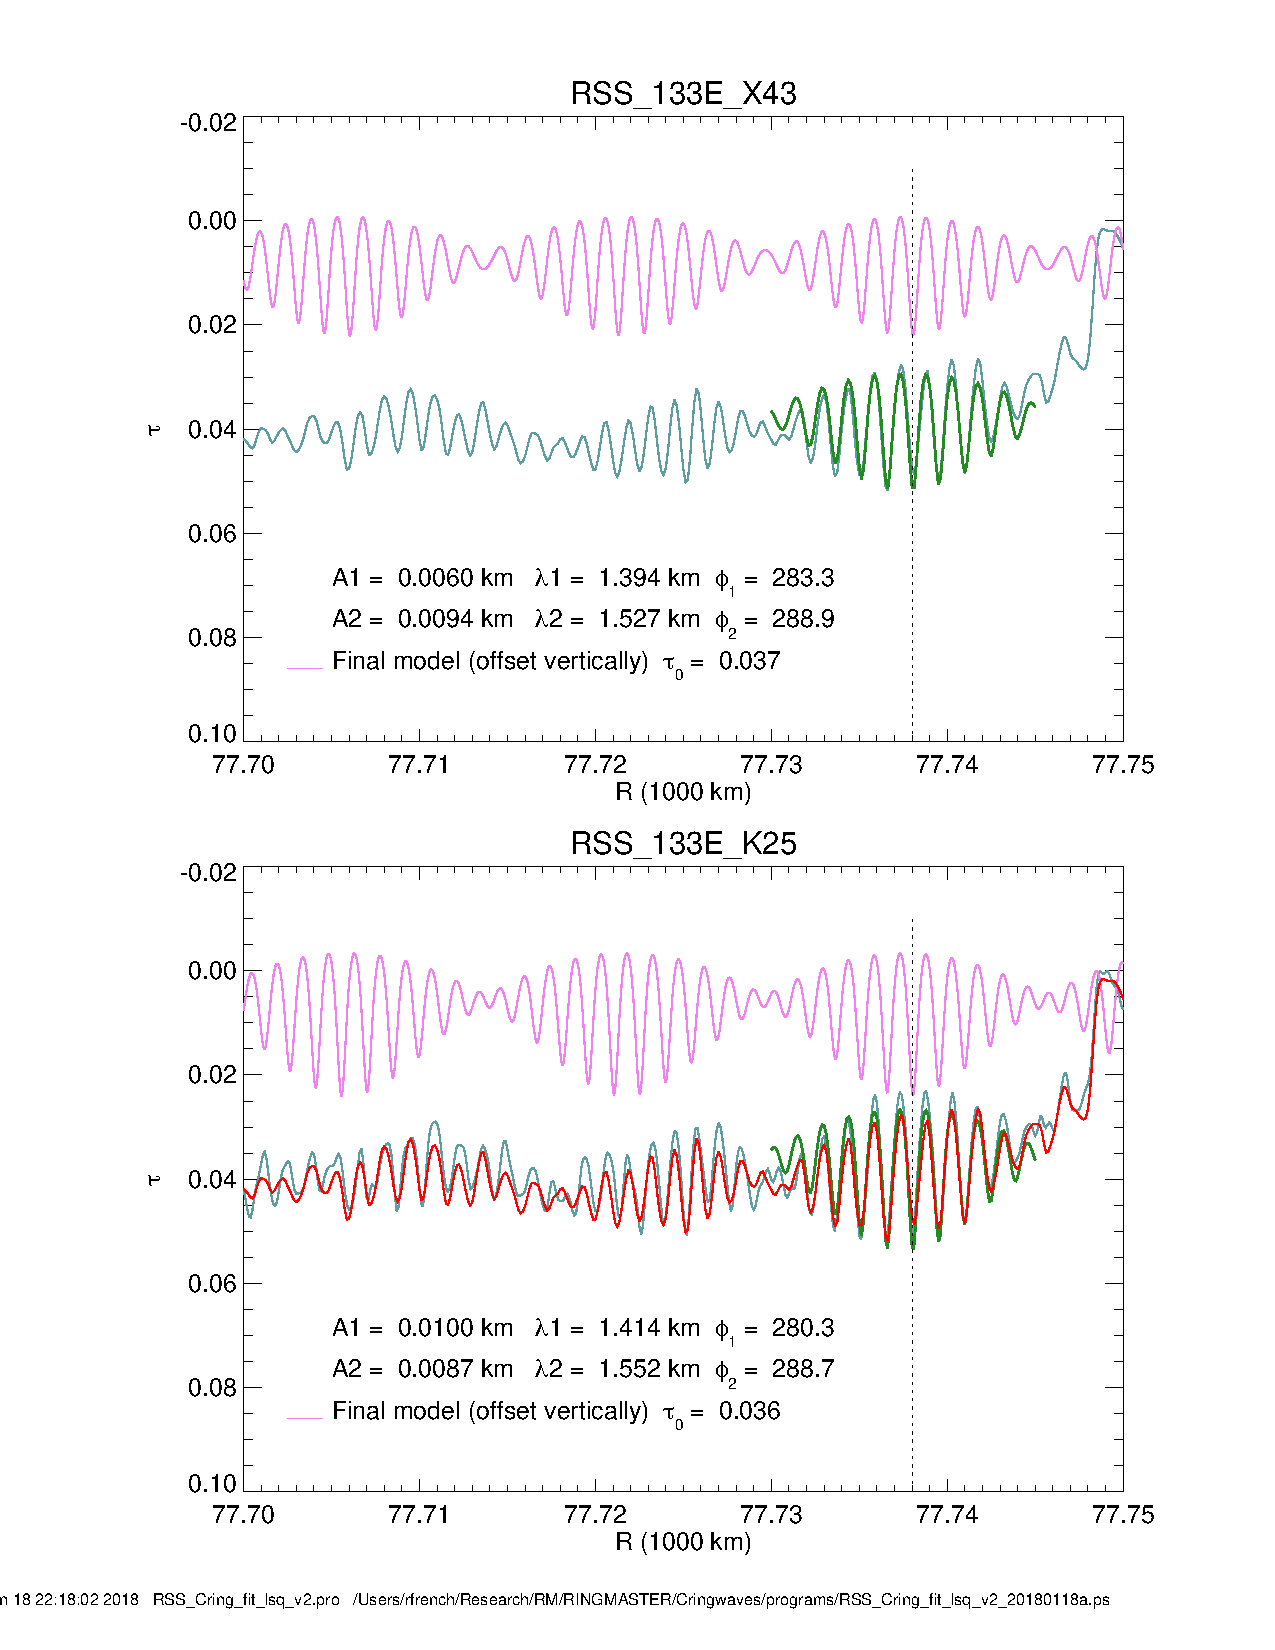
\includegraphics[width=\textwidth]{RSS_Cring_fit_lsq_v2_20180118a}
\end{figure}
\subsubsection{\footnotesize RE: Something Fishy in C-Ring Ripples}
Hi, all - I just plotted tau vs r for 
\begin{lstlisting}[language=bash]
2018_1_18_gjs_rev133_E_K25_77700_77500_350m_res.sav 
2018_1_18_gjs_rev133_E_X43_77700_77750_350_res.sav
\end{lstlisting}
See the attached fig. Qualitatively, they look pretty similar, but the X and Ka ripples quickly get out of phase, which makes me suspicious that something is wrong with the reconstruction or with the radius scale used for the two inversions. Our physical interpretation of the ripples is that they are due to corrugations in the surface of the rings, which should appear nearly similar at X and Ka bands (although we are looking at them from different earthbased stations, which makes things slightly different - do we have any ripple observations at X and Ka band from the SAME DSN complex? Glenn, when you compared Essam's X and Ka band retrievals, did you find this big a difference? (Red is X band; white is Ka band). One good test would be to overplot retrievals of the same data at different resolutions to confirm that the radii agree. Some further thoughts:
\begin{enumerate}
    \item Could one of you plot larger extents of the data to find sharp-edged rings, and see if they line up in radius for these two data sets? That would be a good test of the radius scale
    \item Can you look to see if there are ANY C ring ripple observations made from the same DSN complex but at different wavelengths? It's possible that the differences are due to the slightly different viewing geometry of the waves from the two observatories, but to explore that quantitatively, we need to know the difference the azimuth angle between the two data sets - can one of you track that down?
\end{enumerate}
If we can show:
\begin{enumerate}
    \item That the data sets have good radius scales by showing that the other rings line up fine
    \item That, when viewed from the same DSN, different wavelengths show the same features then there is a fun geometry problem that we can do to try to predict what a rippled ring should look like when viewed from slightly different angles - what we are interpreting as a difference in radius may have a different explanation that would be fun to try to model.
\end{enumerate}
If the data sets DON'T match up in radius, then we need to understand that, since it could be a sign that our reconstructions have a problem, so this is a high priority thing to explore. For completeness, I think we should run the inversions for all of the C ring ripples this spring, once we get our pipeline working efficiently! -Dick
\begin{figure}[H]
    \centering
    \includegraphics[width=\textwidth]{CringX43-red-vs-K25Rev133_350m_res}
\end{figure}
\subsubsection{\footnotesize RE: Time Test and Questions}
I ran S-Band at 250m resolution to see what would happen, and I found something interesting.
One would expect the time to compute a point would decrease with window size, and to some extent that happens. But for rev-125, w(r) does decrease yet the computation time per point varied almost sinusoidally. The entire computation took 22 hours, and had computation times per point ranging from 1 point per 5 seconds to 1000 points per second, again this varying happening periodically. I'm wondering if this is a memory thing. -Ryan\\
One point per five seconds probably means that some disk swapping is happening, which would be an indication of a memory issue. Two things to do:
\begin{enumerate}
    \item In IDL, type help,/mem and let me know what it says for this rev-125 job
    \item In a separate maxwell terminal window, type: ps au
\end{enumerate}
\subsubsection{\footnotesize RE: Top Priorities}
Hi, Ryan - By this weekend we need the final version of the Huygens and Titan ringlet plots from Rev007E for the Interim Report, and your first stab at a paragraph or two about what our GitHub documentation and submission plan will be. Could you put those two tasks at the top of your list? As I mentioned before, I can tweak the details of the figures to resemble Essam's, so don't spend lots of time on the format of the figs - I'm more concerned about knowing how well our curves reproduce his and having the appropriate savefiles to make the final plots. -Dick
\subsubsection{\footnotesize RE: Updates 01/23/2018}
v4.1 is done, it's v4 but with little bugs removed. I found out max(a,b) does nothing, and it needs to be max([a,b]), so that's been fixed everywhere. In the inversion page, about 10 variables that are a few thousand points long are defined inside the for loop everytime, this is a leftover of v1/v2 that was never corrected for. A time comparison of v4 vs v4.1 on rev007 E is 78 seconds to 76 seconds. I'm wondering if it'll be a bigger difference for revs that need larger windows, as this loading into memory is no longer included. A v5 is also done now. It uses an integral, rather than the convolution theorem/FFTs, and also includes the corrections from v4.1. Interestingly enough, it ran the fastest at 71 seconds. Note: Neither v4 nor v4.1 use powers of 2 in the FFT. This may be why v5 is fastest (3 FFT's versus 1 Total command). Below is the Encke Gap, Maxwell Ringlet, and v4-v5 of the Maxwell gap. v4 is white, v5 is red. For some reason, that completely eludes me right now, v4 is lagging behind v5 by a single point. I've made save files for rev007\_E for the interim report, but there was some error in the normalization so I don't think these should be used. I believe Jolene is making a new save file to be run. -Ryan
\begin{figure}[H]
    \centering
    \begin{subfigure}[b]{0.32\textwidth}
        \includegraphics[width=\textwidth]{Encke_Gap}
    \end{subfigure}
    \begin{subfigure}[b]{0.32\textwidth}
        \includegraphics[width=\textwidth]{Maxwell}
    \end{subfigure}
    \begin{subfigure}[b]{0.32\textwidth}
        \includegraphics[width=\textwidth]{Maxwell_v4-v5}
    \end{subfigure}
\end{figure}
Thanks for this promising update. Could you plot the difference between v4.1 and v5 after you shift by one bin? I'd like to see how big the difference is at that point. I'm sure it will be possible to track down the off-by-one error at some point. 
All of this suggests that the FFT part of the code is very fast compared to the computation of Psi, which probably accounts for the TOTAL version being comparably fast or even faster - in a way, that's really good news, since it means that we can simplify the production code by using the Matched Filter everywhere. PS Jolene is going back to the old Rev7 inversions for the interim report, since that is what gave the best agreement with Essam before changes to the normalization. You should check with her to see what versions she's using. The Titan ringlet is a special case, since Essam is using 100 m and 1 km  and 10 km inversions - whatever you have in hand that gives the best match to his is what we should use for the report, but we need to include in our ISSUES AND CONCERNS notes on our team meeting notes pages that we'll need to resolve all of this eventually. Glenn is working on a Python spline routine, and I think we should defer until we are in the Python coding stage our final choices of normalizations. -Dick
Below is v4.1 vs v5 with a 250 meter shift. They are practically identical. Below that is the difference of v4.1 and v5 with a 250m shift (1 bin). -Ryan
\begin{figure}[H]
    \centering
    \begin{subfigure}[b]{0.49\textwidth}
        \includegraphics[width=\textwidth]{Maxwell_1_Bin_Shift}
    \end{subfigure}
        \begin{subfigure}[b]{0.49\textwidth}
        \includegraphics[width=\textwidth]{Maxwell_250m}
    \end{subfigure}
\end{figure}
Thanks, Ryan - They do indeed look very similar! Once the off by a bin origin gets identified, I think we might want to continue to use the straightforward integration version - do you agree? It will be easiest to document, and we won't need users to install FFTW. By the way, what is the window width compared to the width of the ring? What do you make of the inverse symmetry about the midpoint of the lower plot - if you invert the RHS and fold it about the middle, the two curves look almost identical. I'd like to understand the origin of that pattern, if possible, even though it is below the level of practical significance. Could it be related to a slightly different way in which the window is centered in the two calculations? If you use Essam's savefile for Rev007E and his normalized diffraction pattern, how well do your two methods (V4.1 and V5) compare to his diffraction-corrected profile? Could you plot up that difference? I'd like to include that in our interim report in some fashion. -Dick\\
My guess is that the shift is not quite 1 bin, but 1.1 bin or something like that. That up-spike down-spike seems reminiscent of the offset we had back in November. -Ryan\\
One possible way to resolve this would be to do a forward and inverse problem for a translucent ring of a given optical depth and to compare the V4.1 and V5 results with the expected results from an analytic solution. That's how I usually try to track down finicky offsets like this - to try to reproduce a result with an analytic solution. (The one you did using Fresel integrals.) -Dick\\
v4.1 is doing the shifting, not v5. I compared the two with Essams files:
\begin{lstlisting}[language=bash]
../../../../data/RSSringoccs/savefiles/RSS_007E_X43_23MAR09.sav
\end{lstlisting}
-Ryan
Ok, that's good to know. Does that mean that V4.0 was shifting as well? Could you send me plots of the V5 comparison with Essam's result? -Dick\\
Final update for the night: I ran res\_char with v5, and using the optimal resolution gave a max error of 0.3\%. If you recall, v3 had a 2\% maximum error (The L\_infinity norm). The error is now on the same order of magnitude as the v4.1 vs v5 max error, which is also promising. The optimization code ran at 50m intervals, I'll use a finer interval to try and home in on sqrt(2), see where the best one is. I'll Have finalized plots ready for tomorrow morning, and you can do the IDL plotting magic. Just got your message, I'll make the plot comparison for v4.1 and v5 now. v4 used and even number of points per window, and v4.1 uses an odd number of points, so I believe this shifts the bin over, explaining the discrepancy between v4 and v4.1. v4.1 and v5 both use odd, so I don't know where the shift comes from there. Here you are. The first one is v5, and the second v4.1. Once v4.1 is shifted, the max error is 0.38\%, still better than before. -Ryan
\begin{figure}[H]
    \centering
    \begin{subfigure}[b]{0.49\textwidth}
        \includegraphics[width=\textwidth]{Maxwell_Our_Geo_Essam_Data}
    \end{subfigure}
    \begin{subfigure}[b]{0.49\textwidth}
        \includegraphics[width=\textwidth]{images/Maxwell_v4_1.png}
    \end{subfigure}
\end{figure}
Great - I'll be interested to find out what scale factor you applied to W. By the way, I think we discussed the possibility that this scale factor might be variable across the rings -- or not. Either one would help us diagnose the difference between Essam's approach and ours in defining $\Delta R_{\rm eff}$ -Dick
\subsubsection{\footnotesize RE: Comparison of Rev007 E Save Files}
I've made comparisons of all 4 save files, using the v4.1 reconstruction code, and have overplotted Essam's results as well.
\begin{figure}[H]
    \centering
    \begin{subfigure}[b]{0.49\textwidth}
        \includegraphics[width=\textwidth]{Maxwell_v4_1_Code_v0_Save_File}
        \caption{v0 Oct 30 08:24 rev007\_E\_X.sav}
    \end{subfigure}
    \begin{subfigure}[b]{0.49\textwidth}
        \includegraphics[width=\textwidth,trim={0.4in 0 0.4in 0},clip]{Maxwell_v4_1_Code_v1_Save_File}
        \caption{v1 Jan 3 13:02 Rev007\_E\_X43\_struct\_input.sav}
    \end{subfigure}
    \begin{subfigure}[b]{0.49\textwidth}
        \includegraphics[width=\textwidth]{Maxwell_v4_1_Code_v2_Save_File}
        \caption{v2 Jan 11 23:33 Rev007\_E\_X43\_struct\_input\_v2.sav}
    \end{subfigure}
    \begin{subfigure}[b]{0.49\textwidth}
        \includegraphics[width=\textwidth,trim={0.3in 0 0.3in 0},clip]{Maxwell_v4_1_Code_v3_Save_File}
        \caption{v3 Jan 21 23:44 Rev007\_E\_X43\_struct\_input\_v3.sav}
    \end{subfigure}
\end{figure}
Directory containing those files:
\begin{lstlisting}[language=bash,basicstyle=\footnotesize]
/Volumes/rmaguire001/Research/TC2017/rmaguire/v4/v4_1/outfiles
2018_01_24_rev007_E_X43_samp_250_range_70000_145000_res_1000m_input_v2.sav
2018_01_24_rev007_E_X43_samp_250_range_70000_145000_res_1000m_input_v3.sav
2018_01_24_rev007_E_X43_samp_250_range_70000_145000_res_1000m_input_v1.sav
2018_01_24_rev007_E_X43_samp_250_range_70000_145000_res_1000m_input_v0.sav
\end{lstlisting}
\begin{figure}[H]
    \centering
    \begin{subfigure}[b]{0.49\textwidth}
        \includegraphics[width=\textwidth]{Maxwell_v4_1_vs_Essam}
    \end{subfigure}
    \begin{subfigure}[b]{0.49\textwidth}
        \includegraphics[width=\textwidth,trim={0.3in 0 0.3in 0},clip]{Maxwell_v4_1_Minus_Essam}
    \end{subfigure}
\end{figure}
To make this I modified and commented out some parts of the following code:\\
/Volumes/rmaguire001/Research/TC2017/rmaguire/v4/v4\_1/resolution\_characterization/rjm\_func\_inverse\_resolution.pro\\
I've made a dedicated code to reproduce this plot:\\
/Volumes/rmaguire001/Research/TC2017/rmaguire/v5/compare/rjm\_diff\_corr\_compare.pro
\subsubsection{\footnotesize RE: Titan Ringlet Plots}
Hi, Ryan - When you have a chance would you send me a plot (and location of plotting program) that does your best reproduce Essam's Titan ringlet plots for Rev007E from the User's Guide (100m, 1 km, and 10 km resolution)? 
Also, could you process the F ring profiles Glenn did (rev 123 or rev 125, S, X, Ka) at 100-m resolution? He may need to supply you with 50-m resolution files. -Dick\\
There is a code that uses v5 to make plots and compare with Essam, using Essam's data:\\
/Volumes/dione\_raid2/Research/TC2017/rmaguire/v5/compare/rjm\_diff\_corr\_compare.pro
The inputs are at the top of the code:
\begin{itemize}
    \item WType - Only 'kb25' or 'kbmod' are allowed for simplicity.
    \item range = [start,end]
    \item res\_km - a double for resolution, in kilometers.
\end{itemize}
At the bottom of the code is the filename you wish to save the output as:\\
save, r, tau\_tc, power\_tc, power\_vals\_EAM, tau\_norm\_vals\_EAM,\$\\
filename = 'comparisons/2018\_01\_24\_rev007\_E\_X43\_Essam\_Comparison\_Maxwell\_Ringlet\_res\_1000m\_v5\_code\_2.sav'
\begin{figure}[H]
    \centering
    \begin{subfigure}[b]{0.49\textwidth}
        \includegraphics[width=\textwidth]{Maxwell_v5}
    \end{subfigure}
    \begin{subfigure}[b]{0.49\textwidth}
        \includegraphics[width=\textwidth]{Titan_v5}
    \end{subfigure}
\end{figure}
tau\_tc, power\_tc, power\_vals\_EAM, tau\_norm\_vals\_EAM are now saved at:\\
/TC2017/rmaguire/v5/compare/comparisons/2018\_01\_25\_rev007\_E\_X43\_Essam\_Comparison\_Maxwell\_Ringlet\_res\_1000m\_v5\_code\_2.sav\\
/TC2017/rmaguire/v5/compare/comparisons/2018\_01\_25\_rev007\_E\_X43\_Essam\_Comparison\_Titan\_Ringlet\_res\_1000m\_v5\_code\_1.sav\\
Jolene made modifications so that our v2 savefile is used with v5 reconstruction, and then compares with Essam:\\
/Volumes/dione\_raid2/Research/TC2017/rmaguire/v5/compare/rjm\_diff\_corr\_compare.pro\\
I haven't looked over the code, but she showed me the plots for the Maxwell ringlet and they looked very good. Yesterday I discovered that, due to large window sizes, the Riemann sum that is used in v5 cannot adequately capture the nature of the rapid oscillations that exp(ipsi) has. So rev-133 and rev-123 should use v4.1. For rev007, even at 100m resolution, the windows are small enough that the Riemann sum captures the same amount of detail as the FFT. I'm actually curious to find out what form of integration FFT uses. Last night I tried Simpson and Newton-Cotes integration, rather than just TOTAL, but both seemed rather poor for rev133. Also note, a quadratic fit to psi for the c-ring ripples is horrible. Indeed, a quartic fit was pretty bad ass well. A 6th degree polynomial fit incredibly well, however. The fact that psi can still be fit very well by a polynomial demonstrates why FFT works so well. I will make a v4.1 version of this compare program now. Should be done soon.
\subsubsection{\footnotesize RE: Updates 01/26/2018}
I'm going to make an updated version of that compare program and add the figures to the interim report now (I think I've got the hang of the plotting routine). If you don't like the figures I add, just let me know. Here's the google doc that I've updated. Let me know if there's anything more pressing to do today. (I intend to do the paragraph about Github once the figures are up). I'm also going to do a run through of the entire .tex file and get rid of the errors (We have 7).
\begin{figure}[H]
    \centering
    \begin{subfigure}[b]{0.49\textwidth}
        \includegraphics[width=\textwidth]{F-Ring}
    \end{subfigure}
    \begin{subfigure}[b]{0.49\textwidth}
        \includegraphics[width=\textwidth]{F-Ring_Zoomed_In}
    \end{subfigure}
\end{figure}
Ryan - Blue means done. Red means description.
\begin{itemize}
    \item \textcolor{blue}{Create your version of Figs 6 and 8 to be included in the interim report (send primitive version of plot program to Dick, who can reformat this to mimic Essam’s style and add it to the interim report) - rjm\_diff\_corr\_compare.pro}
    \item \textcolor{blue}{Include phase in the out\_struct, change the v4 code to do this.}
    \item \textcolor{blue}{Use standard range for reconstruction: RANGE = [70000,145000]}
    \item \textcolor{blue}{Add a listings example: Using the lstlisting environment} - \textcolor{red}{IDL Examples page in TC doc.}
    \item \textcolor{blue}{Contact Glenn and Jolene about the appropriate input files for you to use for the final Rev007 1 km reconstructions for Jolene to post in our prototype PDS directories, crank out those reconstructions using the best assumed resolution to match Essam's.} - \textcolor{red}{Use Rev007\_E\_X43\_struct\_input\_v2.sav for rev 7.}
    \begin{itemize}
        \item \textcolor{red}{Compare rev007 E phase with Essams - rmaguire/v5/compare/rjm\_diff\_corr\_compare.pro uses Essam’s data, and compares the TC reconstruction to Essam’s reconstruction. V5 has 0.3\% error in power. Phase matches up very well.}
    \end{itemize}
    \item \textcolor{blue}{Do the same for the Rev 133, and send files to Glenn so that he can produce diffraction-corrected profiles for Fig. 12 of the interim report.}
    \begin{itemize}
        \item \textcolor{blue}{Make reconstruction fro rev-123 S, X, Ka for F-ring. Replace Dick’s figures in interim report. - Half done. Have not added figures to report.}
        \item \textcolor{blue}{Use Essam’s data for rev-133 and compare reconstructions.}
        \begin{itemize}
            \item \textcolor{red}{Error in doing so for rev-133 with v5. The Riemann sum method for the massive windows that rev-133 has is insufficient in capturing the details of the rapidly oscillating exp(ipsi). Use v4.1 or v4 for rev-133 and rev-123.}
        \end{itemize}
    \end{itemize}
    \item Show professor french how to make folders and subfolders in sharelatex.
    \item \textcolor{blue}{I don't think Essam detected the F ring on Rev 133, but take a look anyway at your reconstruction in the expected vicinity of the F ring ($\pm$ about 300 km of 140219 km)}
    \begin{itemize}
        \item \textcolor{blue}{F-Ring is 1km in width, roughly. Use appropriate resolutions. - S-Band at 500m resolution detected it.}
    \end{itemize}
    \item \textcolor{blue}{Try your idea of improving your 10 km resolution model for the Titan ringlet, to compare with the User's Guide version. Use 250m resolution for this.} - \textcolor{red}{If I cheat and multiply by about 5, and smooth a wee bit, it looks great…}
    \item Write a paragraph or two for the Interim Report about the envisioned structure of our software contribution to GitHub, and the two levels of documentation we'll provide -- a "just enough information" to get started, with examples, and a much more detailed version that will take us from start to finish.
    \item \textcolor{blue}{Have you succeeded in doing a direct integration, without FFTs, for the inversion process? This would be good to have working, and to know the time it takes.} - \textcolor{red}{v5 is done. For rev007 E it matches better to Essam’s reconstruction than v4.1, and also is computed in a shorter amount of time. For rev-133 the integral is insufficient. Need to look into better numerical integration techniques.}
    \item Update your time test of how long an inversion takes using FFTs that are $2^n$ vs random length FFTs, and document the results.
    \item You'd worked on a 'forward' code that would produce a synthetic diffraction pattern for a given occultation geometry and assumed radial profile of normal optical depth. This would be a great addition to our software package and would provide a nice test of our inversion code, to be able to retrieve the input optical depth profile by inverting the synthetic diffraction pattern.
    \item Start thinking about the organization of our pipeline processing - a flow chart, if not actual program and procedure names - and especially about how and where users could enter the process mid-stream to perform diffraction corrections to snippets of data at requested resolutions without having to go through the entire preprocessing procedure for an entire RSR file. - Ryan will use LaTex to format what we wrote on the board
    \item I'd like to get our outlined pipeline process agreed on before we start translating code into Python in earnest, but if you want to do some early investigation into getting FFTW working in Python, that would be helpful.
-Ryan\\
Sounds good, Ryan - I took a look at V5 code today and I'd like to understand why v5 fails and FFT succeeds for wide windows - why does the FFT succeed and sum fail? If we have insufficient info in exp(ispi) for sum, why doesn't this bite us in the FFT? That sounds like an undersampling problem that should affect both methods. I wonder if it is a precision problem instead, which we can explore by looking at the code together. See you later this afternoon! -Dick\\
I did some checking and it is indeed a window thing, and not a geometry thing. For rev-133, at 10km resolution, v4.1 and v5 match almost exactly. My hunch for the inefficiency of the midpoint rule comes from the fact that I got a better match using simpson's rule than using total (See rjm\_func\_simpson). It's still a poor match, but the L\_inf norm is a bit smaller. I have an idea to test if the fault lies with summing that I can try in mathematica. If it is not the TOTAL commands fault, there's a very interesting question: Which one is correct? After all, the point of FFT is to mimic TOTAL, not the other way around... -Ryan
\end{itemize}
\subsubsection{\footnotesize RE: Good Plots}
IDL\_pipeline\_v2/gjs\_progress\_report/rjm\_fig\_3-12/gjs\_rev7E\_X43\_huygens\_1km.pro\\
For legends, you can make actual legends using the plot function. However, the plot function’s pretty janky so nobody uses it. In the plot procedure (which all the cool cats use), you can just add text to the plot using “xyouts”. For making arrows, there’s an arrow procedure in IDL where you can just specify the start and end points of the arrow. I have a weird problem where I don’t actually have a procedure named arrow, but instead I have one named “arrow\_internal”. If you end up having the same problem where you only have this “arrow\_internal” thing, then you can still use all the same syntax and everything that’s online for the arrow procedure - you just have to say “arrow\_internal” for every time they say “arrow”.
\subsubsection{\footnotesize RE: Post-Diffraction Correction Residual Phase}
Hi, all, esp. Ryan - I'm puzzled by the post-diffraction correction residual phase for the Titan ringlet in the plot now in the interim report. For the Huygens ringlet, the phase matches Essam's quite well, but for the Titan ringlet the 1 km results are quite poor, with far more structure and larger amplitude than Essam's. A clue about what is going on might be the asymmetry of the scatter in the phase, which is mostly positive and only slightly negative, which I would not expect. On the other hand, the POWER calculation looks good - tau agrees with Essam's. So, that means that $I^{2}+Q^{2}$ is OK but $atan(Q,I)$ is not. Ryan, would you first confirm that v4.1 and v5 give the same results for residual phase, and double-check your calculation of residual phase for Titan compared to Huygens ringlets? Did you use exactly the same code and input files for the two cases? I think there must be some difference, other than the Titan ringlet being more opaque than the Huygens ringlet. -Dick
I found the error. v5 and v4.1 produce near identical phases. The problem is that the 50m file was used, for the sake of being able to produce the 100m plots. If the v2 250m spacing file is used, you get a very good match. -Ryan
\subsubsection{\footnotesize RE: An Interesting Revelation}
While there is no mention of this in any of the papers, I tried 'normalizing' the reconstructed power by the following factor:
\begin{equation*}
    \frac{\int_{-\infty}^{\infty}w(\rho-\rho_{0})e^{i\psi}d\rho}{\int_{-\frac{W}{2}}^{\frac{W}{2}}e^{i\psi}d\rho}
\end{equation*}
This is the factor one would expect for free space. Anyways, if you look in:\\
/Volumes/dione\_raid2/Research/TC2017/rmaguire/v5/compare/comparisons/2018\_02\_02\_rjm\_diff\_corr\_compare\_rev007\_E\_X43\_Maxwell\_1km.ps\\
You'll notice that the difference in my reconstruction vs. Essam's has about a 0.001 offset in the free space range. The integral above is about 0.99 for the Maxwell range. This has me thinking a similar normalization factor must be used for 10km. I was wondering if I should include this in the report. Any thoughts? -Ryan
I've wondered about this, too, Ryan - why don't you try this for the 10km case and see what happens? Regarding the offset of 0.001 in the free space range, is this a difference you get when you use Essam's diffraction pattern? That's the comparison we would want to perform - perhaps we can do some other test cases to see if there are systematic differences in reconstructed free-space power at other locations in the rings. For now, let's list normalization by the window as an open question, and get the main other pieces of the interim report written up -- could you take a stab at a few paragraphs about GitHub plans? That section was empty, last time I looked. Let's go over all of this later today. -Dick
\subsubsection{\footnotesize RE: A Though on Phase}
While looking through the v5 code, I noticed something. A while back I made psi positive, just because it matched Marouf, and then filed this under ‘Deal with later.’ Psi has nothing to do with phase, it is a purely geometrical factor. The correct integral is:
\begin{equation*}
    \int|\hat{T}|w(\rho-\rho_{0})e^{i(\theta-\psi)}d\rho
\end{equation*}
What is written is:
\begin{equation*}
    \int|\hat{T}|w(\rho-\rho_{0})e^{i(\theta+\psi)}d\rho
\end{equation*}
Now, if the phase is negative, this ‘almost’ swaps things back to normal (But it doesn’t exactly, which is really weird as to why it worked to begin with. This is actually quite amazing). But what if, rather than the phase being negative, T runs clockwise. That is $\hat{T}=|\hat{T}|e^{-i\theta}$. This would fix the integral equation, and would also explain why, in order to get reconstructed phase to match essam, we need to do $\arctan(\frac{\Re(T)}{\Im(T)}$. Essam never specifies a clockwise or counter-clockwise preference. A way to test this is with a forward code. If the forward diffraction of the reconstructed T has real and imaginary parts swapped, then we'll know his phase runs clockwise. I ran reconstruction with this new mathematical scheme, and got 0.05\% error on Maxwell, using Essam's data. I think I should keep this scheme, perhaps as a v5.1 or something like that, just in case we need to go back to the old one. Comparison can be found here:\\
rmaguire/v5/compare/comparisons/2018\_01\_25\_rev007\_E\_X43\_Essam\_Comparison\_Titan\_Ringlet\_res\_1000m\_v5\_code\_1.sav\\
-Ryan\\
I agree that changing the sign of theta is the same as assuming that the phase in the complex plane rotates clockwise rather than CCW. Eq 15 in the User's Guide looks to me like it is a CCW rotation, though. But is it that case that you get something different from a 0.05\% error on Maxwell when you change the sign and use the opposite sense of rotation? -Dick\\
The two different codes are: v5 $\hat{T}=|\hat{T}|e^{i\theta}$, $ker=we^{i\psi}$, v5.1 $\hat{T}=|\hat{T}|e^{-i\theta}$, $ker=we^{-i\psi}$. They both produce about 0.05\% errors. Also, I don't think a simply rotation would fix the phase. A rotation of pi/2 would give phase = atan(real / -imaginary). A rotation, and then a reflection, would give phase = atan(real/imaginary), which is what we're seeing, and which is what the clockwise phase would do. As to why the code that has a positive i psi in the exponential works, I have no idea. -Ryan
\subsubsection{\footnotesize RE: Cassini Radio Ring Occultations During the Finale}
I have not done this, but I think you would be safe if you simply left out the data some 100s of km outside of the rings. There are diffraction affects that modify the phase of the signal at high spatial frequencies that you presumably average over. If you have a specific orbital pass you'd like me to look into in more detail. I'd also check with Luciano and Paolo to see what they do about ring occultation data. -Dick\\
Dick, We are struggling mightily to get a gravity field for Saturn to use in the final reconstruction. It appears that the rings are affecting the radio signal during the 5 gravity passes and are corrupting the gravity fit. We find that deleting the data during the ring occultations really helps the fit. However, we are basing our occultation deletes on the assumed ring radii and the associated ring occultation model. Do you know if there has been a determination of the actual times that the radio signal was significantly affected by the rings? -Bob\\
HI, All - Here is a request from a JPL colleague - would you take a look at the X band data for the rev with 23 June 2017 periapse? This is one of the ones with strange geometry, where the rings are occulted several times. It will be a good test of our software and we'll be able to tell Bob whether we see strange effects due to the rings. Add this to your list for when you want to do something different. A starting point would be for Jolene to identify the filename and to compute the occultation geometry over the course of the RSS file - plotting R(t) will look strange, I think! I'd still like to keep on schedule to get our interim report working. Ryan, let's start defining phase in a way that will match Essam's and the inversion code -- let Glenn know how to change his codes to do this. This will make our phase plots agree with Essam's without changing anything, and we'll just report that to get a match, we use the definition of phase that corresponds to a clockwise rotation in the complex plane - is that what you concluded, Ryan? -DF
\subsubsection{\footnotesize RE: Inaccuracy of v5}
\subsection{Some IDL Examples}
\subsubsection{Converting Between B1950 and J2000}
\begin{lstlisting}[language=bash,basicstyle=\footnotesize]
; Import NAIF Leap Second counter.
IDL> CSPICE_furnsh, 'naif0012.tls'
; Create Transformation matrix from B2950 to J2000
IDL> CSPICE_pxform, 'B1950', 'J2000', 0., matrix
IDL> matrix
    0.99992570795236291   -0.01117893813777013   -0.0048590038153592703
    0.01117893812642769    0.99993751334998870   -2.7162594714247041e-05
    0.00485900384145442   -2.7157926258510777e-05 0.99998819460237420
;Saturn's Pole in 1981 had RA=38.409 and DEC=83.324, in degrees, in the B1950 system.
;Create a unit vector pointing in the direction of Saturn's pole.
IDL> CSPICE_radrec, 1.d0, 38.409d0*CSPICE_rpd(), 83.324d0*CSPICE_rpd(), nhat 
; Get unit vector in the J2000 coordinates.
IDL> nhat2 = matrix##nhat                                                    
IDL> nhat2
     0.085456479386769341
     0.073212537409663367
      0.99364838574661674
; Make nhat2 into a vector.
IDL> nhat2 = reform(nhat2)
; Convert unit vector to RA and DEC in J2000.
IDL> CSPICE_recrad, nhat2, r, RA, DEC
; Check Results
IDL> print, r, RA, DEC
       1.0000000       40.587426       83.538850
\end{lstlisting}
\subsubsection{Using Icy to Retrieve State Vectors and Light Time Values for 1000 Ephemeris Times}
\begin{lstlisting}[language=bash,basicstyle=\footnotesize]
;Create array of 1000 ephemeris times with step size of 10 hours, starting July 1, 2005.
IDL> cspice_str2et, 'July 1, 2005', start
IDL> et = dindgen( 1000 )*36000.d + start
; Retrieve the state vectors and corresponding light times fro Mars to Earth at each et,
; in the J2000 frame, using LT+S aberration correction.
IDL> cspice_spkezr, 'Earth', et, 'J2000', 'LT+S', 'MARS', state, ltime
; ccess the ith state 6-vector corresponding to the ith et.
IDL> state_i = state[*,i]
; Convert the et vector from the previous example to UTC calendar strings.
IDL> format = 'C'
IDL> prec = 3
IDL> cspice_et2utc, et, format, prec, utcstr
; Access the ith string of utcstr.
IDL> utcstr_i = utcstr[i]
; Convert the position components of the N state vectors to latitudinal coordinates.
IDL> cspice_reclat, state[0:2,*], radius, latitude, longitude
; The call returns three double precision variables: radius, latitude, longitude.
\end{lstlisting}
\subsubsection{Calculate and Plot the Trajectory of Cassini in J2000}
\begin{lstlisting}[language=bash,basicstyle=\footnotesize] 
;Load the following kernels.
IDL> cspice_furnsh, 'naif0012.tls'
IDL> cspice_furnsh, 'de421.bsp'
IDL> cspice_furnsh, 'pck00010.tpc'
IDL> cspice_furnsh, '030201AP_SK_SM546_T45.bsp' 
;Define the number of divisions of the time interval and the time interval.
IDL> STEP = 10000
IDL> utc = [ 'Jun 20, 2004', 'Dec 1, 2005' ]
IDL> cspice_str2et, utc, et
IDL> times = dindgen(STEP)*(et[1]-et[0])/STEP + et[0]
IDL> cspice_spkpos, 'Cassini', times, 'J2000', 'NONE', 'SATURN BARYCENTER', pos, ltime
;Plot the resulting trajectory.
IDL> x = pos[0,*]
IDL> y = pos[1,*]
IDL> z = pos[2,*]
IDL> iplot, x, y, z
IDL> cspice_kclear
\end{lstlisting}
Here is the same code for MATLAB (Mice)
 \begin{lstlisting}[language=bash,basicstyle=\footnotesize]
% Define the number of divisions of the time interval.
STEP = 1000;
% Construct a meta kernel, "standard.tm?, which will be used to load the needed
% generic kernels: "naif0011.tls," "de421.bsp,? and "pck00010.tpc.?
% Load the generic kernels using the meta kernel, and a Cassini spk.
cspice_furnsh( { 'standard.tm', '/kernels/cassini/spk/030201AP_SK_SM546_T45.bsp'} )
et = cspice_str2et( {'Jun 20, 2004', 'Dec 1, 2005'} );
times = (0:STEP-1) * ( et(2) - et(1) )/STEP + et(1);
[pos,ltime]= cspice_spkpos( 'Cassini', times, 'J2000', 'NONE', 'SATURN BARYCENTER' );
% Plot the resulting trajectory.
x = pos(1,:);
y = pos(2,:);
z = pos(3,:);
plot3(x,y,z)
cspice_kclear
\end{lstlisting}
\section{Ryan's Progress Report}
\subsubsection{\footnotesize 07/17/2017}
\begin{enumerate}
    \item Found typos/errors in the geometry and equations pertaining to Occultations Observations of Titan's Atmosphere.
\end{enumerate}
\subsubsection{\scriptsize To Do's}
\begin{enumerate}
    \item Re-derive the equations involved in the geometry of an atmospheric occultation.
\end{enumerate}
\subsubsection{\footnotesize 07/19/2017}
\begin{enumerate}
    \item Derived the geometry of an Occultation Observation of Titan's Atmosphere. Found typos and some equations were incorrect.
    \item Worked with Jolene and Glenn and they showed me how to create Cassini's trajectory and find out where Cassini is.
    \item Continued reading through the User's Guide and taking detailed notes for later use.
\end{enumerate}
\subsubsection{\scriptsize To Do's}
\begin{enumerate}
    \item Finish reading the User's Guide and finish the notes.
\end{enumerate}
\subsubsection{\footnotesize 07/21/2017}
\begin{enumerate}
    \item Read through Marouf 1982 in great detail to better understand the geometry. Doubtful of certain claims.
    \item Read through Marouf 1986 to learn more about diffraction correction.
    \item Finished User's Guide. Wrote derivation of the geometry of Titan's atmospheric occultations, which we will not be working with.
\end{enumerate}
\subsubsection{\scriptsize To Do's}
\begin{enumerate}
    \item Learn about Fresnel Diffraction and go through old notes on Fourier Optics.
    \item If time permits, read Van de Huulst and Chandrasakhr. Both are crucial to the theory of occultations.
    \item Next week, start recreating figures from Marouf.
\end{enumerate}
\subsubsection{\footnotesize 07/24/2017}
\begin{enumerate}
    \item Found error in Marouf 1982. The paper claims Earth should lie in $xz-$plane, but it should not.
    \item Learned more about NAIF.
    \item Used Glenn's Ripcalc routine to find the ring radius for various points in time during the Voyager 1 flyby.
    \item Worked on understanding the geometry of Marouf 1986.
\end{enumerate}
\subsubsection*{\scriptsize To Do's}
\begin{enumerate}
    \item Learn the Mie Theory (Read Jackson and Whittet).
    \item Learn about the problem of scattering off a random ensemble of points. Read the App. Opt. articles.
    \item Recreate the figures and tables from Marouf 1982/1986. Justify various equations in both of these.
    \item Start on the diffraction reconstruction for Rev-7E.
\end{enumerate}
\subsubsection{\footnotesize 07/25/2017}
\begin{enumerate}
    \item Installed Python 3.5. Spiceypy works on Python, Canopy, and Jupyter.
    \item Archived all useful information from e-mails onto a write-up.
    \item Plotted Cassini's trajectory.
    \item Was able to use CSPICE on MATLAB.
    \item Found several parts of Marouf's Table 1 using the rip\_calc.pro routine.
\end{enumerate}
\subsubsection{\scriptsize{To Do's}}
\begin{enumerate}
    \item Finish recreating the remaining parts of Marouf 1986.
\end{enumerate}
\subsubsection{\footnotesize 07/27/2017}
\begin{enumerate}
    \item Went through more NAIF tutorials
    \item Began work on diffraction reconstruction
    \item Made most of table 1 from Marouf 1986
\end{enumerate}
\subsubsection{\footnotesize 07/28/2017}
\begin{enumerate}
    \item Continued working on Marouf 1986. Tried recreating figure 4.
\end{enumerate}
\subsubsection{\footnotesize 07/31/2017}
Time In:\ 5:07 A.M.\\
Time Out: 8:58 P.M. \hfill 15 Hours, 51 minutes\\
Coffee Break: 7:56 A.M. - 8:14 A.M. \hfill 18 Minutes\\
Lunch Break: 12:15 P.M. - 12:32 P.M. \hfill 17 Minutes\\
Dinner Break: 6:20 P.M. - 6:35 P.M. \hfill 15 Minutes\\
Total:\hfill 15 Hours, 1 minute
\begin{enumerate}
    \item Began typing up NAIF tutorials into RJM Cassini 2017 Latex Document. Kept essential and relevant information for use later on.
    \item Began working with SPK files, in particular trying to reproduce Marouf Table 1.
    \item Got stuck with some of the details of using the kernels. Will figure out tomorrow.
\end{enumerate}
\subsubsection{\footnotesize 08/02/2017}
Time In: 6:00 A.M.\\
Time Out: 7:38 P.M. \hfill 13 Hours, 38 minutes\\
Breakfast/Coffee: 6:02 - 6:20 \hfill 18 Minutes\\
Lunch Break: 1:20 P.M. - 1:30 P.M. \hfill 10 Minutes\\
Dinner Break: 6:19 P.M. - 6:28 P.M. \hfill 9 Minutes\\
Went to Boathouse: 1:48 P.M. - 2:20 P.M \hfill 32 Minutes\\
Total:\hfill 12 Hours, 29 Minutes
\begin{enumerate}
    \item Learned to use ripcalc.
    \item Learned how to implement the SPICE Toolkit for IDL computations.
    \item Made my own ripcalc routine.
    \item Compared my ripcalc routine against a variety of parameter changes (CN, LT, LT+S, and NONE aberration corrections).
    \item After some tweaking, my routine agrees with the Rev-7E results to within a few meters.
\end{enumerate}
\subsubsection{\footnotesize 08/04/2017
Time In: 5:35 A.M.\\
Time Out: 6:48 P.M.\hfill 13 Hours, 13 Minutes\\
Breakfast/Coffee: 6:00 A.M. - 6:17 A.M. \hfill 17 Minutes\\
Lunch Break: 12:09 P.M. - 12:17 P.M. \hfill 8 Minutes\\
Coffee Break: 3:58 P.M. - 4:11 P.M. \hfill 13 Minutes\\
Total: \hfill 12 Hours, 35 Minutes}
\begin{enumerate}
    \item Changed my ripcalc routine. My results for Voyager agree with professor French's rgf\_MTR86\_table1.pro to within a few centimeters.
    \item Began working on recreating figures $4$ and $5$.
    \item Updated my ripcalc to create all of table 1, similar to rgf\_MTR86\_table1.pro.
\end{enumerate}
\subsubsection{\footnotesize Week 07/31 - 08/04}
Total in Wellesley: \hfill 42 Hours, 42 Minutes\\
Total Worked: \hfill 40 Hours, 5 Minutes
\begin{enumerate}
    \item Successfully created Table 1 of Marouf. 
    \item Successfully derived the equation of $\psi$ in Marouf.
    \item Worked on reproducing figures $5$ and $4$. Expect to have this completed early next week.
    \item Began going over van de Huulst for the derivation of some basic equations in Marouf.
    \item Learned to use the NAIF Toolkit effectively and used in code.
\end{enumerate}
\subsubsection{\footnotesize 08/08/2017}
Time In: 5:12 A.M.\\
Time Out: 8:18 P.M. \hfill 15 Hours, 6 Minutes\\
Lunch Break: 11:52 A.M. - 12:14 P.M. \hfill 22 Minutes\\
Dinner Break: 5:30 P.M. - 6:01 P.M. \hfill 31 Minutes\\
Total: \hfill 14 Hours, 13 Minutes
\begin{enumerate}
    \item Reinstalled Mathematica (It wasn't working for some reason). It now works.
    \item Installed Microsoft Word from the Wellesley website.
    \item Worked on Figure 5. Was able to recreate $\Re\big[T(\rho)\big]$ in Mathematica using a hat function impulse profile.
    \item Successfully made figure $5$. 
    \item Made very rough plots of $T(\rho)$ for the above impulse profile using quadratic approximation.
\end{enumerate}
\subsubsection{\footnotesize 08/10/2017}
Time in: 5:53 A.M.\\
Time Out: 9:00 \hfill 15 Hours, 7 Minutes\\
Lunch Break: 12:12 P.M. - 12:26 P.M.\hfill 14 Minutes\\
Dinner Break: 6:00 P.M. - 6:10 P.M. \hfill 10 Minutes\\
Total: \hfill 14 Hours, 43 Minutes
\begin{enumerate}
    \item Read through Elliot (1984).
    \item Worked on diffraction correction code.
    \item Updated Cassini 2017 TeX document.
\end{enumerate}
\subsubsection{\footnotesize 08/11/2017}
\begin{enumerate}
    \item Worked on figure 4 of Marouf et al. 1986.
    \item Read Chylek's paper to understand the theory behind Fresnel diffraction.
    \item Learned about Hanning and Hamming windows.
    \item Learned about the limitations of various windows.
    \item Learned about Chebyshev and Kaiser-Bessel windows.
    \item Read Characteristics of Different Smoothing Windows
    \item Read through Understanding FFTs and Windowing
    \item Sucsessfully reproduced figure 4
\end{enumerate}
\subsubsection{\footnotesize Week 08/07 - 08/11}
Total in Wellesley: \hfill 30 Hours, 13 Minutes\\
Total Home: \hfill 12 Hours\\
Total Worked: \hfill 40 Hours, 56 Minutes
\begin{enumerate}
    \item Made Figure 5 from MTR86.
    \item Made figure 4 from MTR86.
    \item Made Table 3 from MTR86.
    \item Learned about windowing/taper functions.
    \item Began diffraction correction code.
    \item Read Chylek.
\end{enumerate}
\subsubsection{\footnotesize 08/14/2017}
Time In: 5:56 A.M.\\
Time Out: 7:28 P.M. \hfill 13 Hours, 32 Minutes\\
Lunch Break: 12:10 P.M. - 12:23 P.M. \hfill 13 Minutes\\
Dinner Break: 6:30 PM. - 6:40 P.M. \hfill 10 Minutes\\
Total: \hfill 13 Hours, 9 Minutes
\begin{enumerate}
    \item Added notes to the recreating of figure 4.
    \item Tried rsyncing, but it took over 5 hours.
    \item Made flow chart with Glenn and Jolene.
    \item Professor French directly rsynced. All set now.
    \item Worked with the Kaiser-Bessel window and learned about its properties. It does not tend to zero at the edges, but tends to $\frac{1}{I_{0}(\pi \alpha)}$
\end{enumerate}
\subsubsection{\footnotesize 08/16/2017}
Time In: 5:13 A.M.\\
Time Out: 6:44 P.M. \hfill 15 Hours, 31 Minutes\\
Lunch Break: 12:22 P.M. - 12:38 P.M. \hfill 16 Minutes\\
Dinner Break: 6:30 PM. - 6:45 P.M. \hfill 15 Minutes\\
Total: \hfill 13 Hours, 0 Minutes
\begin{enumerate}
    \item Went through and proved Shannon's Sampling Theorem.
    \item Studied the Fourier Transform and its uses.
    \item Read Introduction to Matched Filters.
\end{enumerate}
\subsubsection{\footnotesize 08/17/2017}
\begin{enumerate}
    \item Learned about the IDL routines used to perform diffraction correction.
    \item Looked more into the Kaiser-Bessel windows, and what happens as $\alpha$ varies.
\end{enumerate}
\subsubsection{\footnotesize 08/18/2017}
Time In: 5:18 A.M.\\
Time Out: 9:18 P.M. \hfill 16 Hours, 0 Minutes\\
Lunch Break: 12:00 P.M. - 12:30 P.M. \hfill 30 Minutes\\
Dinner Break: 6:00 P.M. - 6:30 P.M. \hfill 30 Minutes
\begin{enumerate}
    \item Got old hard drive working again. All of my data is back.
    \item Ran newest version of rjm\_diffraction\_correction.pro and it works.
    \item Tested various save files:
    \begin{enumerate}
        \item input\_rev7E\_avg\_iq\_16khz - Bad reconstruction. Crazy phase. The power reconstruction was squashed down to zero. This is an old file, however.
        \item input\_rev7E\_avg\_iq\_100m - Bad reconstruction. Jolene's save file that shifts the geometry by 100 meters in an attempt to fix offset. Offset comes from phase, not geometry. This is also an old file.
        \item input\_rev7E\_avg\_iq\_halfbin - Bad reconstruction. A different attempt to fix the offset. Old file.
        \item input\_rev7E\_avg\_iq\_predicts - Good reconstruction. Uses reconstructed frequency. Uses kernels from the trajectory of the spacecraft after the event. Still contains slope in the phase, which results in offset.
        \item input\_rev7E\_avg\_iq - Good reconstruction. Gets sky frequency from polynomials in RSR file. Runs same predicts program as reconstructed frequency.  Still contains slope in the phase, which results in offset.
        \item input\_rev123\_avg\_iq\_1khz - Crazy phase. Geometry is off by about 10 kilometers or so. Other than that, reconstruction is decent.
        input\_rev7E\_ourFFTpower\_16NperFFT\_more\_pts - Poor resolution. The slope is more gradual than Essam's. Phase is much better and the slope is removed (No more radial offset). 
        \item input\_rev7E\_schinder\_16NperFFT\_more\_pts - Similar to previous input. Wrong phi\_rad\_vals. 
        \item input\_rev7E\_schinder\_32NperFFT\_more\_pts - Same as before. Wrong phi\_rad\_vals.
        \item input\_rev7E\_schinder\_16NperFFT\_pad20\_more\_pts - Same as before. Wrong phi\_rad\_Vals.
    \end{enumerate}
    \item Changed the phi values from the save files Glenn gave me with the phi values from the save file Jolene gave me.
    \item Re-ran diffraction correction on the various save files with the correct phi values:
    \begin{enumerate}
        \item input\_rev7E\_ourFFTpower\_16NperFFT\_more\_pts - Very good match. The phase has been fixed.
        \item input\_rev7E\_schinder\_16NperFFT\_more\_pts - Nearly identical to the previous one. Good fit. Slope in phase mostly removed. Offset gone.
        \item input\_rev7E\_schinder\_16NperFFT\_pad20\_more\_pts - Good fit.
        \item input\_rev7E\_schinder\_32NperFFT\_more\_pts - Better fit than fit with padding.
    \end{enumerate}
\end{enumerate}
\subsubsection{\footnotesize 03/28/2018}
Time In: 5:03 A.M.\\
Time Out: 7:30 P.M.\hfill 14 Hours, 27 Minutes\\
Coffee Break: 5:58 A.M. - 6:10 A.M. \hfill 12 Minutes\\
Lunch Break: 1:28 P.M. - 2:12 P.M. \hfill 44 Minutes\\
Total: \hfill 13 Hours, 0 Minutes
\subsubsection{\scriptsize To Do}
Priorities
\begin{itemize}
    \item End to end pipeline in Python for Rev007 E, X43.
    \begin{itemize}
        \item *.cal
        \item *.geo
        \item *.obs
        \item *.tau
    \end{itemize}
    \item Learn how to make a GUI for the end-user.
    \begin{itemize}
        \item PyQt5
        \item TkInter
    \end{itemize}
    \item Learn about the $\alpha$ of a plot.
    \item Make interactive plot for rev007 E.
    \begin{itemize}
        \item Slides for plots to allow zooming in and out.
        \item Learn how to change plot scales.
        \item Explore layout options for GUI canvas.
    \end{itemize}
\end{itemize}
Think about user interactive parts.
\begin{itemize}
    \item Geometry
    \begin{itemize}
        \item Mindfully choose the RSR you want. Radial coverage, opening angle, etc.
    \end{itemize}
    \item Phase and power retreival
    \begin{itemize}
        \item Picking start and end SPM
        \item Choosing nots
        \item Choosing order of residual frequency fit
    \end{itemize}
    \item Diffraction reconstruction
    \begin{itemize}
        \item Choose resolution, window type, and range.
    \end{itemize}
\end{itemize}
\begin{table}[H]
    \centering
    \begin{tabular}{|c|c|c|c|}
        \hline
        To Do&J&G&R\\
        \hline
        Install Qt&\checkmark&\checkmark&\checkmark\\ 
        \hline
        Install PyQt5&\checkmark&\checkmark&\checkmark\\
        \hline
        Move example files&\checkmark&\checkmark&\checkmark\\
        \hline
    \end{tabular}
\end{table}
\subsubsection{\footnotesize 03/30/2018}
Time In: 6:59 A.M.\\
Time Out: 4:00 P.M.\hfill 9 Hours, 1 Minutes\\
Lunch Break: 1:32 P.M. - 2:13 P.M. \hfill 41 Minutes\\
Total: \hfill 8 Hours, 20 Minutes
\subsubsection{\scriptsize To Do:}
\begin{enumerate}
    \item Convert python code from reading a file to reading instances of classes.
    \item Fix python code to make the range a variable, not hard-lined into the code.
    \item Look at Essam's new directory structure.
    \item Look at Essam's diffraction profiles. Try to recreate his corrected profiles using the diffraction reconstruction code.
    \item Annotate code using team convention. Look at everyone else's code and compare and contrast styles.
\end{enumerate}
\normalsize
\clearpage
\section{Notes from the Team Meetings}
\subsection{2017/05/30}
\subsubsection{Goals}
\begin{enumerate}[nolistsep]
    \begin{multicols}{2}
        \item Overview of Cassini Mission.
        \item Overview of Team Goals.
        \item Team responsibilities.
        \item How we'll do our work.
        \item Familiarize with key resources.
        \item Procedures and skills needed.
        \item Analyze, preserve, and document\par
        RSS observations.
        \item Design data archive for PDS.
        \item Design open-source software for\par
        going from raw data to optical depth.
        \item Develop User's Guide.
    \end{multicols}
\end{enumerate}
Jolene:
\begin{enumerate}[nolistsep]
    \begin{multicols}{2}
        \item Download entire set of RSS raw data.
        \item Design format of data and software.
        \item Test Dick Simpson's MATLAB program.
        \item Reproduce "Browse" products for Rev007E.
        \item Design and produce "Browse" for each data set.
        \item Edit Revised RSS User's Guide.
    \end{multicols}
\end{enumerate}
Glenn:
\begin{enumerate}[nolistsep]
    \begin{multicols}{2}
        \item Convert data from raw to DLP.
        \item Develop expertise in DSP.
        \item Learn to use NAIF toolkit.
        \item Hey
        \item Sup
    \end{multicols}
\end{enumerate}
\subsubsection{Unacheived}
Hi!
\end{document}